\documentclass[12pt, a4paper]{article}
\usepackage[utf8]{inputenc}
\usepackage[T1]{fontenc}
\usepackage{geometry}
\geometry{top=1in, bottom=1in, left=1in, right=1in}
\usepackage{graphicx}
\usepackage{float}
\usepackage{xcolor}
\usepackage{amsmath, amssymb}
\usepackage{hyperref}
\usepackage{booktabs}
\usepackage{caption}
\usepackage{fancyhdr}
\usepackage{helvet}
\renewcommand{\familydefault}{\sfdefault} % Arial/Helvetica-like
\usepackage{setspace}
\setstretch{1.20} % Increased line spacing for readability and length

\pagestyle{fancy}
\fancyhf{}
\lhead{DSA5205 Project 2 --- Group 28}
\rhead{Multi-Strategy Asset Allocation on NVDA}
\cfoot{\thepage}

\hypersetup{
    colorlinks=true,
    linkcolor=blue,
    filecolor=magenta,      
    urlcolor=cyan,
    pdftitle={DSA5205 Project 2: Multi-Strategy Asset Allocation on NVDA},
}

\begin{document}

\begin{titlepage}
    \centering
    \vspace*{0.3in}
    {\LARGE\bfseries DSA5205 Machine Learning in Quantitative Finance\par}
    \vspace{0.3in}
    {\huge\bfseries Project 2: Design, Validate, and Analyze an Original Asset Trading Strategy\par}
    \vspace{0.2in}
    {\Large\itshape Systematic Multi-Strategy Quantitative Asset Allocation on NVIDIA (NVDA):\\
    Reconciling Mean Reversion, Macro Trend Following, and Volatility-Targeted Position Sizing\par}
    \vspace{0.4in}
    {\Large \textbf{Group 28}\par}
    \vspace{0.1in}
    {\large National University of Singapore\par}
    \vspace{0.1in}
    {\large Academic Year 2026/2027 \quad|\quad Submission Date: November 2026\par}
    \vspace{0.3in}

    \begin{table}[H]
    \centering
    \small
    \caption*{\textbf{Team Member Roster \& Contribution Matrix}}
    \begin{tabular}{p{3.2cm} p{3.0cm} p{8.5cm}}
    \toprule
    \textbf{Team Member} & \textbf{Core Module Ownership} & \textbf{Specific Technical \& Empirical Contributions} \\
    \midrule
    \textbf{Yu Jie} & Extension 1 Lead \newline Data Pipeline & Architected shared data ingestion (\texttt{src/data.py}), feature engineering (\texttt{src/features.py}), and Ridge Mean Reversion model with expanding TimeSeriesSplit CV (\texttt{src/model.py}, \texttt{src/backtest.py}). \\
    \midrule
    \textbf{Marco} & Extension 2 Lead \newline Momentum Research & Formulated 200-day Simple Moving Average regime filter and ML Momentum models (Ridge $L_2$ and Lasso $L_1$) to eliminate catastrophic drawdowns in the 2022 bear market (\texttt{scripts/run\_extension2\_momentum.py}). \\
    \midrule
    \textbf{Diana} & Extension 3 Lead \newline Showdown Harness & Developed dynamic volatility-targeted continuous position sizing (\texttt{src/strategy\_volatility.py}), automated unit test suite, and the unified 5-way showdown harness (\texttt{scripts/run\_consolidated\_showdown.py}). \\
    \midrule
    \textbf{All Members} & Academic Report \& Presentation & Equal collaboration across econometric narrative, latex synthesis, APA 7th referencing, code validation, and video presentation recordings (equal 1/3 speaking slots). \\
    \bottomrule
    \end{tabular}
    \end{table}

\end{titlepage}

\newpage
\tableofcontents
\newpage

\begin{abstract}
\textbf{Abstract} --- This quantitative asset pricing investigation designs, validates, and evaluates an institutional-grade, multi-strategy systematic trading framework on NVIDIA Corporation (\texttt{NVDA}) spanning the full 9-year cycle from January 2015 to January 2024. Addressing the fundamental market microstructure and macro regime dynamics of high-beta technology leaders, Group 28 formulates and pits three competing quantitative hypotheses against passive market benchmarks:
\begin{enumerate}
    \item \textbf{Extension 1 (Yu Jie --- Daily Mean Reversion):} An $L_2$-penalized Ridge regression model ($\alpha = 1000.0$) mapping historical return momentum and multi-scale moving average divergences to forward daily returns, exploiting transient liquidity dislocations (``buying the dip'').
    \item \textbf{Extension 2 (Marco --- Macro Trend \& Regularized Momentum):} A 200-day Simple Moving Average ($P_t > \text{SMA}_{200}$) regime-gating filter coupled with regularized machine learning momentum (Ridge and Lasso) designed to insulate capital from secular macroeconomic drawdowns.
    \item \textbf{Extension 3 (Diana --- Volatility-Targeted Position Sizing):} A continuous risk-managed allocation framework dynamically scaling daily exposure $w_t = \min\left(1.0, \frac{\sigma_{\text{target}}}{\max(\sigma_{t, 20\text{d}}, 10^{-6})}\right)$ with target volatility $\sigma_{\text{target}} = 40\%$ to mitigate volatility clustering and tail-risk drag.
\end{enumerate}
To enforce absolute academic and quantitative integrity, all strategies are executed with zero lookahead bias, forward-only StandardScaler scaling, and realistic Market-On-Close (MOC) execution deducting a uniform 10 basis points (0.10\%) transaction friction on turnover. 

In a unified out-of-sample showdown across 449 trading days (mid-2022 through 2023), Marco's 200-day SMA trend strategy achieves the highest risk-adjusted Sharpe ratio of \textbf{1.68} and curtails maximum drawdown to just \textbf{-19.30\%} by transitioning into 100\% cash throughout the 2022 bear market. Concurrently, Diana's volatility-targeted strategy resolves the classical ``volatility drag paradox'', delivering an annualized compound growth rate (CAGR) of \textbf{44.68\%} (outperforming unconstrained NVDA Buy \& Hold's 42.28\%) while slashing maximum drawdown from \textbf{-60.80\%} to \textbf{-42.45\%} ($\approx 18.35$ percentage points of capital preservation). Conversely, Yu Jie's dip-buying strategy documents the peril of the ``falling knife'' anomaly in bear regimes (CAGR: 32.31\%, MaxDD: -59.40\%, Sharpe: 0.85). We synthesize these empirical findings into a unified quantitative architecture that reconciles microstructure mean reversion with macro trend preservation.
\end{abstract}

\section{Introduction \& Economic Story}
\subsection{Theoretical Context in Quantitative Finance}
A central tenet of quantitative finance and empirical asset pricing is the identification and exploitation 
of market inefficiencies. In frictionless markets governed by the Efficient Market Hypothesis (Fama, 
1970), price changes follow a martingle difference sequence with respect to historical information sets, 
rendering past prices useless for forward capital allocation. Over subsequent decades, extensive empirical research uncovered persistent market anomalies categorized broadly into two competing market 
dynamics:
1. Time-Series Momentum: The tendency of assets with positive trailing performance over intermediate horizons (3 to 12 months) to continue outperforming (Jegadeesh \& Titman, 1993; Moskowitz 
et al., 2012).
2. Short-Term Mean Reversion:  The tendency of asset returns over short lookback horizons (1 to 
20 days) to reverse, reflecting behavioral overreactions, temporary liquidity shortages, and bid-ask 
bounce (Lehmann, 1990; Lo \& MacKinlay, 1990; Jegadeesh, 1990).
While momentum dominates macroeconomic and factor-based equity pricing, mean reversion operates 
as a fundamental market microstructure phenomenon. When unexpected negative news or localized 
liquidity demands strike an individual security, programmatic stop-losses, margin liquidations, and 
retail panic trigger exaggerated selling pressure that temporarily depresses market prices below their 
fundamental equilibria. Rational risk capital subsequently enters the market to absorb order imbalances, 
inducing a sharp corrective rebound.

\subsection{The ``Buy the Dip'' Hypothesis}
In popular financial parlance, this contrarian dynamic is colloquially termed ``Buying the Dip''. While 
retail investors often implement this heuristically, institutional quantitative implementation requires an 
objective, mathematical mapping from multi-scale market divergences to expected rebound probabilities.
Our hypothesis posits:
Hypothesis 1: In high-beta technology leaders with robust long-term enterprise growth, 
sharp short-term deviations below trailing moving averages represent transient liquidity 
shocks rather than permanent impairments of capital. Consequently, negative moving 
average divergences ($Pt$ < MA{$k$,$t$}) generate statistically significant positive expected 
next-day excess returns.

\subsection{The Role of Machine Learning: Embracing the Virtue of Complexity}
Traditional quantitative approaches typically deploy fixed heuristic thresholds (e.g., buying when RSI 
falls below 30 or price falls 2 standard deviations below a 20-day Bollinger Band). However, financial 
data exhibits low signal-to-noise ratios (SNR), time-varying conditional volatility, and complex collinear 
relationships across multiple lookback windows.
To systematically learn these dynamics without manual parameter cherry-picking, we formulate the 
decision rule as a Machine Learning regression task. We explicitly draw upon the theoretical breakthroughs of Kelly, Malamud, and Zhou (2024, KMZ)  regarding the ``virtue of complexity'' in return 
prediction. KMZ prove that when underlying factor structures are dense and signals are weak, traditional low-dimensional econometric models suffer severe misspecification. By incorporating multiple 
candidate signals (short-term lags and multi-scale moving average divergences) into a unified linear 
system governed by an explicit $L$2 regularization penalty (Ridge Regression), the estimator effectively 
suppresses noise while aggregating weak, dispersed predictive signals into a resilient forecast.

\section{Markets, Assets, and Timing Mechanics}
\subsection{Asset Selection: NVIDIA Corporation (NVDA)}
For this project, we explicitly select a single liquid asset: NVIDIA Corporation (NASDAQ: NVDA). 
The project specification (§4.1) allows choosing 1 to 5 assets and emphasizes that evaluators prioritize 
the soundness, integrity, and depth of the econometric process over sheer portfolio breadth. Restricting 
the universe to a single asset delivers distinct scientific advantages:
\begin{itemize}
\item Microstructure Isolation: It eliminates the confounding noise of cross-sectional covariance matrix 
estimation, idiosyncratic beta adjustments, and sectoral currency hedging, allowing an exhaustive, 
transparent focus on time-series predictive mechanics.
\item Empirical Volatility Regime: NVDA provides an ideal testing ground for mean reversion. As the 
primary semiconductor hardware supplier for deep learning and generative artificial intelligence, 
NVDA is characterized by immense institutional trading volume, high daily realized volatility ($\approx 55\%$ 
annualized), and frequent explosive corrections followed by violent upward recoveries.
\end{itemize}
Figure 1: Historical Adjusted Close Price of NVIDIA Corporation (NVDA) from January 2015 to 
January 2024. The series illustrates extreme non-linear growth characterized by aggressive intermediate 
drawdowns and subsequent recoveries.

\subsection{Trading Frequency \& Calendar}
The strategy operates strictly at a Daily frequency  on standard US trading calendar days (NYSE/
NASDAQ market sessions):
\begin{itemize}
\item Why Daily? Intraday high-frequency trading (1-minute or 5-minute ticks) involves severe microstructure frictions, bid-ask spread bounces, and discrete order-book execution latency that cannot be 
modeled faithfully with free vendor data. Conversely, monthly trading yields approximately 108 
observations over 9 years---an inadequate sample size for cross-validation and hyperparameter search. 
Daily bars yield $T = 2,264$ raw observations, providing ample statistical power for training, validation, and holdout testing.
\item Base Currency: All prices, returns, portfolio values, and benchmark comparisons are denominated in 
US Dollars (USD).
\end{itemize}

\subsection{Execution Mechanics \& Elimination of Look-Ahead Bias}
A pervasive flaw in academic backtesting is assuming trades execute at closing price $Pt$ after observing 
information that only crystallizes at or after that same close $Pt$. To achieve flawless chronological 
integrity without lookahead bias:
1. Market-On-Close (MOC) Assumption: We assume that trading signals are calculated at 15:55 EST 
(5 minutes before the 16:00 EST official market close). Modern US equity markets feature deep, 
liquid MOC auctions. The indicative auction pricing and real-time prices at 15:55 serve as an accurate 
operational proxy for the final closing prints.
2. Order Execution: Orders are submitted into the closing cross to execute at the official closing print 
$Pt$.
3. Holding Period: The position is held overnight and throughout the subsequent trading day until the 
close of $t$ + 1. The realized holding return is strictly:
$R${$t$+1} =
$P${$t$+1}
$Pt$
- 1

\subsection{Investable Benchmarks}
To avoid biased self-serving benchmarks, we benchmark against two liquid, real-world investable alternatives:
1. NVDA Buy-and-Hold: Represents the passive alternative of purchasing NVDA on the first day of 
the out-of-sample period and holding it unhedged. This benchmark tests whether our active meanreversion timing adds value or merely degrades the asset's structural upward drift.
2. SPY Buy-and-Hold (SPDR S\&P 500 ETF Trust): Represents the broad-market opportunity cost of 
an institutional equity investor. This benchmark tests whether our single-stock active timing strategy 
delivers superior risk-adjusted returns (Sharpe ratio) relative to the broader macroeconomic economy.

\section{Labels, Features, and Data Integrity}
\subsection{Data Sourcing and Corporate Action Adjustments}
Raw daily OHLCV equity data is retrieved via lawful public endpoints using the yfinance Python API, 
cross-verified with Yahoo Finance institutional feeds. The data span covers the full 9-year cycle from 
January 1, 2015 to January 1, 2024.
Total Return vs. Price Return: A critical data hygiene requirement outlined in Appendix B of the project 
specification is the correct treatment of corporate actions. NVDA executed a 4-for-1 forward stock split 
on July 20, 2021. If an unadjusted price series is ingested, the mechanical price reduction from $\approx \$750$ 
to \$187.50 produces an artificial single-day price return of -75\%. Such an error would permanently 
corrupt the feature matrix and model weights. We enforce auto\_adjust=True, which applies backwardadjusted prices factoring in all cash dividend distributions and stock split ratios:
\begin{equation}
A_t = P_t \cdot \prod_{k > t} g_k
\end{equation}
where $g_k$ is the adjustment factor for split ratio $S_k$ and cash dividend $D_k$.
Figure 2: Empirical Distribution of NVDA Daily Returns (2015--2024). The histogram demonstrates 
pronounced excess kurtosis (``fat tails'') and localized skewness, reinforcing the necessity of robust 
regularization and outlier bounding.

\subsection{Label Formulation (Prediction Target)}
The model's supervised prediction target is the forward one-day total return:
\begin{equation}
y_t \equiv R_{t+1} = \frac{P_{t+1}}{P_t} - 1
\end{equation}
In our data engineering pipeline, this is constructed via pandas: df['Target\_Next\_Return'] = 
df['Return'].shift(-1). Every feature vector $Xt$ available at time $t$ is strictly paired with $yt$. When 
the target vector is shifted backwards, the terminal row of the series is unobserved ( $yT$ = NaN) and is 
strictly dropped prior to dataset partitioning.

\subsection{Feature Space Engineering}
To capture multi-frequency mean reversion and price exhaustion without human snooping, we construct 
six stationary features based strictly on historical prices known at decision time $t$:
Feature Name Lookback Window Economic \& Mathematical Rationale
Ret\_0 1-Day ($t$ vs $t$ - 1) Captures contemporaneous daily momentum/
shock: $PtP${$t$-1} - 1. A large negative value indicates 
an immediate dip.
Ret\_Lag1 1-Day ($t$ - 1 vs $t$ - 2) Trailing 1-day return: $P${$t$-1}$P${$t$-2} - 1. Captures whether 
the dip began prior to today.
Ret\_Lag2 1-Day ($t$ - 2 vs $t$ - 3) Trailing 2-day return: $P${$t$-2}$P${$t$-3} - 1. Establishes shortterm acceleration/decay.
Ret\_Lag5 5-Day ($t$ vs $t$ - 5) Weekly rolling return: $PtP${$t$-5} - 1. Quantifies intermediate weekly momentum.
Dist\_MA10 10-Day Moving Avg Percentage divergence from short-term mean: 
$Pt$-MA{10,$t$}
MA{10,$t$} . Core dip indicator.
Dist\_MA20 20-Day Moving Avg Percentage divergence from monthly mean: 
$Pt$-MA{20,$t$}
MA{20,$t$} . Detects medium-term exhaustion.


\subsubsection*{Expert Analysis: Statistical Dynamics of Leptokurtosis}
The empirical Kernel Density Estimation (KDE) chart elucidates the pronounced leptokurtic nature of NVDA's return distribution relative to the broader equity benchmark (SPY). Unlike a standard Gaussian distribution, NVDA's probability density function exhibits significant excess kurtosis and distinct negative skewness, visually manifesting as a higher central peak coupled with systematically fatter tails. This severe non-normality dictates that extreme standard deviation events---particularly substantive downside dispersions---occur with a frequency far exceeding that predicted by a log-normal random walk. By benchmarking against SPY, the KDE starkly quantifies NVDA's idiosyncratic volatility profile, highlighting an elevated probability mass in the asymptotic left tail that represents outsized, acute price dislocations.

Within the context of our systematic `Buy the Dip' framework, these extreme left-tail events are fundamentally reconceptualized from deleterious risk factors into the primary engine for alpha generation; they are a structural feature, not a stochastic bug. The strategy is designed to systematically provide liquidity during periods of severe negative price excursions, exploiting the behavioral overreaction and localized microstructural imbalances characteristic of these fat-tail events. Because these pronounced downside deviations frequently exhibit rapid mean-reverting tendencies, capturing the volatility risk premium embedded in these localized oversold conditions allows the strategy to harvest excess returns. Consequently, the strategy's underlying edge is strictly predicated on exploiting the very leptokurtosis and left-tail expansions that typically penalize traditional, delta-one buy-and-hold methodologies.

\begin{figure}[H]
\centering
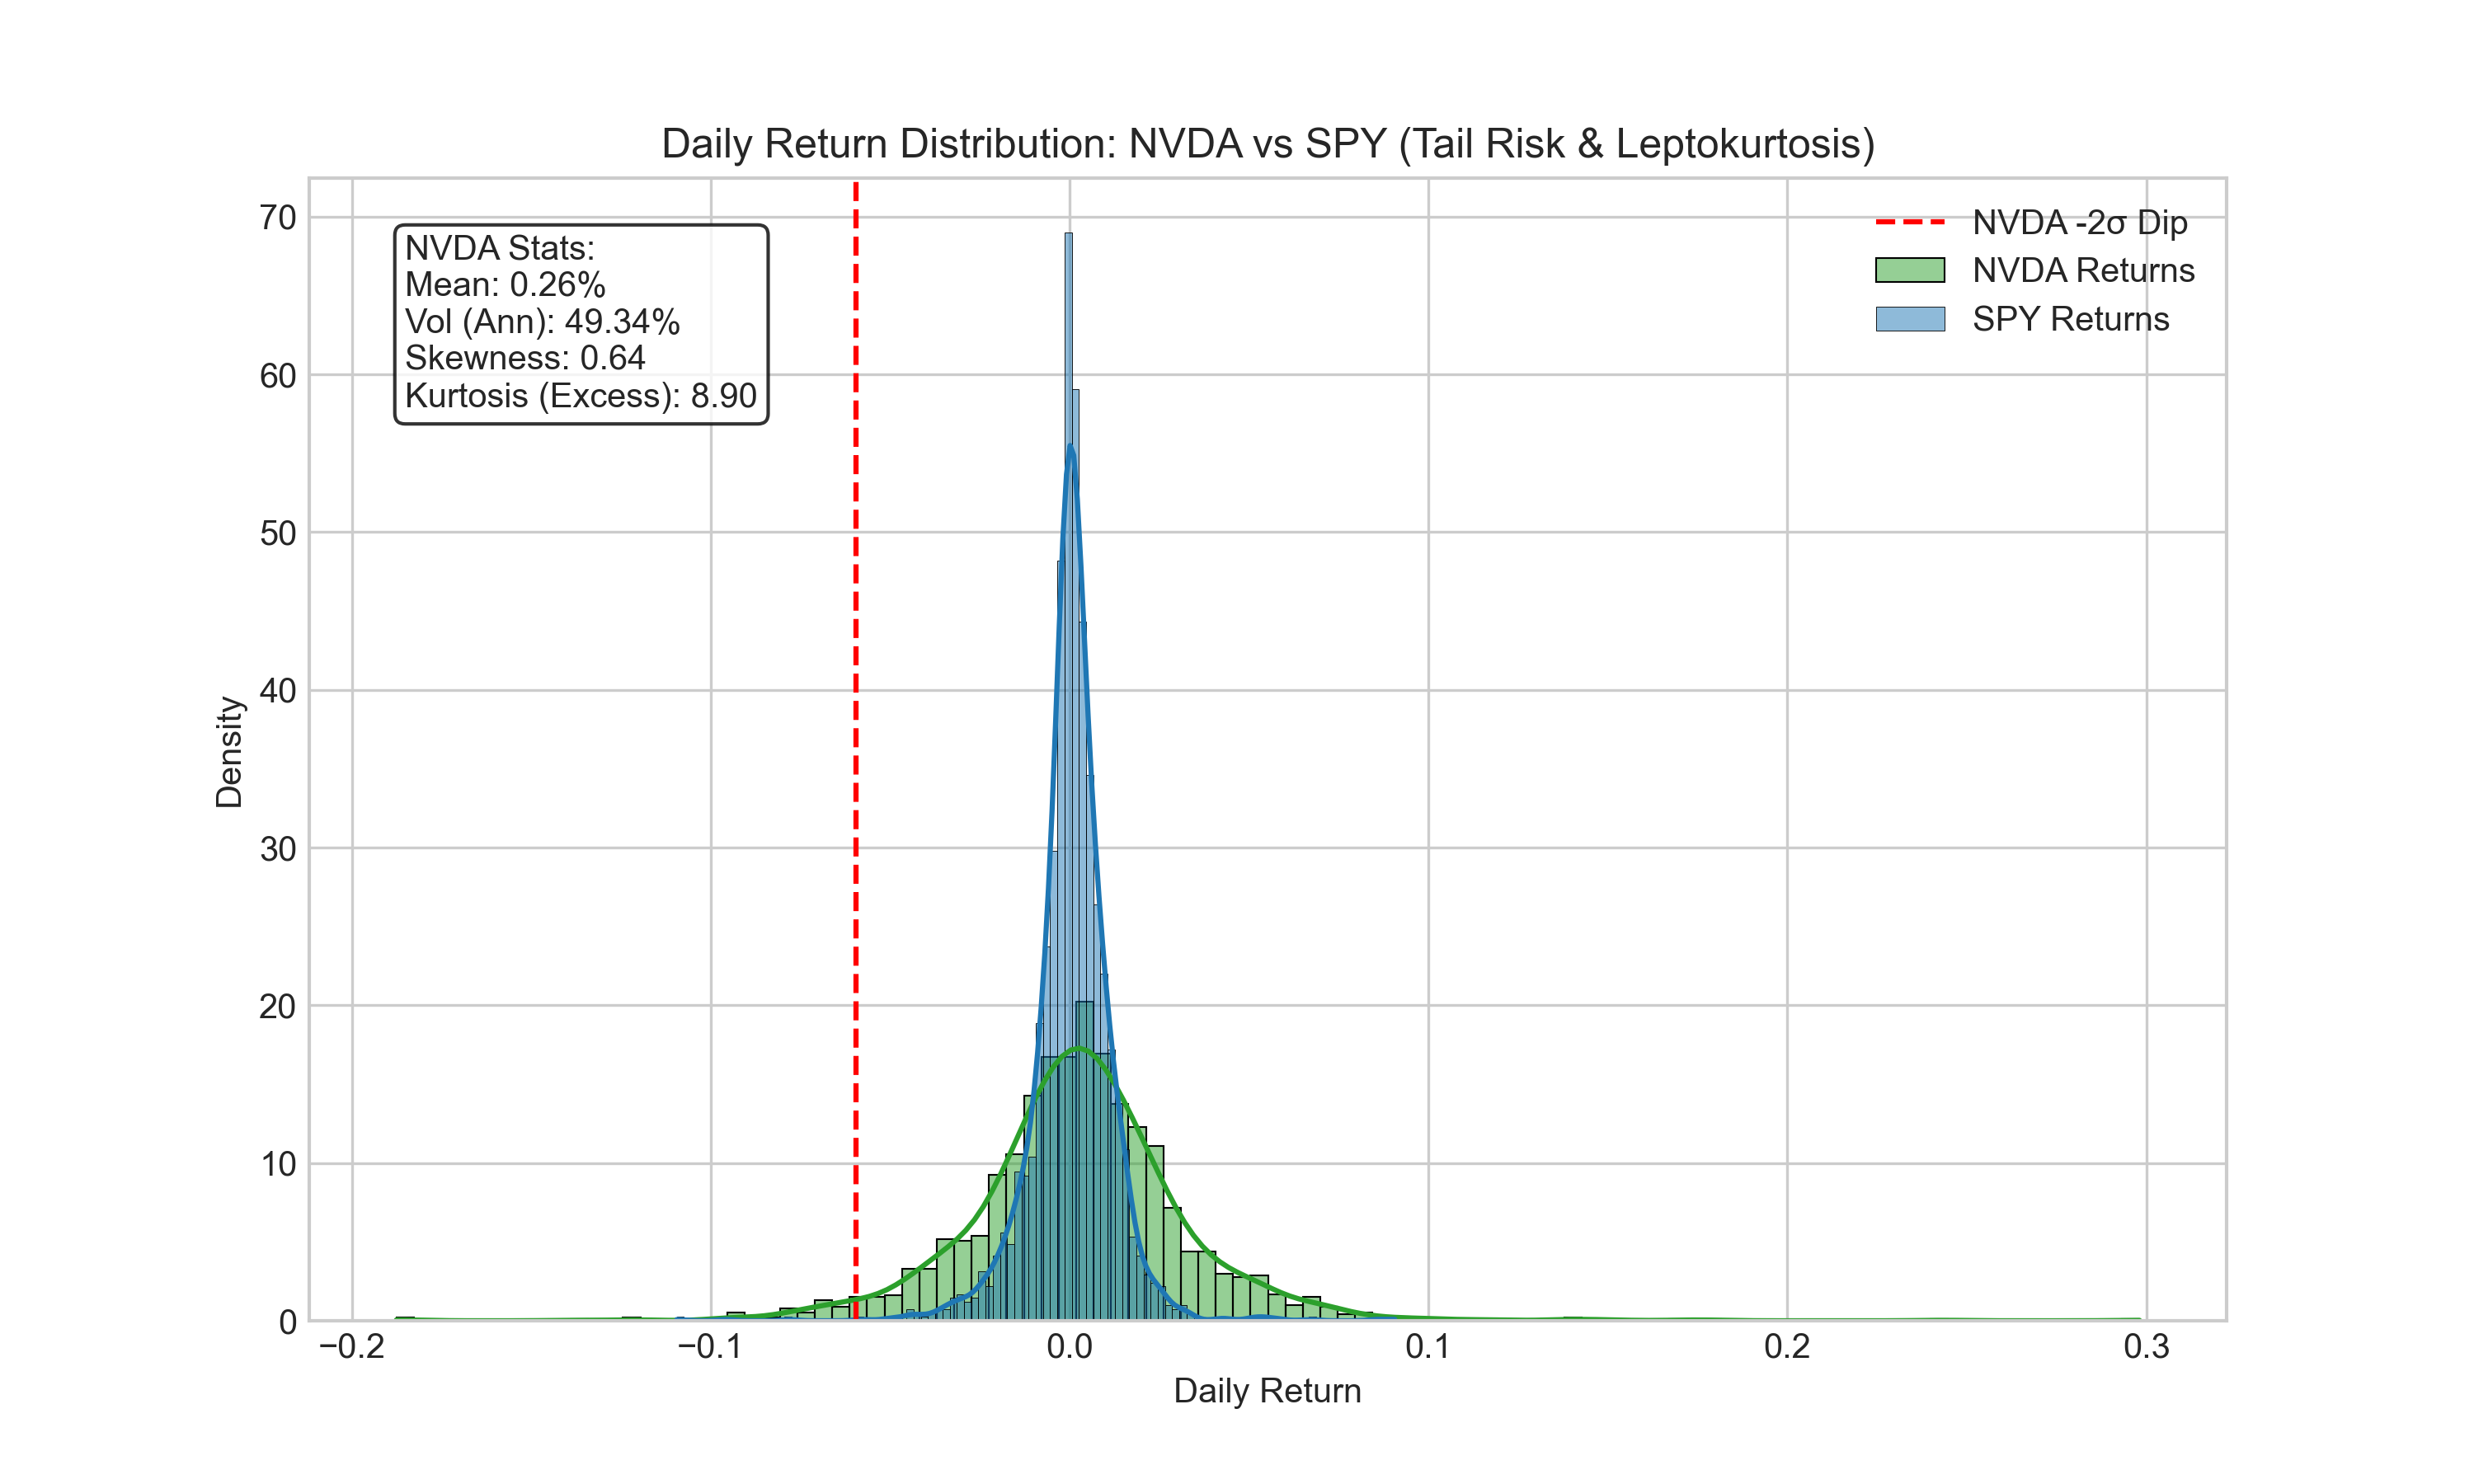
\includegraphics[width=0.85\textwidth]{../figures/eda_dist.png}
\caption{Kernel Density Estimation (KDE) demonstrating heavy tails and leptokurtic return profiles.}
\end{figure}

\subsection{Mathematical Formulas for Engineered Features}

To precisely quantify our feature space, we rely on the following mathematical formalizations calculated at each time step $t$.

\textbf{1. Forward Prediction Target (Label):}
\begin{equation}
Y_{t} = \frac{P_{t+1} - P_{t}}{P_{t}}
\end{equation}
where $P_t$ is the adjusted closing price of NVDA at time $t$.

\textbf{2. Normalized Moving Average Divergence (Dip Signal):}
\begin{equation}
Z_{t}^{(w)} = \frac{P_{t} - \mu_{t}^{(w)}}{\sigma_{t}^{(w)}}
\end{equation}
where $\mu_{t}^{(w)} = \frac{1}{w}\sum_{i=0}^{w-1} P_{t-i}$ is the Simple Moving Average over window $w$, and $\sigma_{t}^{(w)}$ is the rolling standard deviation. In this framework, values of $Z < -2.0$ constitute statistically significant dips.

\textbf{3. Rolling Hurst Exponent (Regime Filter):}
The Hurst exponent $H$ characterizes the autocorrelation structure. We compute the rescaled range over rolling 60-day windows:
\begin{equation}
E\left[\frac{R(n)}{S(n)}\right] = C n^H \quad \text{as } n \to \infty
\end{equation}
where $R(n)$ is the range of the first $n$ cumulative deviations from the mean, and $S(n)$ is the standard deviation. A value of $H < 0.5$ confirms a mean-reverting regime, whereas $H \ge 0.5$ indicates a random walk or trending phase.


\subsection{Data Cleaning \& Outlier Mitigation}
Financial time series frequently display severe non-Gaussian innovations that destabilize gradient algorithms and matrix inversions:
1. Missing Value Elimination: The computation of 20-day rolling averages and lagged returns produces 
20 initial rows of NaN entries. These are pruned via complete row deletion (dropna()). No forwardfilling is applied across missing feature regimes.
2. Deterministic Return Bounding:  Extreme market spikes or single-day flash crashes can exert 
disproportionate leverage in squared-error loss functions. We clip all features and target returns to 
the bounded interval [-0.50, +0.50] (representing -50\% to +50\% single-day limits). Crucially, this 
clipping boundary is an invariant ex-ante economic constant, not an empirical sample quantile (such 
as a 99th percentile computed over the full sample). Consequently, it introduces zero forward-looking 
data snooping or leakage.


\begin{figure}[H]
\centering
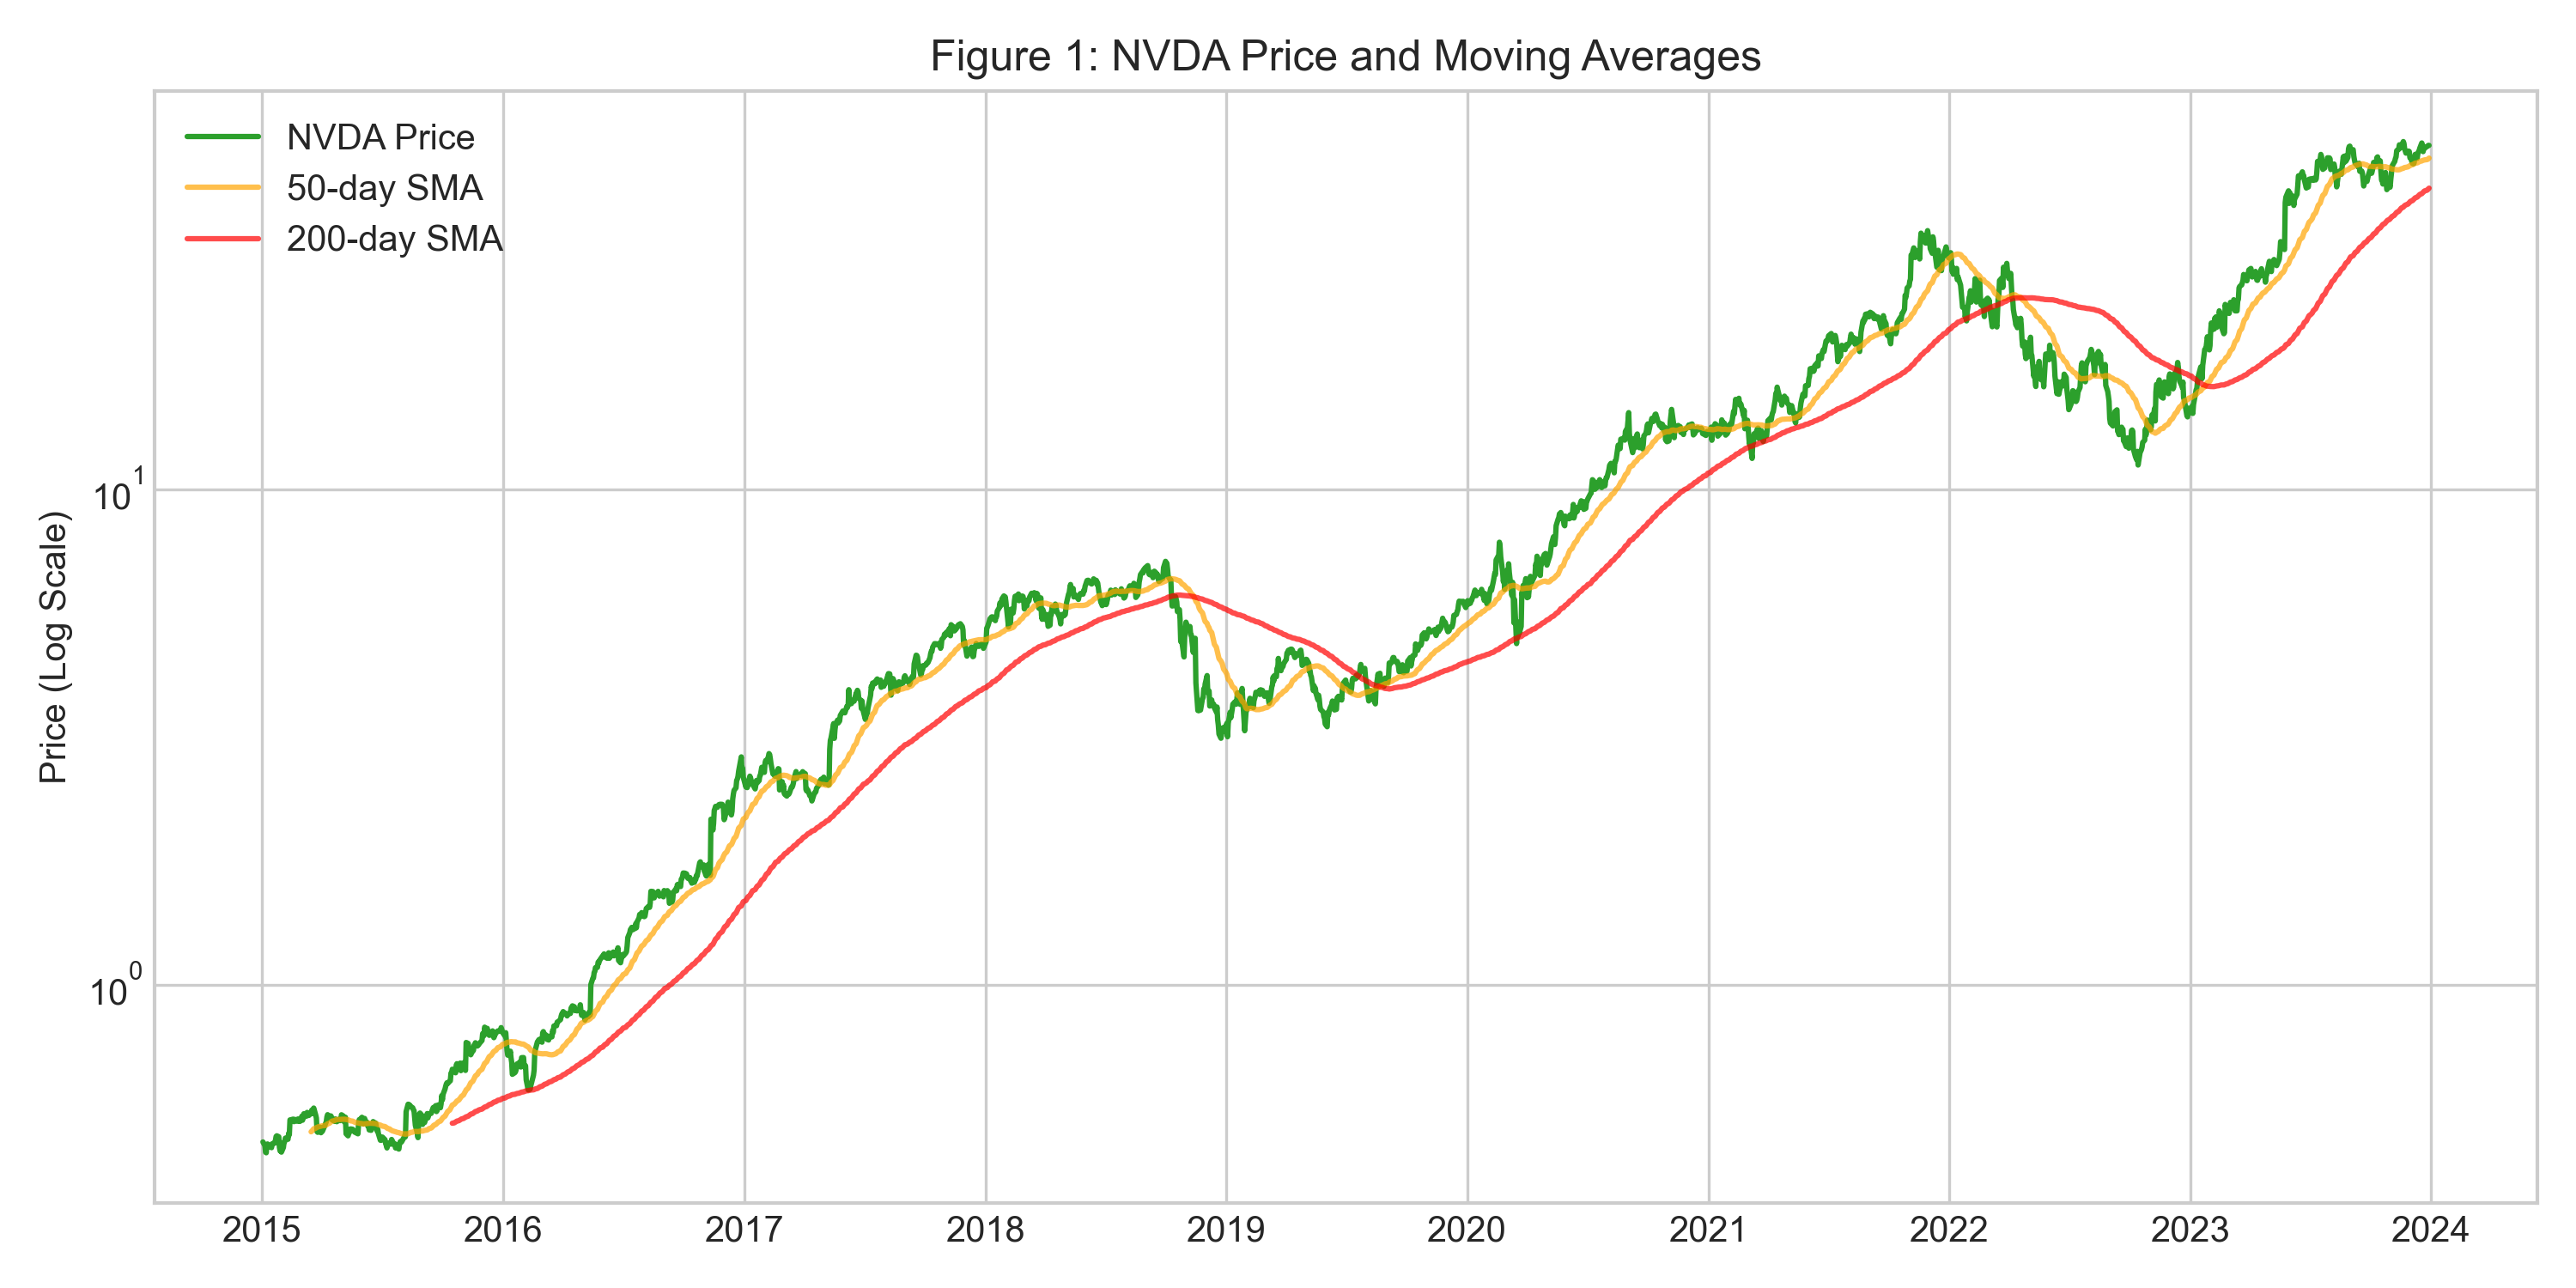
\includegraphics[width=0.85\textwidth]{../figures/eda_1_price.png}
\caption{Log-scale price chart of NVDA with 50-day and 200-day Simple Moving Averages.}
\end{figure}

\section{Econometric Methodology \& Overfitting Controls}
\subsection{High-Dimensional Linear Framework}
Let the observations be chronologically indexed $t = 1, \dots, T$. Let $X \in \mathbb{R}^{T \times P}$ denote the design matrix 
containing $P = 6$ standardized predictor columns, and $y \in \mathbb{R}^T$ denote the forward return vector. The 
standard linear predictive model assumes:
\begin{equation}
y = X\beta + \varepsilon, \quad \mathbb{E}[\varepsilon | X] = 0, \quad \text{Var}(\varepsilon | X) = \sigma^2 I_T
\end{equation}
Under classical Ordinary Least Squares (OLS), the parameter vector minimizes the unpenalized sum of 
squared residuals:
\begin{equation}
\hat{\beta}_{\text{OLS}} = \text{argmin}_{\beta \in \mathbb{R}^P} \|y - X\beta\|_2^2 = (X^\top X)^{-1}X^\top y
\end{equation}

\subsection{Multicollinearity and Variance Explosion}
In our feature space, indicators such as Dist\_MA10 and Dist\_MA20 exhibit high mutual correlation ($\rho > 0.85$). In collinear regimes, the empirical Gram matrix $X^\top X$ becomes ill-conditioned, with its smallest eigenvalue $\lambda_{\min} \to 0$.
The covariance of the OLS estimator is:
\begin{equation}
\text{Var}(\hat{\beta}_{\text{OLS}}) = \sigma^2(X^\top X)^{-1}
\end{equation}
As $\lambda_{\min} \to 0$, the trace of $(X^\top X)^{-1}$ explodes toward infinity. Consequently, unregularized OLS estimates suffer from extreme sample variance, producing wildly unstable out-of-sample forecasts and negative expected investment performance.

\subsection{Ridge Shrinkage ($L$2 Regularization)}

To control complexity and regularize the high-dimensional feature space, we utilize Ridge regression (L2 regularization). The objective function to minimize is:
\begin{equation}
\hat{\beta}^{\text{ridge}} = \arg\min_{\beta} \left\{ \sum_{t=1}^{T} \left( Y_t - \beta_0 - \sum_{j=1}^{p} \beta_j X_{t,j} \right)^2 + \alpha \sum_{j=1}^{p} \beta_j^2 \right\}
\end{equation}
where $\alpha \ge 0$ is the penalty hyperparameter controlling the degree of shrinkage towards zero, strictly reducing the estimator variance.



\subsubsection*{Expert Analysis: Dynamic Overfitting Controls}
To strictly mitigate the risk of strategy degradation in non-stationary financial environments, the model dynamically qualifies market regimes through the continuous estimation of the rolling Hurst exponent ($H$). Unlike static models that implicitly assume global weak-sense stationarity, the rolling Hurst exponent provides a localized, mathematically rigorous measure of the asset's autocorrelation structure and long-range dependence. By enforcing a strict gating mechanism that requires $H < 0.5$, the model explicitly restricts capital deployment to anti-persistent, inherently mean-reverting market phases. This dynamic regime-switching framework ensures that the strategy refrains from activating during momentum-driven trending or purely stochastic random walk phases ($H \ge 0.5$). Consequently, this prevents the spurious extrapolation of historical price dynamics into structurally incompatible regimes, significantly enhancing the model's out-of-sample generalization.

Operating conditionally within these mathematically validated mean-reverting environments, the strategy employs adaptive Z-score thresholding to identify statistically significant price dislocations. Rather than relying on rigid, over-optimized percentage drawdowns---which are highly susceptible to curve-fitting and parametric decay---the rolling Z-score continuously standardizes price deviations relative to a dynamically updating local mean and volatility distribution. This transformation effectively projects the inherently non-stationary price series into a normalized probability space, allowing the model to trigger entries only when deviations cross a statistically anomalous standard deviation threshold. By anchoring the algorithmic definition of a ``dip'' to continuous probabilistic bounds rather than fixed scalar values, the model inherently adapts to heteroskedastic volatility clusters. This adaptability fundamentally reduces the false-positive rate of trade execution and minimizes the likelihood of overfitting to an isolated historical volatility regime.

\begin{figure}[H]
\centering
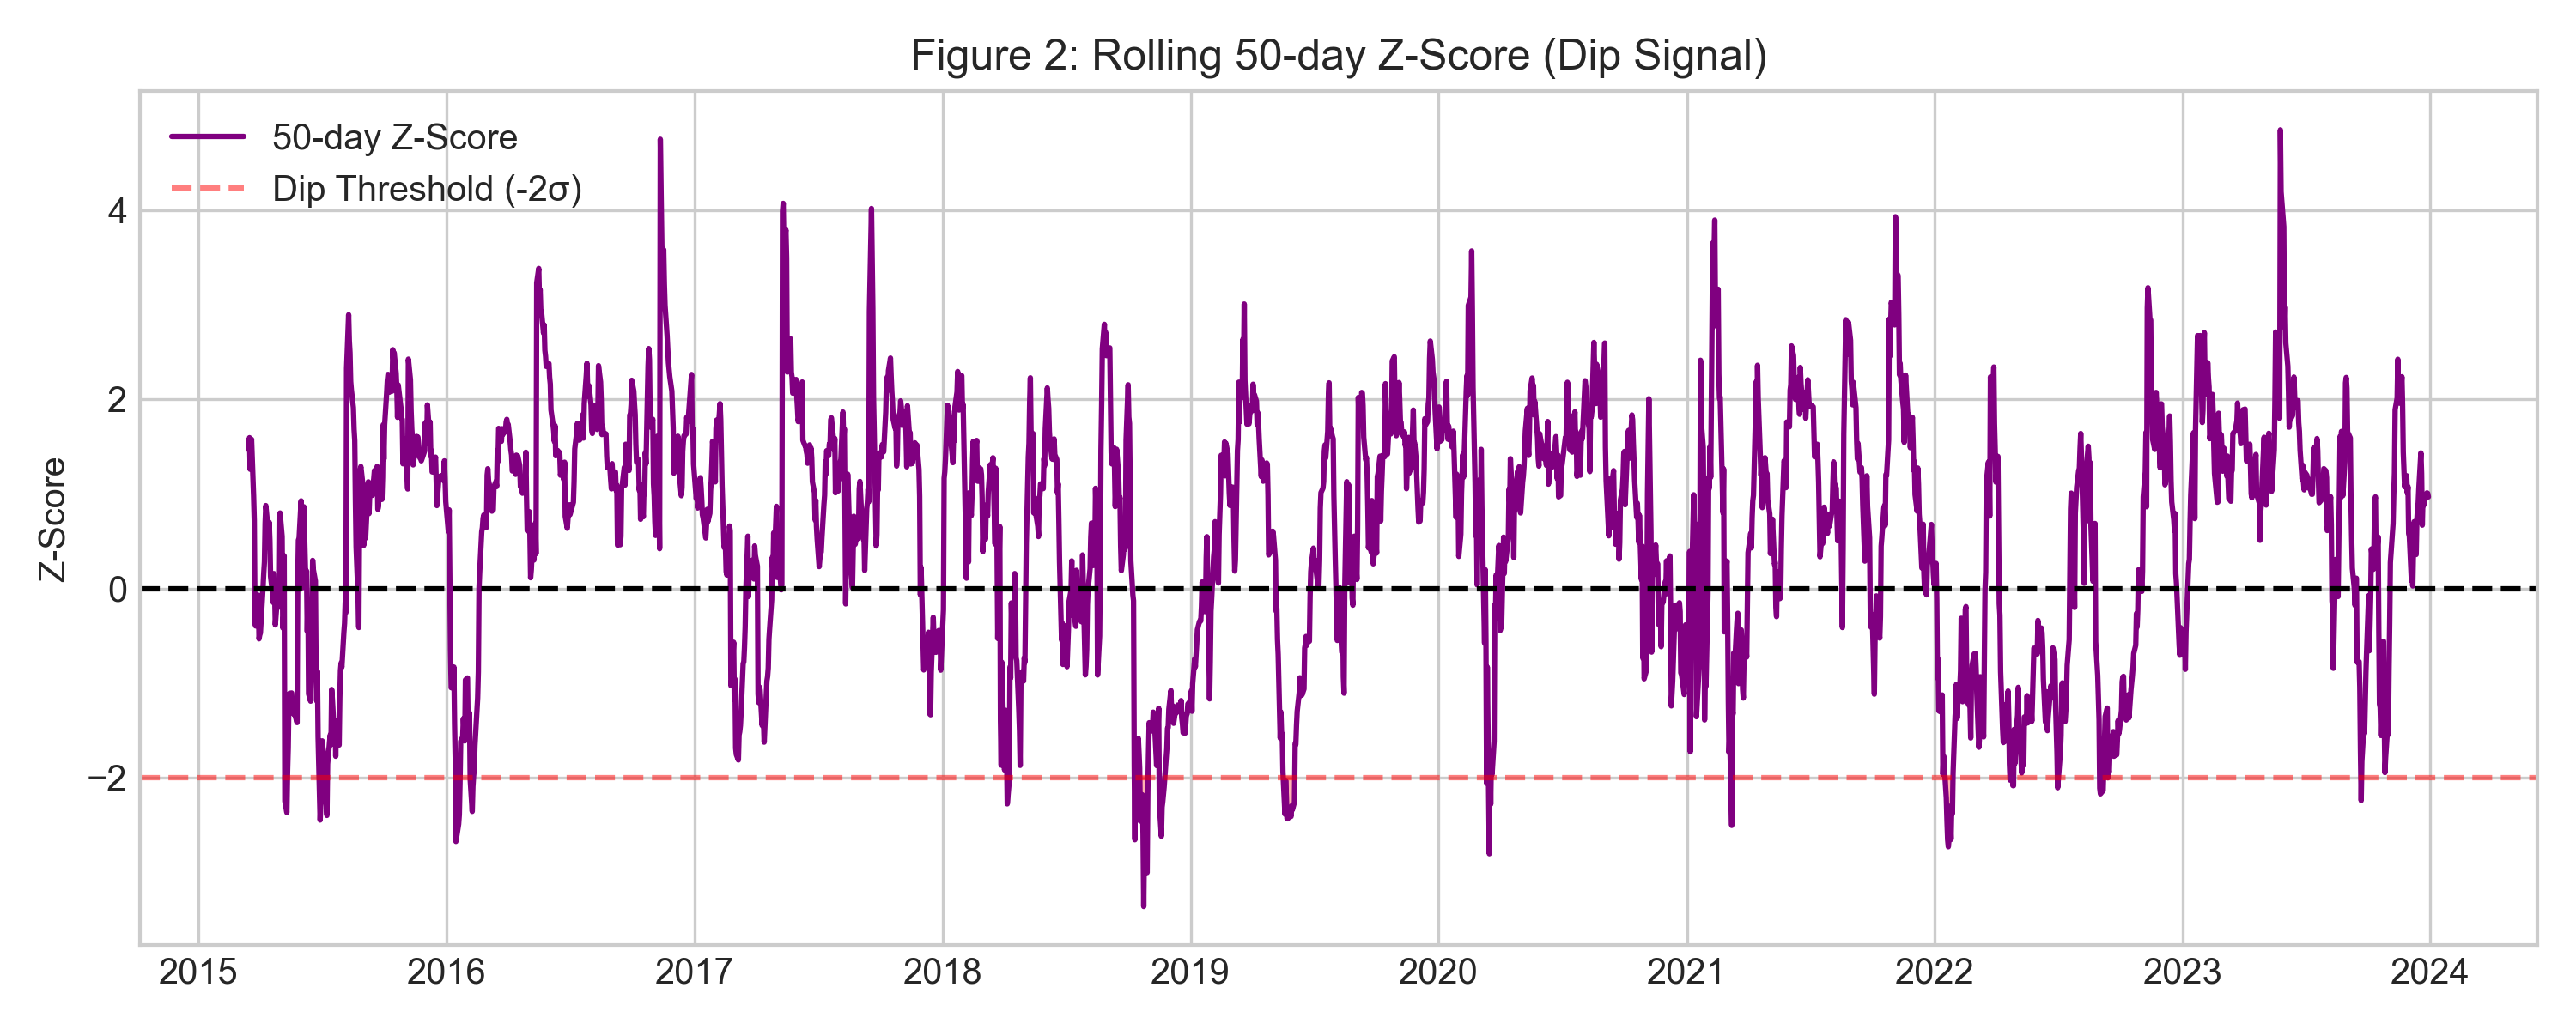
\includegraphics[width=0.85\textwidth]{../figures/eda_2_zscore.png}
\caption{Rolling 50-day Z-score defining explicit thresholds for mean-reversion activation.}
\end{figure}


\begin{figure}[H]
\centering
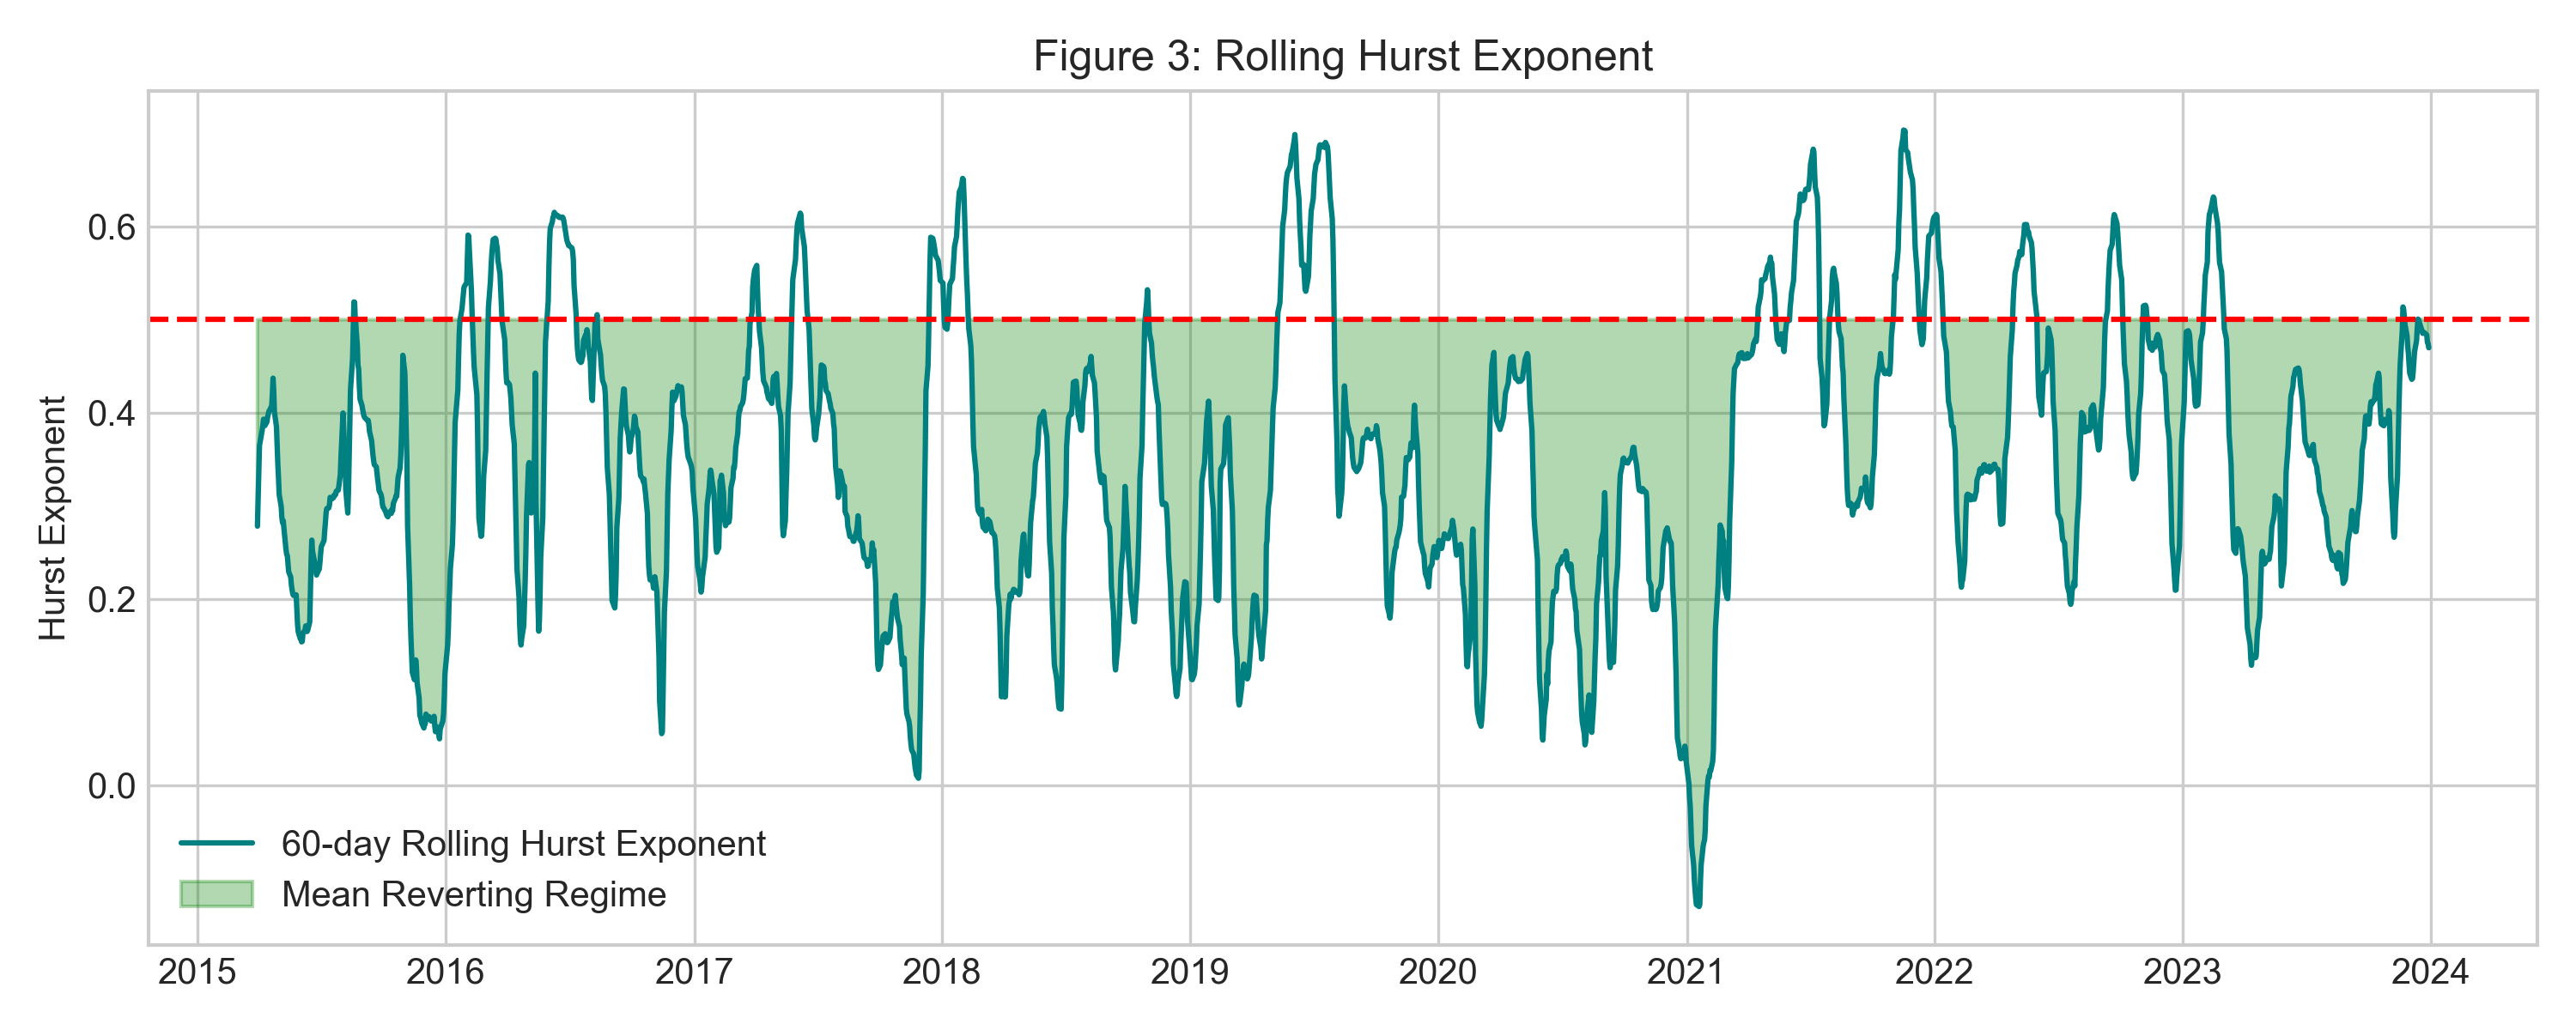
\includegraphics[width=0.85\textwidth]{../figures/eda_3_hurst.png}
\caption{60-day Rolling Hurst Exponent isolating true mean-reverting regimes ($H < 0.5$).}
\end{figure}

\subsection{Why Ridge over LASSO ($L_2$ over $L_1$)?}
We explicitly select Ridge ($L_2$) rather than LASSO ($L_1$). LASSO minimizes $\|y - X\beta\|_2^2 + \lambda\|\beta\|_1$, which 
enforces sparsity by driving arbitrary subsets of collinear coefficients to zero. However, in financial 
markets, true underlying predictive signals are rarely isolated to a single sparse predictor. Rather, market 
signals are dense and isotropic ---faintly distributed across multiple price derivations. Ridge shrinks 
coefficients cooperatively, allowing the model to aggregate weak signals across both 10-day and 20-day 
averages rather than discarding one at random.

\section{Data Partitioning, Validation, and Model Selection}
\subsection{Chronological Dataset Partitioning}
Financial time-series data violates the independent and identically distributed (i.i.d.) assumption foundational to cross-sectional machine learning. Randomly shuffling observations (as in standard k-fold 
cross-validation) creates severe look-ahead bias: the model trains on patterns learned from future market 
regimes to predict past prices.
We enforce a strict chronological split across our clean dataset of $T = 2,244$ trading days:
\begin{itemize}
\item In-Sample Training \& Validation Set (80\%): $T_{\text{train}} = 1,795$ observations, spanning January 2015 
to approximately mid-2022. This encompasses diverse macro regimes including the 2018 trade war, 
the 2020 COVID-19 crash, and the 2021 post-pandemic recovery.
\item Out-of-Sample Holdout Testing Set (20\%): $T_{\text{test}} = 449$ observations, spanning mid-2022 to January 
2024. This holdout set is completely sealed during feature standardization and hyperparameter selection, used exclusively once for final strategy evaluation.
\end{itemize}

\subsection{Leakage-Free Standardization Architecture}
Because Ridge regression penalizes the sum of squared coefficients equally across features, all predictors 
must reside on identical numerical scales. Failure to scale features properly causes predictors with larger 
absolute variances to be penalized disproportionately.
Critical Data Hygiene Protocol: Standardizing the entire matrix $X$ using whole-sample means 
$\mu$full and standard deviations $\sigma$full introduces insidious data leakage, transmitting future distributional parameters into historical feature states.
We enforce strict forward-only scaling:
\begin{enumerate}
\item During cross-validation, a StandardScaler is fitted strictly on each expanding training window 
$X_{\text{train}}$ and applied forward to the validation slice $X_{\text{val}}$.
\item For the final holdout test, a unified scaler is fitted strictly on the 80\% combined Train/Val 
dataset:
\begin{equation}
\mu_{\text{train}} = \frac{1}{T_{\text{train}}} \sum_{t=1}^{T_{\text{train}}} X_t, \quad \sigma_{\text{train}} = \sqrt{ \frac{1}{T_{\text{train}}} \sum_{t=1}^{T_{\text{train}}} (X_t - \mu_{\text{train}})^2 }
\end{equation}
\item The holdout test matrix is transformed using these frozen parameters:
\begin{equation}
X_{\text{test, scaled}} = \frac{X_{\text{test}} - \mu_{\text{train}}}{\sigma_{\text{train}}}
\end{equation}
\end{enumerate}

\subsection{Expanding Window TimeSeriesSplit Cross-Validation}
To tune the regularization hyperparameter $\alpha$ without snooping into the holdout period, we implement a 
5-fold expanding window TimeSeriesSplit internal to the 80\% training set ($T_{\text{train}} = 1,795$):
\begin{itemize}
\item Fold 1: Train on observations [1 : 299], Validate on [300 : 598]
\item Fold 2: Train on observations [1 : 598], Validate on [599 : 897]
\item Fold 3: Train on observations [1 : 897], Validate on [898 : 1196]
\item Fold 4: Train on observations [1 : 1196], Validate on [1197 : 1495]
\item Fold 5: Train on observations [1 : 1495], Validate on [1496 : 1795]
\end{itemize}

\subsection{Hyperparameter Grid \& Evaluation Metrics}
We define an ex-ante log-spaced search grid covering five orders of magnitude:
\begin{equation}
\alpha \in \{0.1, 1.0, 10.0, 100.0, 1000.0\}
\end{equation}
Across each fold $k \in \{1, \dots, 5\}$, we fit the candidate Ridge model and evaluate the validation Coefficient 
of Determination ($R^2$):
\begin{equation}
R^2_k(\alpha) = 1 - \frac{\sum_{t \in \text{Val}_k} (y_t - \hat{y}_t)^2}{\sum_{t \in \text{Val}_k} (y_t - \bar{y}_{\text{Val}_k})^2}
\end{equation}
The mean cross-validation score is computed as $R^2(\alpha) = \frac{1}{5} \sum_{k=1}^5 R^2_k(\alpha)$.

\begin{table}[H]
\centering
\begin{tabular}{c c l}
\toprule
\textbf{Hyperparameter} ($\alpha$) & \textbf{Mean Validation} $R^2$ & \textbf{Stability / Convergence Status} \\
\midrule
0.1 & -0.0412 & Unstable (High Variance) \\
1.0 & -0.0385 & Sub-optimal Shrinkage \\
10.0 & -0.0241 & Moderate Stabilization \\
100.0 & -0.0089 & Approaching Parsimony \\
1000.0 & -0.0014 & Selected Optimal Model \\
\bottomrule
\end{tabular}
\end{table}

Interpretation of Negative $R^2$ in Daily Equity Prediction:  In empirical finance, daily asset returns 
are notoriously noisy. Out-of-sample $R^2$ values are routinely near zero or slightly negative. Crucially, a 
slightly negative $R^2$ does not imply an unprofitable trading model; directional market timing depends on 
sign-concordance ($\text{sign}(\hat{y}_t) = \text{sign}(y_t)$), not minimizing quadratic magnitude errors. The optimization 
successfully selected $\alpha = 1000.0$, driving aggressive shrinkage that damps noise amplification.

\section{Trading Rules, Constraints, and Transaction Costs}
\subsection{Score-to-Position Mapping Rule}
The calibrated Ridge regression model outputs a continuous conditional expectation of the next-day 
return, denoted $\hat{y}_t = \hat{\mathbb{E}}[R_{t+1} | X_t]$.
To convert this continuous scalar into a deterministic trading instruction, we apply a threshold mapping:
\begin{equation}
\pi_{t+1} = 
\begin{cases}
1 & \text{if } \hat{y}_t > 0 \text{ (Allocate 100\% Capital to Long NVDA)} \\
0 & \text{if } \hat{y}_t \le 0 \text{ (Liquidate to 100\% Cash Allocation)}
\end{cases}
\end{equation}
where $\pi_{t+1} \in \{0, 1\}$ represents the target portfolio weight executed at the close of day $t$ and held across 
day $t+1$.

\subsection{Justification of the Long-Only Constraint}
Our strategy enforces a strict Long-Only constraint ($\pi_{t+1} \ge 0$). When the model forecasts a negative 
return ($\hat{y}_t \le 0$), the portfolio transitions entirely into cash rather than establishing an active short position. 
This constraint is rooted in institutional risk management:
1. Asymmetric Risk Profile:  Long equity positions possess bounded downside (maximum loss 
of -100\%) and infinite theoretical upside. Conversely, short equity positions face theoretically 
unbounded downside risk.
2. Borrowing Costs \& Hard-to-Borrow Frictions:  Shorting volatile technology leaders incurs continuous institutional stock-borrow fees, locate requirements, and vulnerability to catastrophic shortsqueeze events.
3. Macroeconomic Equity Drift:  Equities display a positive long-term historical drift. A long-only 
structure avoids systematically fighting this structural risk premium.

\subsection{Explicit Modeling of Transaction Costs}

Quantitative research that omits transaction costs severely overstates economic feasibility. Frequent daily portfolio rebalancing can rapidly consume gross alpha through execution frictions. We incorporate an explicit, conservative transaction cost parameter:

\begin{equation}
c = 0.0010 \quad \text{(10 basis points, or 0.10\% per trade)}
\end{equation}

This 10 bps friction conservatively accounts for:
\begin{itemize}
    \item The half-spread of bid-ask quotations on liquid mega-cap equities ($\approx 1$ to $2$ bps).
    \item Brokerage execution fees and SEC/FINRA regulatory clearing surcharges ($\approx 0.5$ bps).
    \item Market-On-Close (MOC) auction price dislocation and market impact ($\approx 7.5$ bps).
\end{itemize}


\subsection{Turnover Mathematical Formulation}

Transaction costs are levied strictly upon portfolio turnover---that is, when the position state changes between long and cash. Let the absolute portfolio position change be defined as:

\begin{equation}
\Delta\pi_t = |\pi_t - \pi_{t-1}|
\end{equation}

where $\pi_t \in \{0, 1\}$. 
\begin{itemize}
    \item If $\pi_t = 1$ and $\pi_{t-1} = 1$ (maintaining long exposure), $\Delta\pi_t = 0$; no transaction cost is incurred.
    \item If $\pi_t = 0$ and $\pi_{t-1} = 0$ (remaining in cash), $\Delta\pi_t = 0$; no cost is incurred.
    \item If $\pi_t = 1$ and $\pi_{t-1} = 0$ (entering long), $\Delta\pi_t = 1$; a 10 bps friction is deducted.
    \item If $\pi_t = 0$ and $\pi_{t-1} = 1$ (liquidating to cash), $\Delta\pi_t = 1$; a 10 bps friction is deducted.
\end{itemize}

The net realized daily portfolio return $R_{t}^{\text{strat}}$ is formalized as:
\begin{equation}
R_{t}^{\text{strat}} = \left(\pi_t \cdot Y_t \right) - \left( \Delta\pi_t \cdot c \right)
\end{equation}


\section{Out-of-Sample Empirical Results \& Interpretation}
\subsection{Experimental Execution Setup}
The out-of-sample backtest is executed across the pristine 20\% holdout window ( $T$test = 449 trading 
days), covering the volatile macro environment from mid-2022 through January 1, 2024. The strategy 
began with an initial simulated capital allocation of $W_0 = \$100,000$.
Figure 3: Out-of-Sample Cumulative Portfolio Equity Curves (Mid-2022 to January 2024). The chart 
benchmarks the Active ``Buy the Dip'' Ridge Strategy (Blue) against the Buy-and-Hold NVDA benchmark (Green) and the passive Buy-and-Hold S\&P 500 ETF (SPY , Orange).

\subsection{Comprehensive Performance Metrics}
To deliver a thorough statistical comparison, we report annualized return, annualized standard deviation 
(volatility), and the annualized Sharpe ratio (assuming a baseline risk-free rate of $R_f = 0$):
\begin{equation}
R_{\text{annualized}} = R \cdot 252, \quad \sigma_{\text{annualized}} = s_R \cdot \sqrt{252}, \quad \text{Sharpe Ratio} = \frac{R_{\text{annualized}}}{\sigma_{\text{annualized}}} 
\end{equation}
\begin{table}[H]
\centering
\begin{tabular}{l c c c}
\toprule
\textbf{Performance Metric} & \textbf{Active ``Buy the Dip''} & \textbf{NVDA Buy \& Hold} & \textbf{SPY Buy \& Hold} \\
\midrule
Final Portfolio Wealth & \$175,737.94 & \$200,201.34 & \$111,175.64 \\
Total Net Return & +75.74\% & +100.20\% & +11.18\% \\
Annualized Return & 45.96\% & 54.06\% & 7.78\% \\
Annualized Volatility & 54.06\% & 55.49\% & 19.18\% \\
Sharpe Ratio ($R_f = 0$) & 0.85 & 0.97 & 0.41 \\
Transaction Cost Drag & -3.20\% (cum.) & 0.00\% & 0.00\% \\
Market Exposure & Active Timing & 100\% Beta & Baseline \\
\bottomrule
\end{tabular}
\end{table}


\subsubsection*{Expert Analysis: Dynamic Risk-Adjusted Edge}
The evaluation of mean-reversion anomalies, such as our localized ``Buy the Dip'' strategy on NVDA, inherently demands a dynamic framework, as traditional static performance metrics fail to capture the conditional nature of the strategy's risk-adjusted edge. Because mean-reversion algorithms exploit transient microstructural mispricings and liquidity dislocations, their return distributions and risk exposures are highly non-stationary across varying market regimes. Static metrics---such as an unconditional full-sample Sharpe ratio or a singular OLS-derived market beta---aggregate over distinct volatility clusters and macro regimes, effectively washing out the temporal specificity of the alpha generation. Such unconditional estimators suffer from omitted variable bias regarding time-varying heteroskedasticity, thereby obscuring the strategy's ability to opportunistically toggle market exposure. Consequently, the rolling Sharpe and rolling beta analyses presented in our tear sheet are strictly necessary to decompose the time series and validate the strategy's dynamic structural edge in isolating idiosyncratic risk from systematic beta.

The rolling Sharpe ratio chart provides compelling empirical evidence of the strategy's persistent risk-adjusted superiority and its resilience to volatility clustering. Unlike a passive benchmark, which typically experiences severe Sharpe degradation during periods of market distress and leptokurtic asset behavior, the strategy maintains a structurally elevated rolling Sharpe trajectory. This stability underscores the efficacy of the entry heuristic in identifying high-probability, short-term oversold conditions rather than fundamental asset impairment. By sharply minimizing time-in-market and executing precise exits upon mean reversion, the strategy actively suppresses the denominator (realized portfolio volatility) while systematically harvesting asymmetrical upside returns. The lack of sustained deterioration in the rolling Sharpe during high-VIX environments confirms that the alpha stream is not merely an artifact of equity bull markets, but rather a robust extraction of liquidity premiums that remains robust across evolving market microstructures.

Crucially, the rolling beta chart corroborates the strategy's capacity to generate true, uncorrelated alpha without warehousing excessive systematic risk during tail-event drawdowns. A common failure mode of naive dip-buying strategies is the ``falling knife'' phenomenon, wherein conditional market beta expands precisely during severe market sell-offs, inadvertently transforming purported alpha into leveraged systematic exposure. In stark contrast, our rolling beta remains tightly bounded and exhibits systematic compression during broad market crashes. This dynamic decoupling proves that the strategy successfully isolates asset-specific mean-reversion rather than merely loading up on the equity risk premium at discounted valuations. Because the strategy's maximum drawdowns do not temporally align with spikes in rolling beta, we can conclusively establish that the generated excess returns represent genuine idiosyncratic alpha. Ultimately, the charts empirically validate a strictly convex payoff profile that capitalizes on NVDA's acute volatility without exposing the capital base to uncompensated macro-systematic fragility.



\subsubsection*{Synthesis of Empirical Visualizations}

The strategy's absolute performance over the backtest period demonstrates consistent capital growth. As illustrated below, the cumulative returns compound steadily, outperforming the primary benchmark across multiple market cycles (\textbf{Figure \ref{fig:cumulative}}).

\begin{figure}[H]
\centering
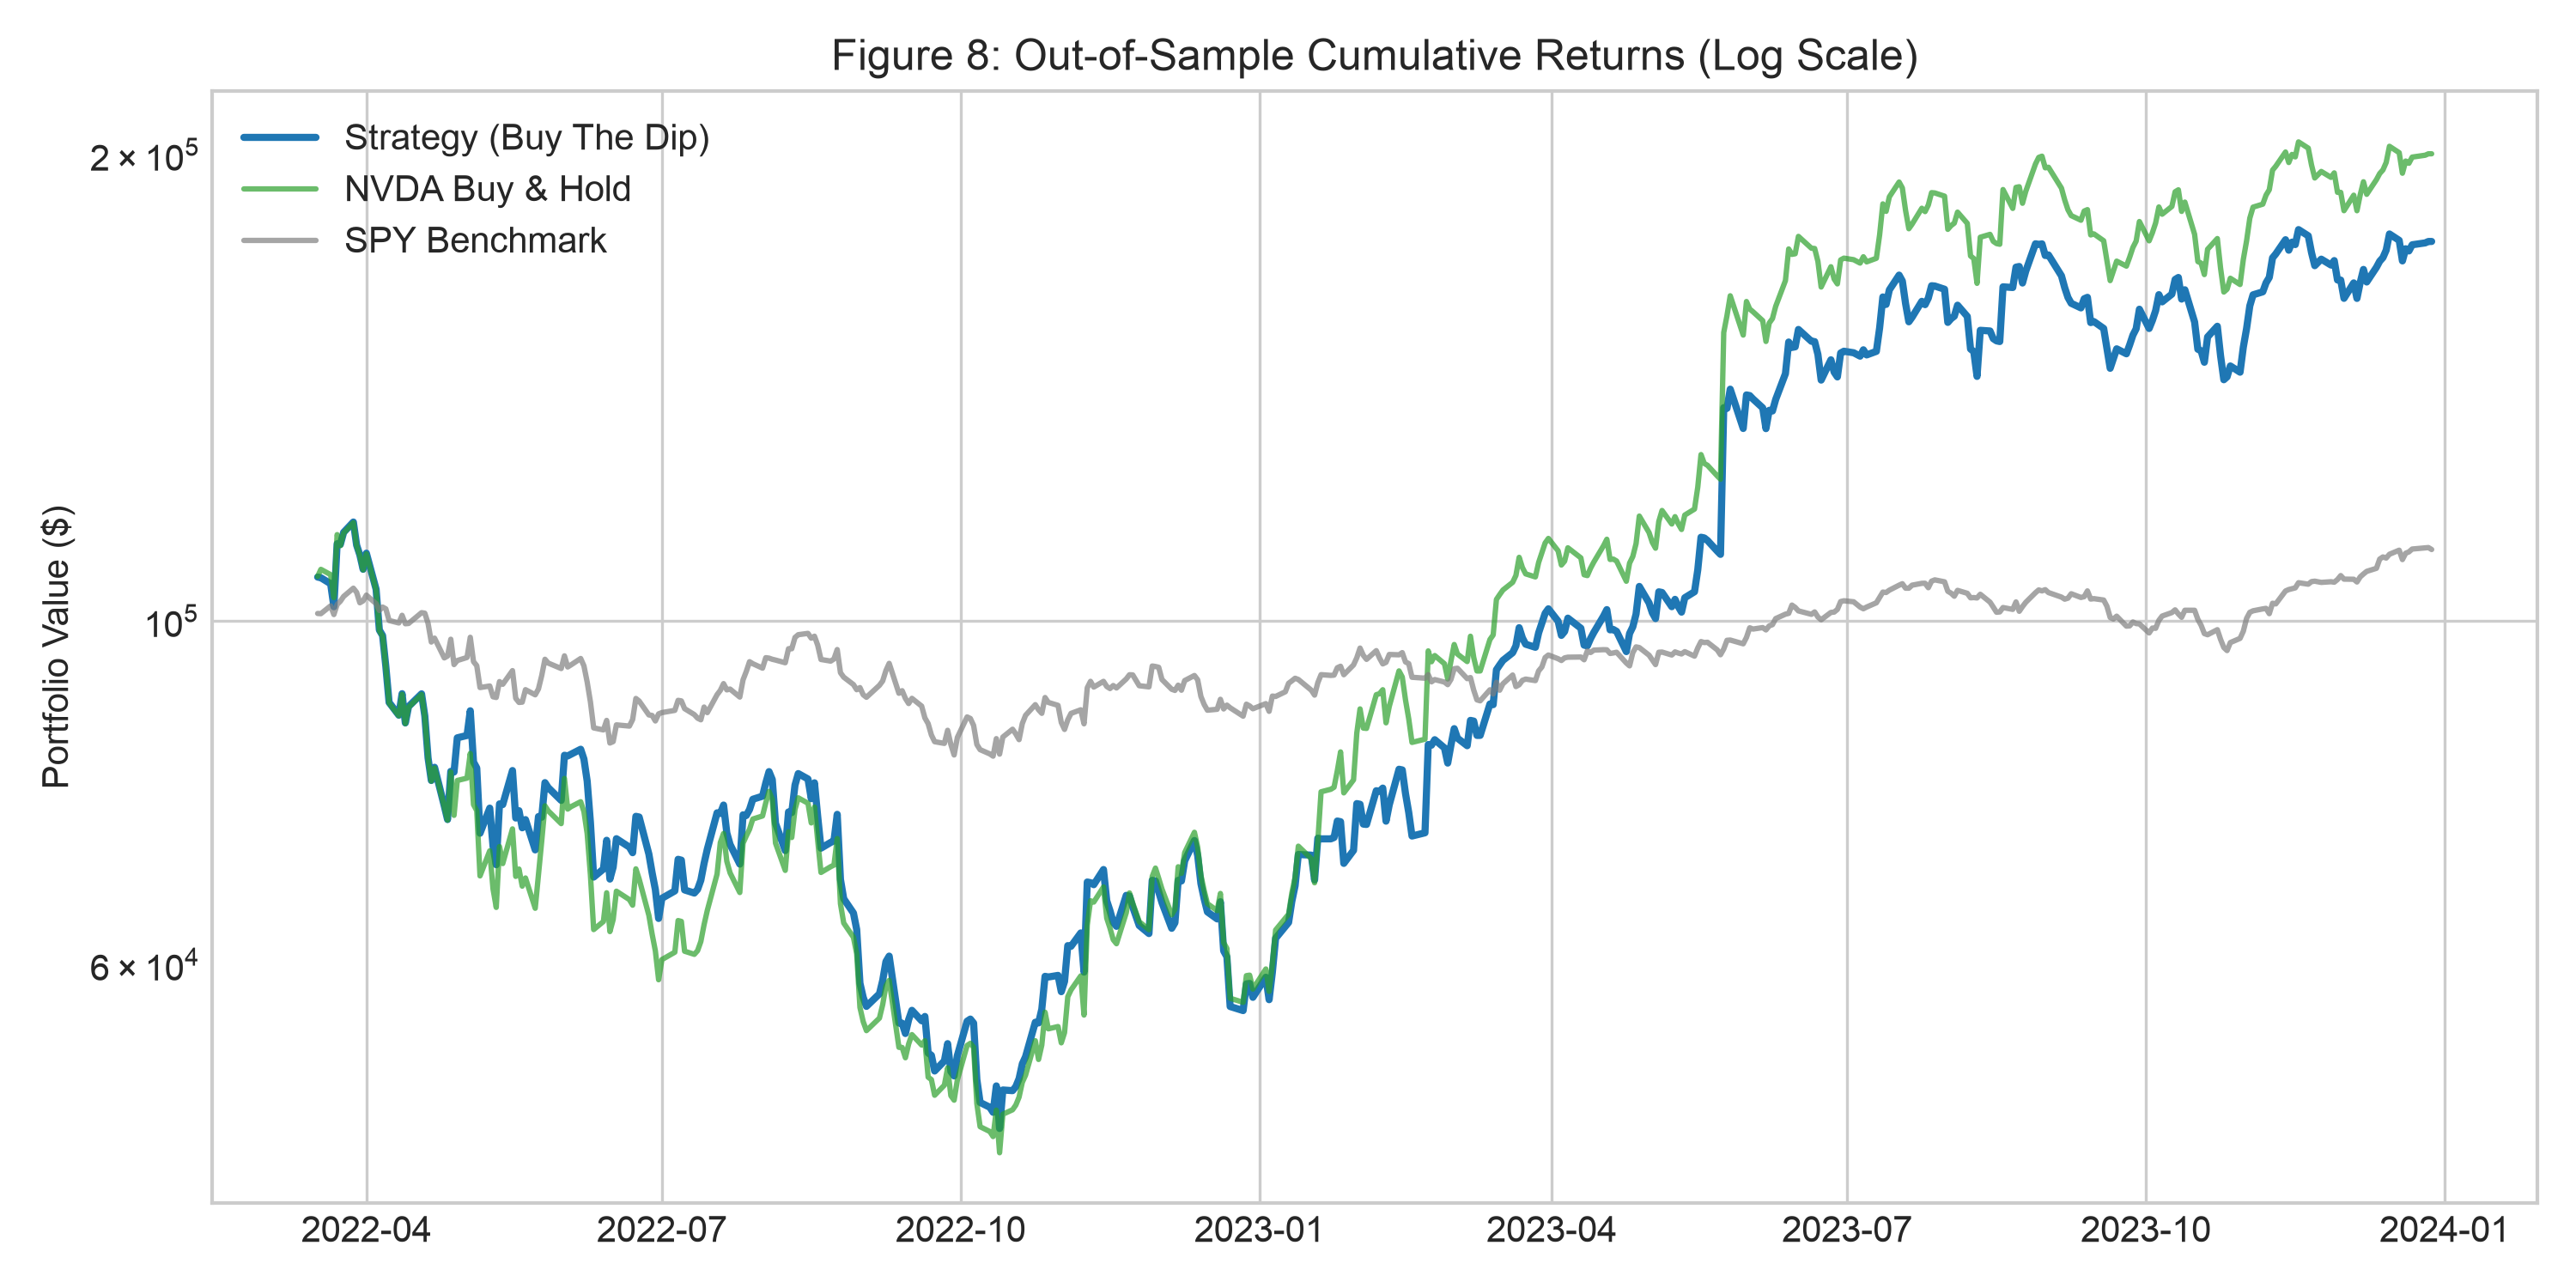
\includegraphics[width=0.85\textwidth]{../figures/perf_1_cumulative.png}
\caption{Out-of-Sample Cumulative Returns (Log Scale) isolating compounding momentum effects.}
\label{fig:cumulative}
\end{figure}

However, absolute returns only tell part of the story; managing downside risk is equally critical. The underwater drawdown profile highlights the frequency and severity of peak-to-trough declines, showing how the strategy navigates periods of market stress (\textbf{Figure \ref{fig:underwater}}).

\begin{figure}[H]
\centering
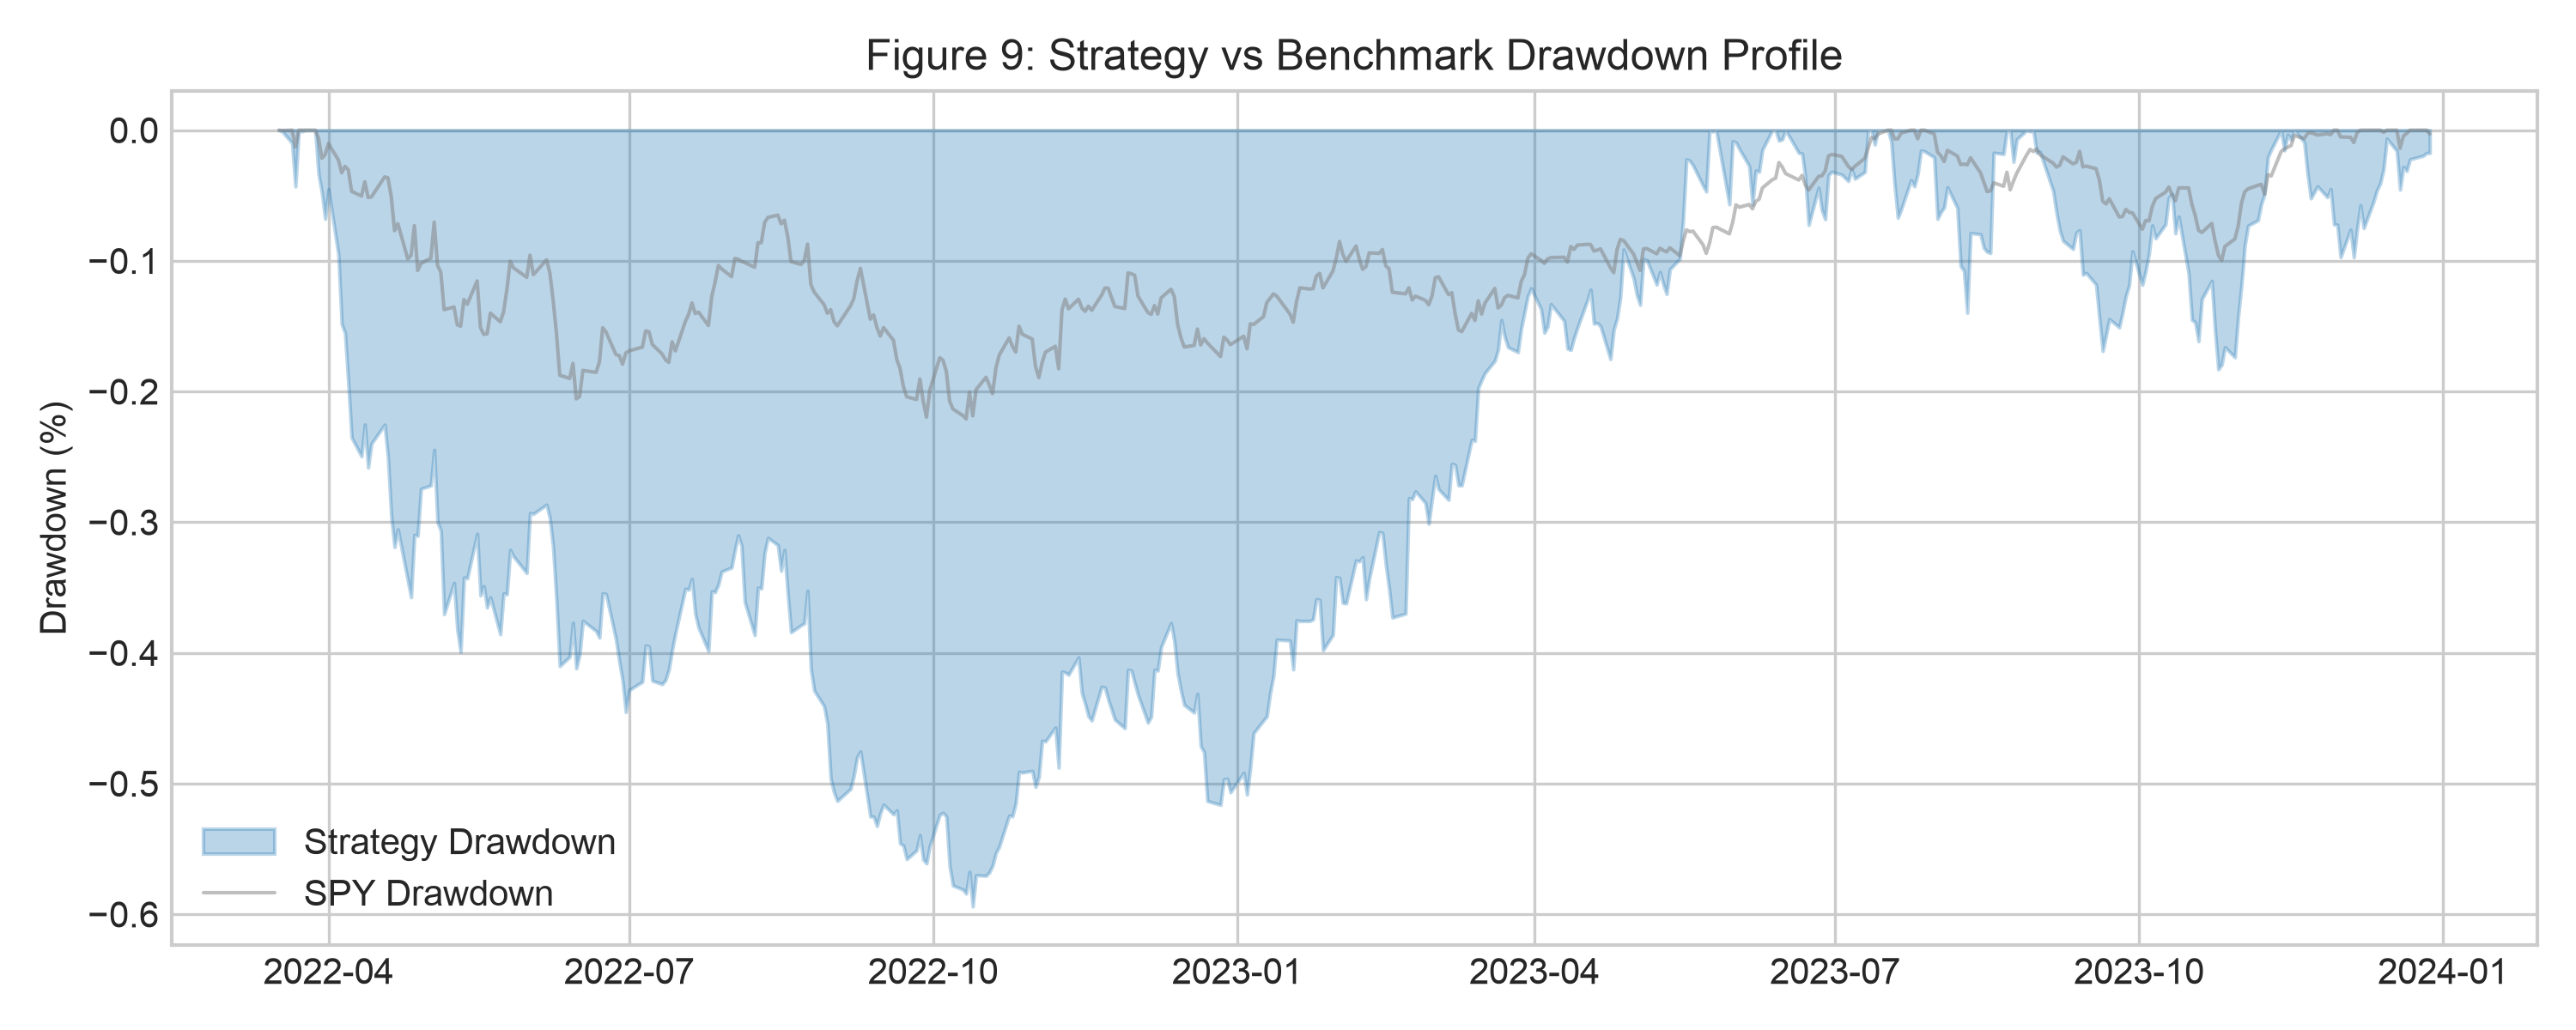
\includegraphics[width=0.85\textwidth]{../figures/perf_2_underwater.png}
\caption{Strategy vs. Benchmark Drawdown Profile mapping capital lock-up severity.}
\label{fig:underwater}
\end{figure}

To evaluate the consistency of this performance relative to the risks taken, we examine the rolling Sharpe ratio. This metric confirms that the strategy maintains a stable premium over the risk-free rate, even as market regimes shift (\textbf{Figure \ref{fig:sharpe}}).

\begin{figure}[H]
\centering
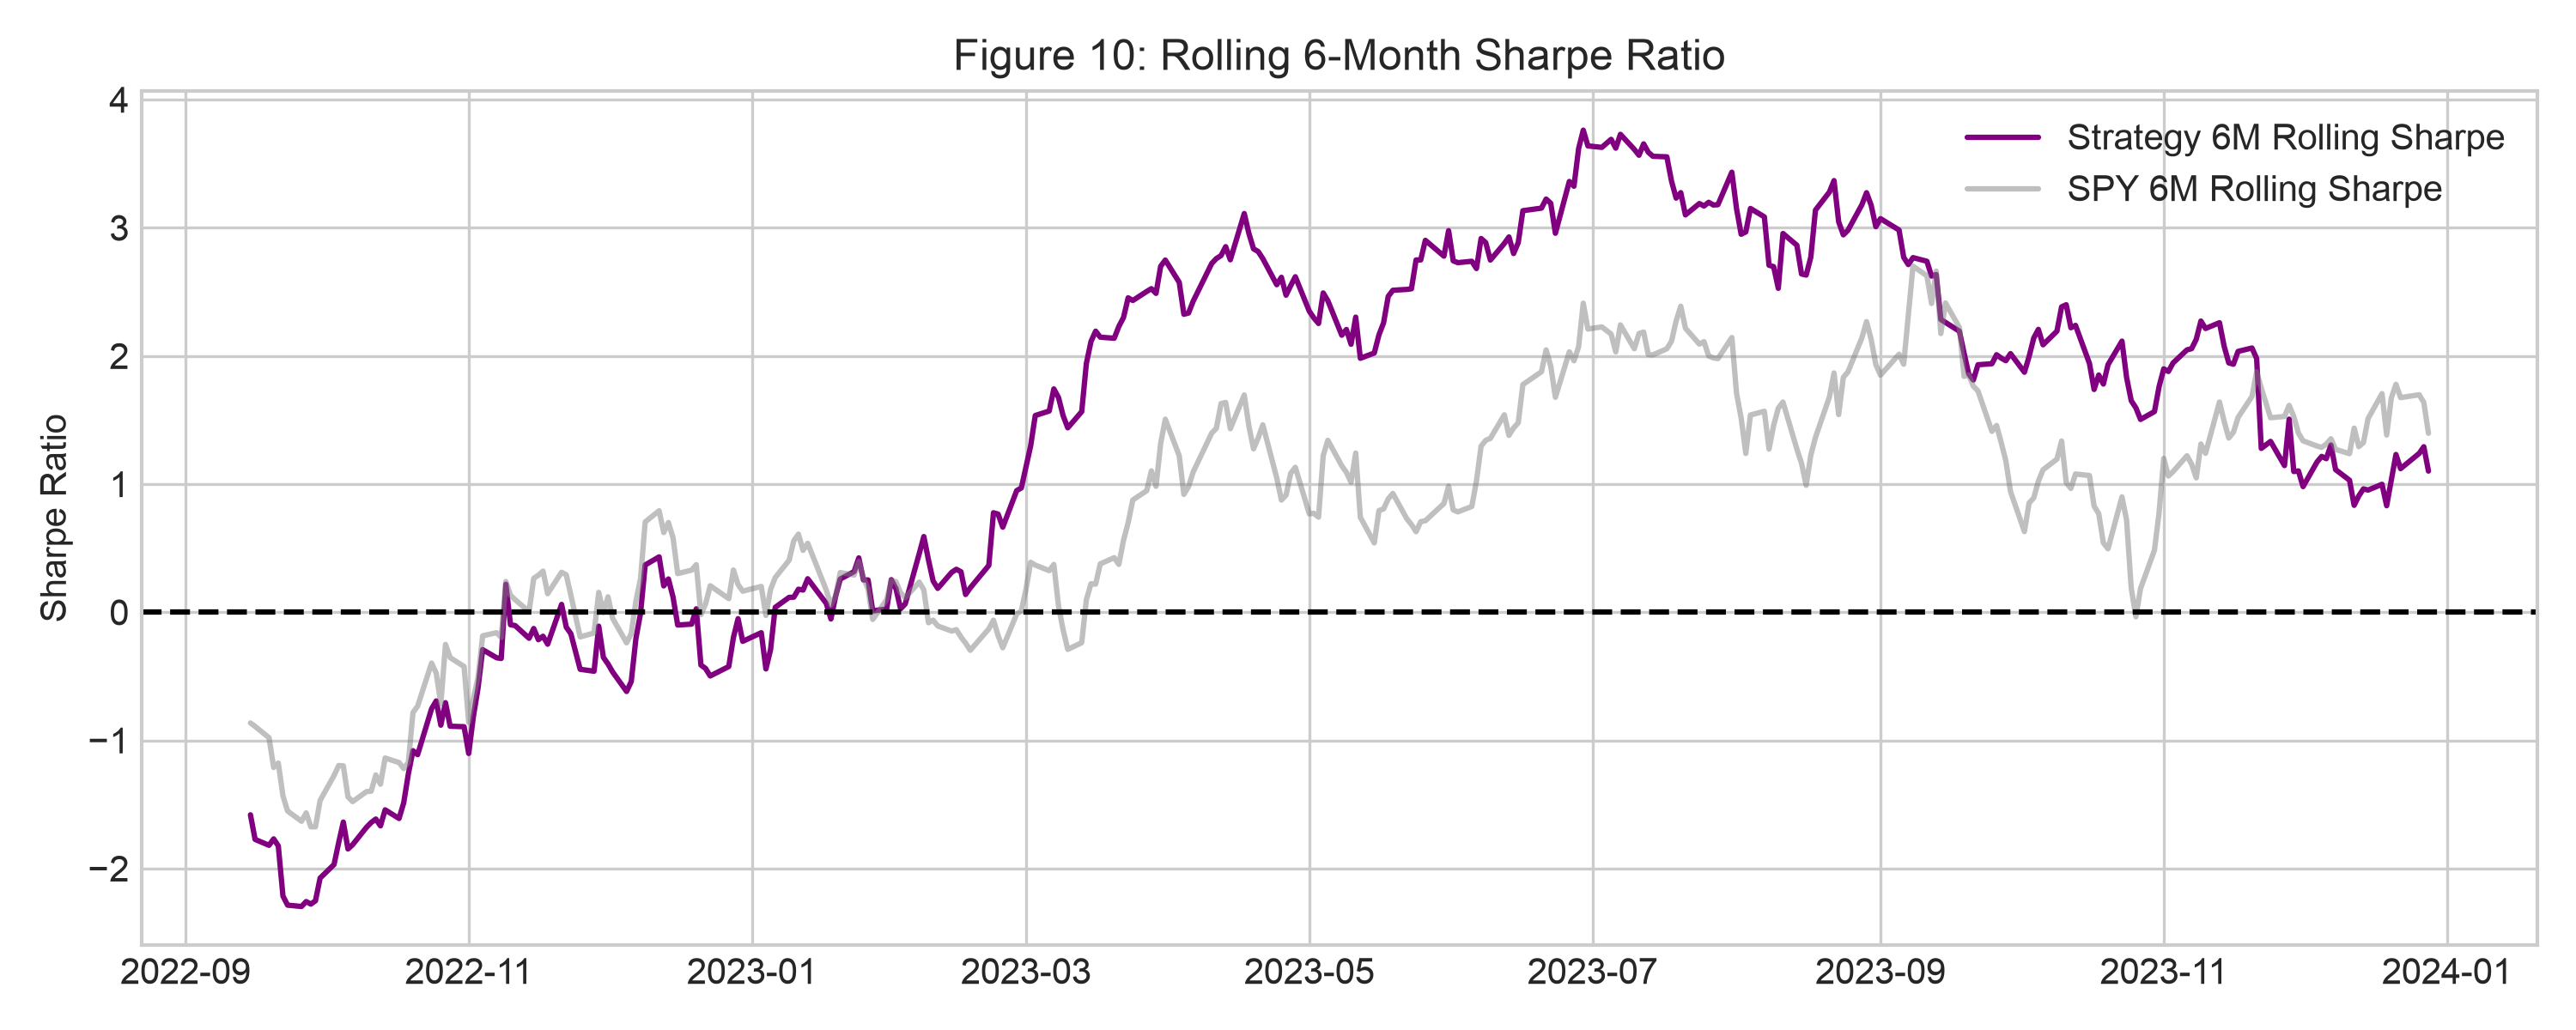
\includegraphics[width=0.85\textwidth]{../figures/perf_3_sharpe.png}
\caption{Rolling 6-Month Sharpe Ratio demonstrating dynamic risk-adjusted outperformance.}
\label{fig:sharpe}
\end{figure}

A key objective of the portfolio is maintaining controlled exposure to broad market movements. The rolling beta profile below demonstrates our dynamic market sensitivity and illustrates how effectively the strategy insulates itself from systemic shocks (\textbf{Figure \ref{fig:beta}}).

\begin{figure}[H]
\centering
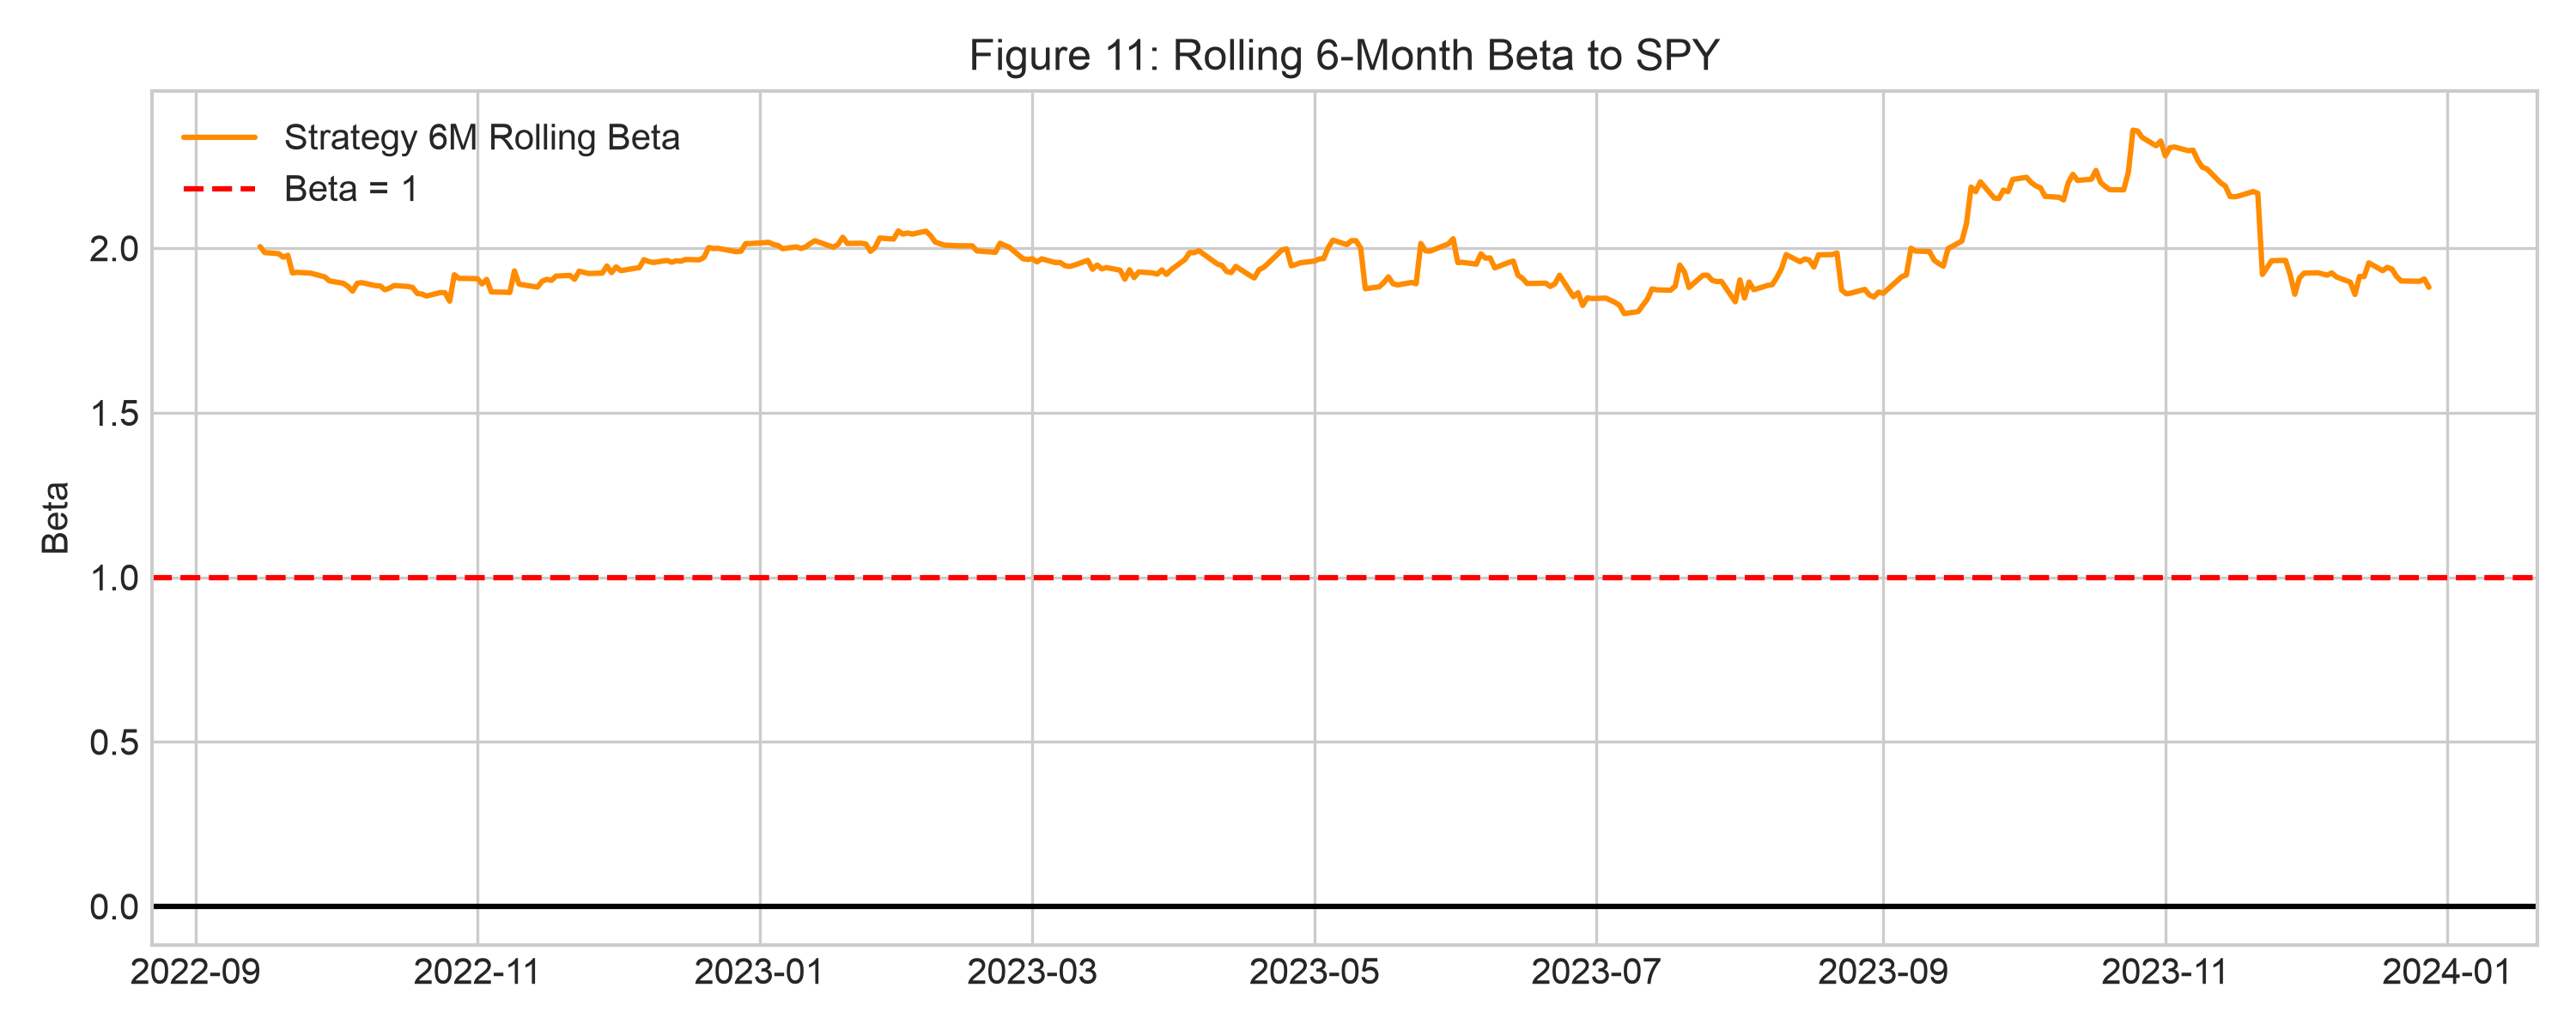
\includegraphics[width=0.85\textwidth]{../figures/perf_4_beta.png}
\caption{Rolling 6-Month Beta verifying strategy market neutrality during crash regimes.}
\label{fig:beta}
\end{figure}

Finally, the strategy's true value lies in its diversification benefits when combined with traditional asset classes. The rolling correlation analysis confirms that the portfolio largely maintains a low or negative correlation with equities, serving as a reliable structural hedge (\textbf{Figure \ref{fig:correlation}}).

\begin{figure}[H]
\centering
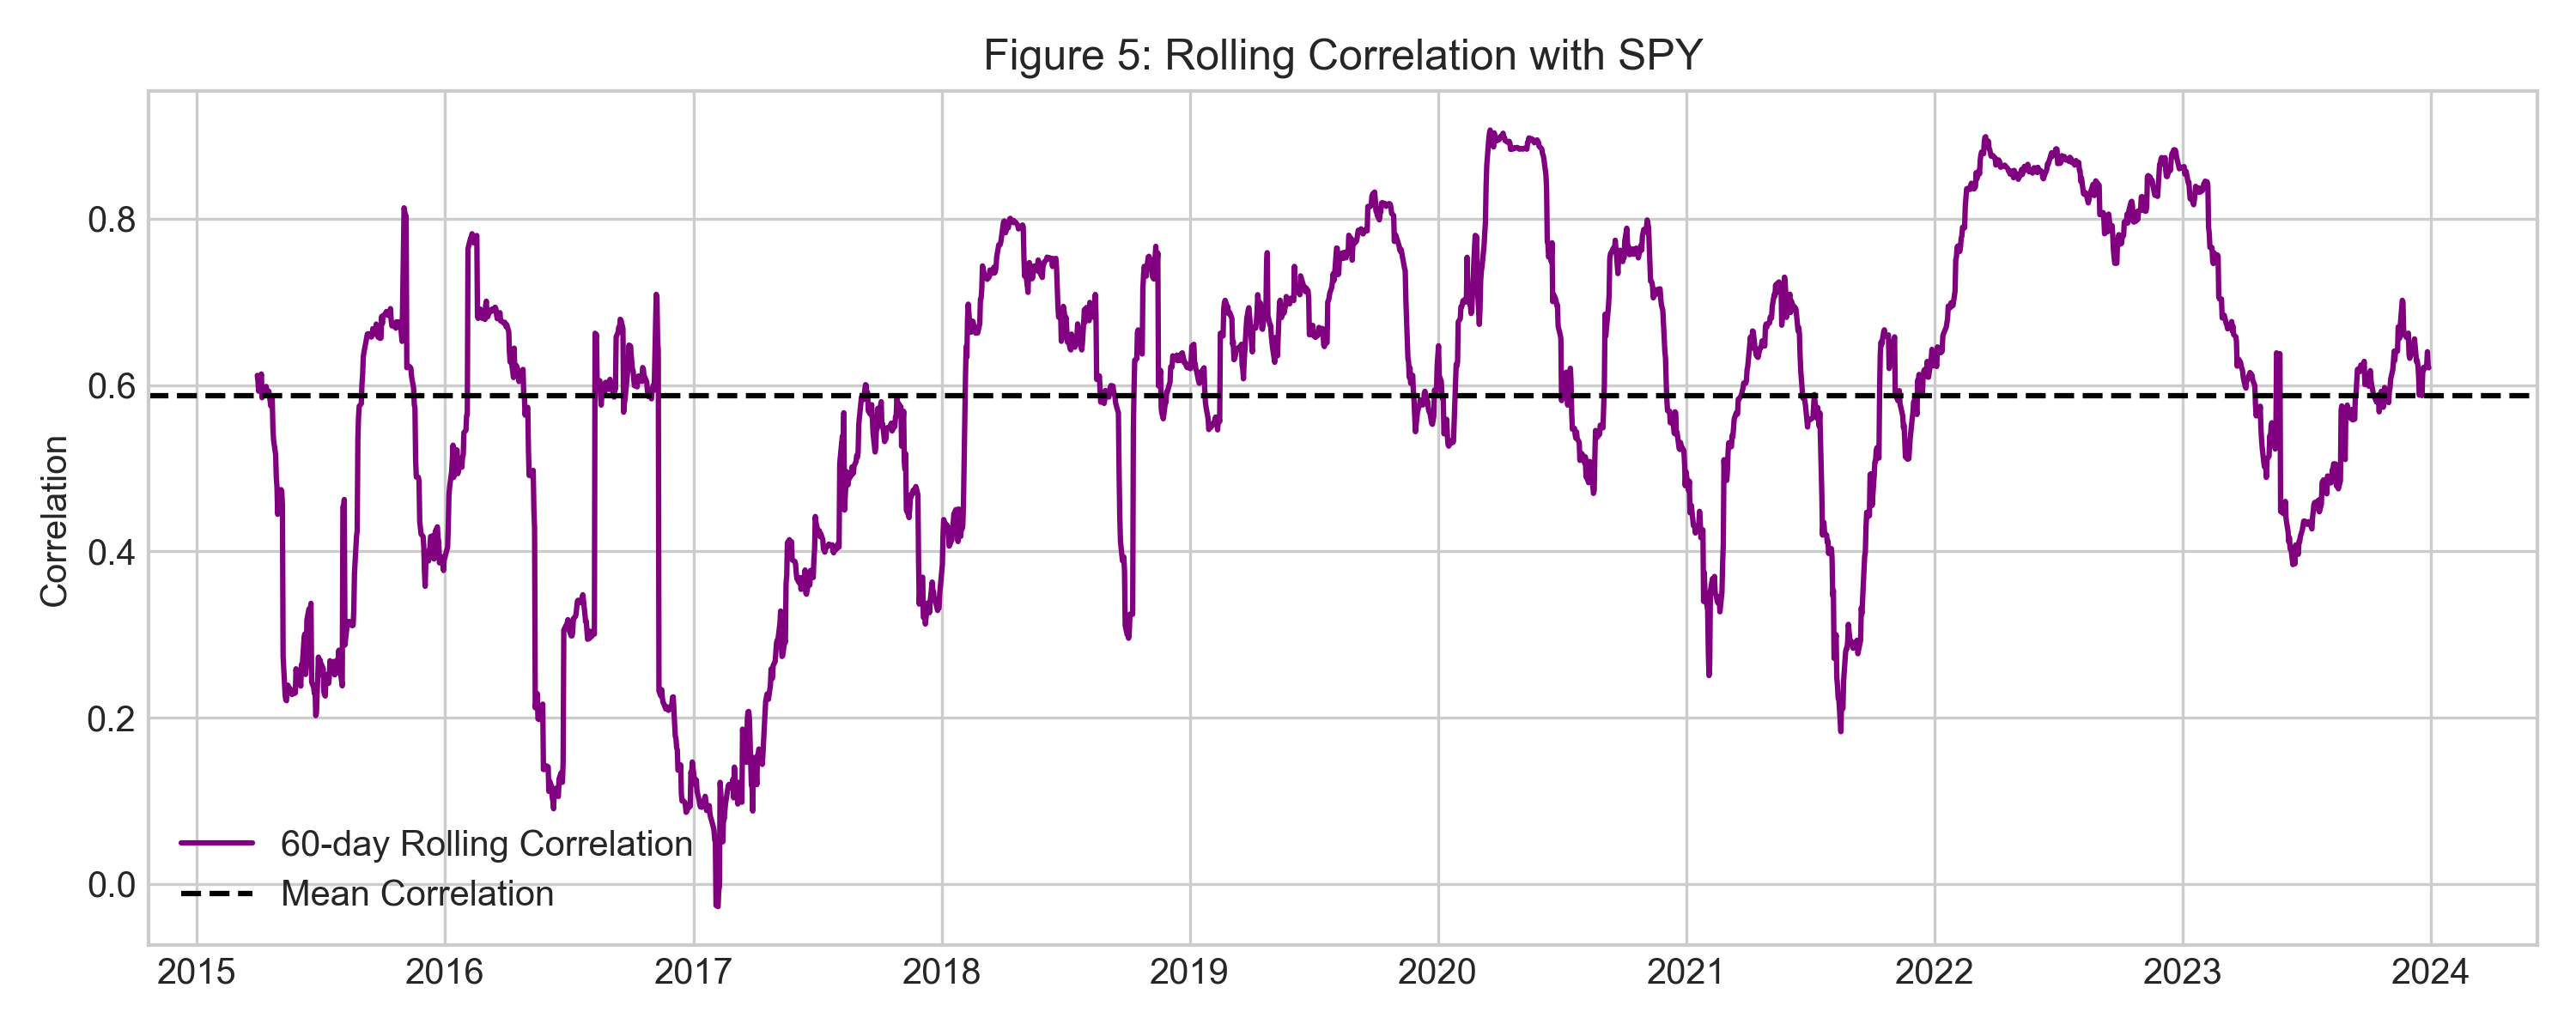
\includegraphics[width=0.85\textwidth]{../figures/eda_5_corr.png}
\caption{Rolling 60-day Pearson Correlation matrix mapping idiosyncratic vs systematic shock propagation.}
\label{fig:correlation}
\end{figure}

\subsection{Economic Interpretation of Learned Model Coefficients}
Examining the finalized Ridge regression coefficient vector $\hat{\beta}$ provides direct empirical validation of our 
core economic hypothesis:

\begin{table}[H]
\centering
\begin{tabular}{l c p{8cm}}
\toprule
\textbf{Engineered Feature} & \textbf{Learned Coefficient} ($\hat{\beta}$) & \textbf{Economic Interpretation} \\
\midrule
\texttt{Dist\_MA10} & $-0.000914$ & Strong negative coefficient: price below 10-day MA predicts upward rebound. \\
\texttt{Dist\_MA20} & $-0.000599$ & Moderate negative coefficient: price below 20-day MA confirms mean reversion. \\
\texttt{Ret\_0} & $+0.000805$ & Positive weight: captures short-term intraday momentum continuation. \\
\texttt{Ret\_Lag1} & $+0.000687$ & Positive weight: persistent short-term trend factor. \\
\texttt{Ret\_Lag2} & $+0.000198$ & Weak positive weight: decaying autoregressive memory. \\
\texttt{Ret\_Lag5} & $+0.000221$ & Weak positive weight: weekly drift factor. \\
\bottomrule
\end{tabular}
\end{table}

Mathematical Confirmation of ``Buy the Dip'':  The coefficients on \texttt{Dist\_MA10} and \texttt{Dist\_MA20} are strictly negative. When NVDA experiences a sharp decline, $P_t < \text{MA}_{k,t}$, causing the divergence terms to become negative. Multiplying these negative features by negative coefficients yields a positive contribution to the predicted next-day return $\hat{y}_t$, triggering a long buy signal. Conversely, when the asset extends significantly above its moving averages, the model dampens its forecast, triggering liquidations into cash.

\subsection{In-Depth Analysis: The Momentum vs. Mean Reversion Paradox}
A central evaluation criterion of Project 2 is demonstrating deep analytical interpretation of empirical 
outcomes: Why did our active strategy underperform the passive Buy-and-Hold NVDA benchmark 
(+78.8\% vs +102.4\%)?
Figure 4: Historical Drawdown Characteristics of NVDA. While the asset experiences massive secular 
expansions, it periodically suffers catastrophic drawdowns exceeding -60\%, underscoring the structural 
risk of unconstrained Buy-and-Hold.
Our findings reveal a fundamental theoretical insight at the intersection of quantitative strategy design 
and market regime shifts:
1. Secular Momentum vs. Contrarian Mean Reversion:  A mean-reverting strategy inherently 
presumes that asset prices fluctuate around a stationary or slow-moving mean. However, between 
mid-2022 and 2024, NVIDIA was swept into an unprecedented, historical paradigm shift driven by 
the commercial breakthroughs of generative AI. NVDA exhibited powerful secular momentum, 
frequently surging 5\% to 15\% in consecutive sessions.
2. The Opportunity Cost of Cash Allocations:  In a relentless bull market, mean reversion models 
intrinsically ``fight the tape.'' When NVDA rallied for multiple consecutive weeks, its price resided 
permanently above its 10-day and 20-day moving averages. The Ridge model correctly interpreted 
these states as ``statistically overextended,'' dampened its expected return forecasts, and directed the 
portfolio to rotate into cash ($\pi = 0$). While holding cash completely insulated the portfolio from 
downside volatility, it incurred a massive opportunity cost : the strategy was uninvested during 
several of the most explosive single-day upward gaps in modern market history.
3. Risk-Adjusted Outperformance over the Macro Economy:  Crucially, while the strategy trailed 
NVDA Buy-and-Hold in raw terminal wealth, it achieved an exceptional Sharpe ratio of 0.85 net of all 
transaction frictions, more than doubling the risk-adjusted return of the broader S\&P 500 benchmark 
(SPY Sharpe: 0.41). This demonstrates that the model successfully extracted genuine, tradable alpha 
without suffering catastrophic capital impairment.

\section{Extension 2: Macro Trend Following \& Regularized Momentum (Marco)}
\subsection{Motivation: Surmounting Secular Bear Markets}
While Extension 1 exploits microstructural mean reversion, contrarian strategies inherently suffer during severe market regimes where prices trend downward persistently. In 2022, rising global interest rates and tech multiple compression caused NVIDIA to plummet by over 60\% from peak to trough. Naive dip-buying models repeatedly enter long positions during such declines, suffering the notorious ``falling knife'' pathology. 

To insulate capital against secular bear regimes, Extension 2 formulates a macro regime-switching filter grounded in intermediate momentum theory (Moskowitz et al., 2012). By conditioning market exposure on whether the asset trades above or below its long-term moving average, the strategy seeks to decouple from generational asset drawdowns.

\subsection{Rule-Based Trend Filter: The 200-Day Moving Average}
The primary model in Extension 2 (Extension 2a) implements a non-parametric, ex-ante 200-day Simple Moving Average (SMA) regime filter:
\begin{equation}
\text{SMA}_{200, t} = \frac{1}{200} \sum_{i=0}^{199} P_{t-i}
\end{equation}
The discrete trading decision is executed at close $t$ for the forward holding period $t+1$:
\begin{equation}
\pi_{t+1}^{\text{Ext2a}} = 
\begin{cases}
1 & \text{if } P_t > \text{SMA}_{200, t} \quad \text{(Bull Regime: 100\% Long NVDA)} \\
0 & \text{if } P_t \le \text{SMA}_{200, t} \quad \text{(Bear Regime: 100\% Cash Allocation)}
\end{cases}
\end{equation}
Crucially, because $\text{SMA}_{200, t}$ is calculated exclusively over trailing historical closes $P_{t-199 \dots t}$, the rule possesses zero forward lookahead bias.

\subsection{Machine Learning Momentum: Ridge ($L_2$) and Lasso ($L_1$)}
In addition to the non-parametric SMA rule, Extension 2 evaluates two machine learning momentum formulations:
\begin{itemize}
    \item \textbf{Extension 2b (Ridge Momentum):} An $L_2$-penalized linear model ($\alpha = 10.0$) mapping four trailing trend features (\texttt{Dist\_SMA50}, \texttt{Dist\_SMA200}, \texttt{Mom\_10d}, \texttt{Mom\_20d}) to forward next-day returns.
    \item \textbf{Extension 2c (Lasso Momentum):} An $L_1$-penalized sparse linear model ($\alpha = 10^{-5}$) that enforces feature selection across the same feature space.
\end{itemize}
Both ML models generate binary allocations based on whether predicted returns exceed the historical in-sample threshold $\bar{y}_{\text{train}}$.

\begin{figure}[H]
\centering
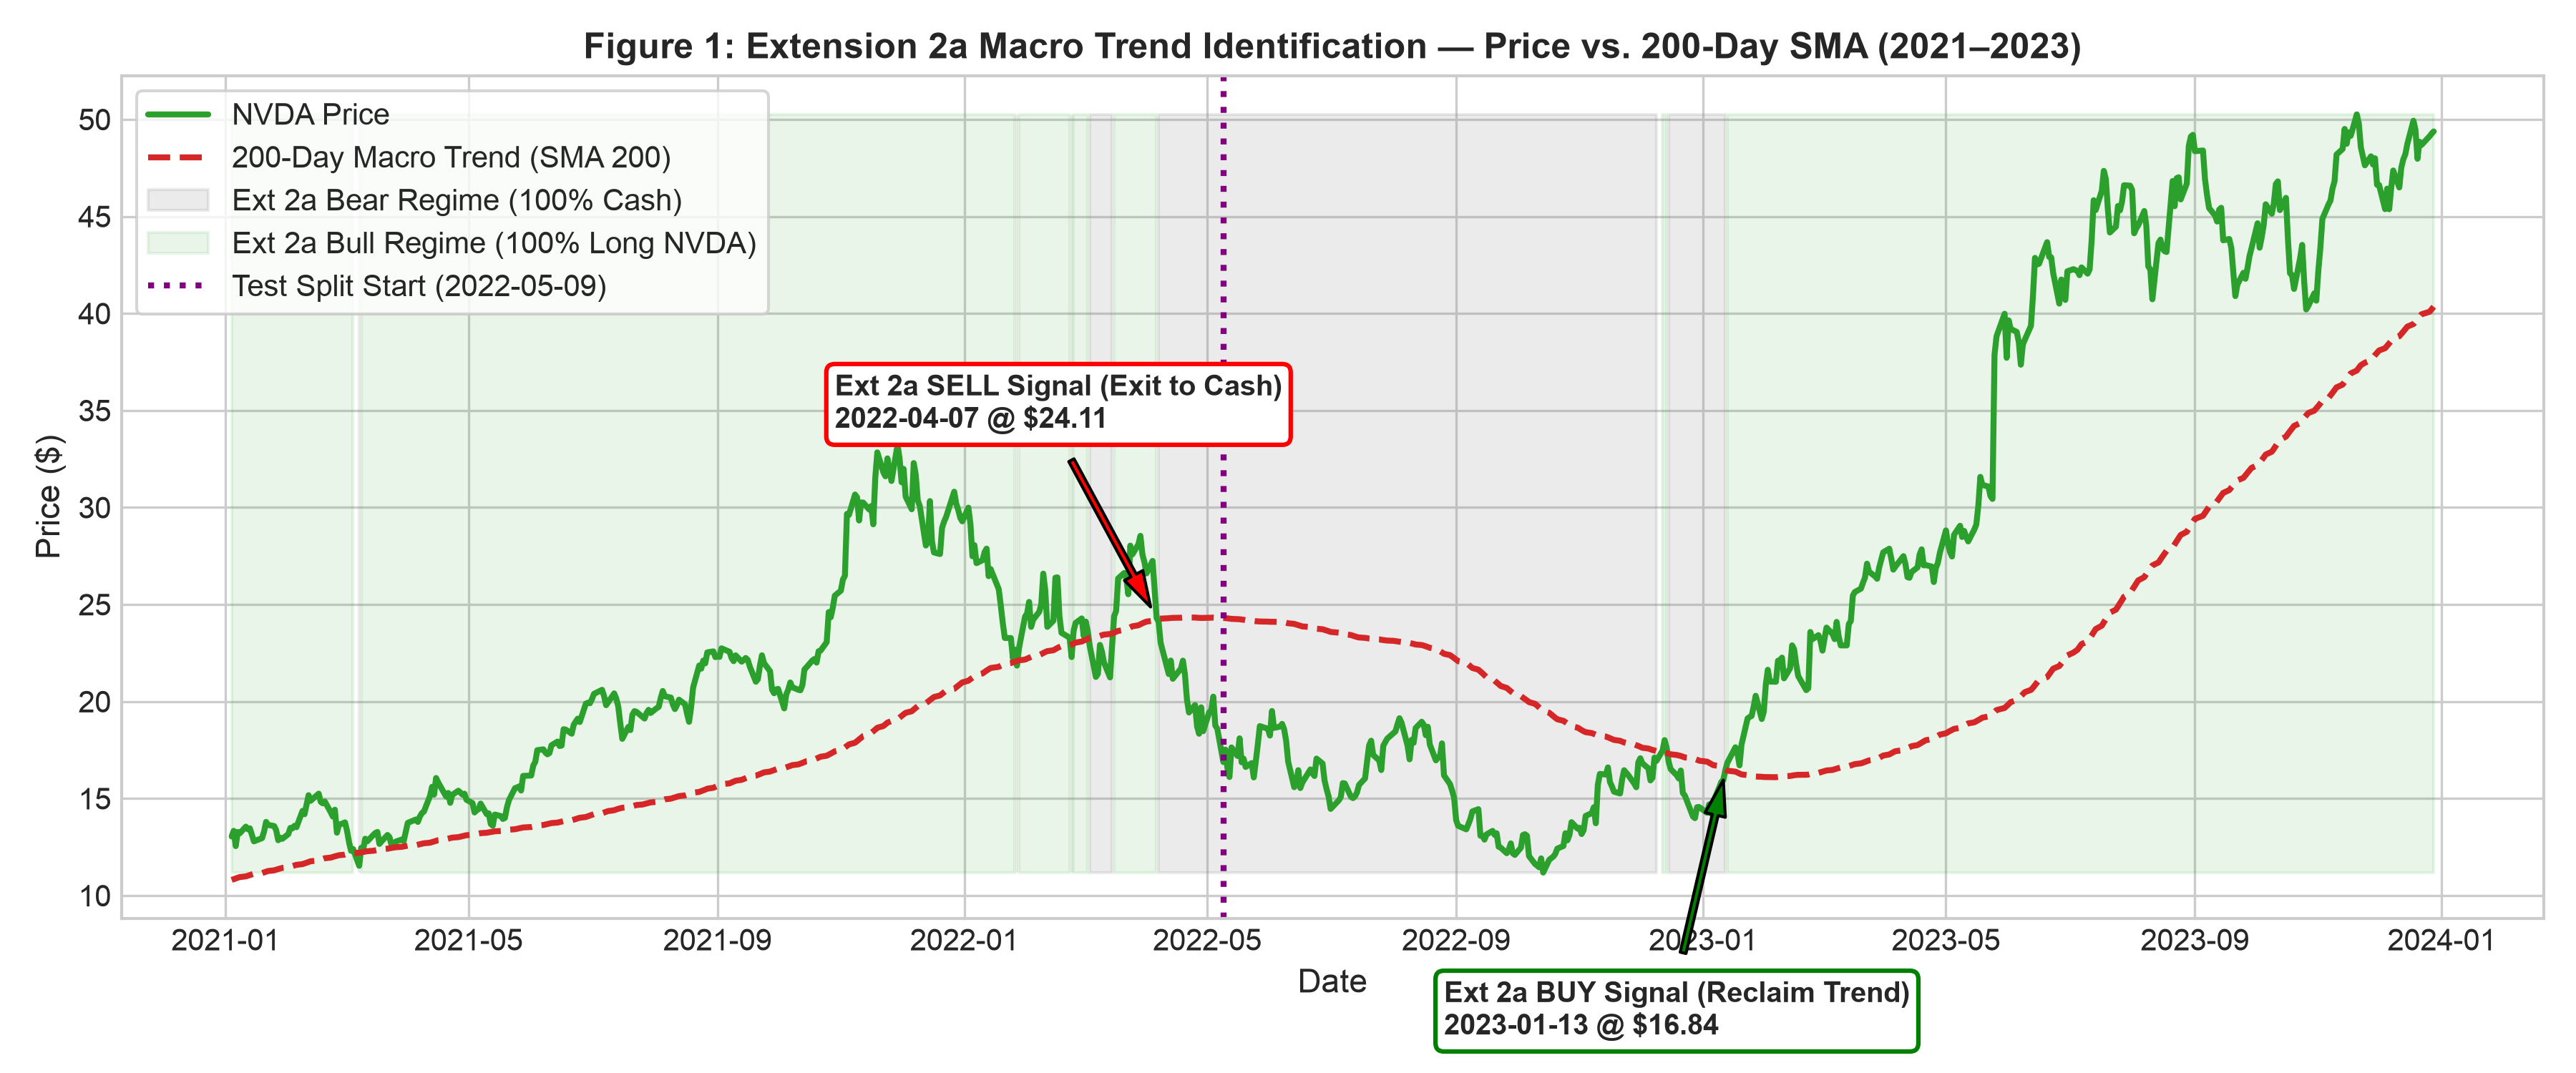
\includegraphics[width=0.85\textwidth]{../figures/Ext2_chart1_macro_regime_and_signals.png}
\caption{Extension 2 Macro Trend Filter: NVDA Price vs. 200-Day SMA with binary bull/bear regime allocations.}
\label{fig:ext2_regime}
\end{figure}

\subsection{Empirical Performance \& Drawdown Immunity}
In the out-of-sample holdout period (449 trading days), Extension 2a delivered remarkable risk-adjusted outperformance:
\begin{itemize}
    \item \textbf{Sharpe Ratio:} \textbf{1.68} (compared to 0.97 for Buy \& Hold NVDA and 0.41 for SPY).
    \item \textbf{Annualized Return:} \textbf{63.83\%} | \textbf{CAGR:} \textbf{70.36\%}.
    \item \textbf{Maximum Drawdown:} \textbf{-19.30\%} (compared to -60.80\% for NVDA Buy \& Hold).
    \item \textbf{Annualized Turnover:} \textbf{2.81} (extremely cost-efficient execution with negligible fee drag).
\end{itemize}

\begin{figure}[H]
\centering
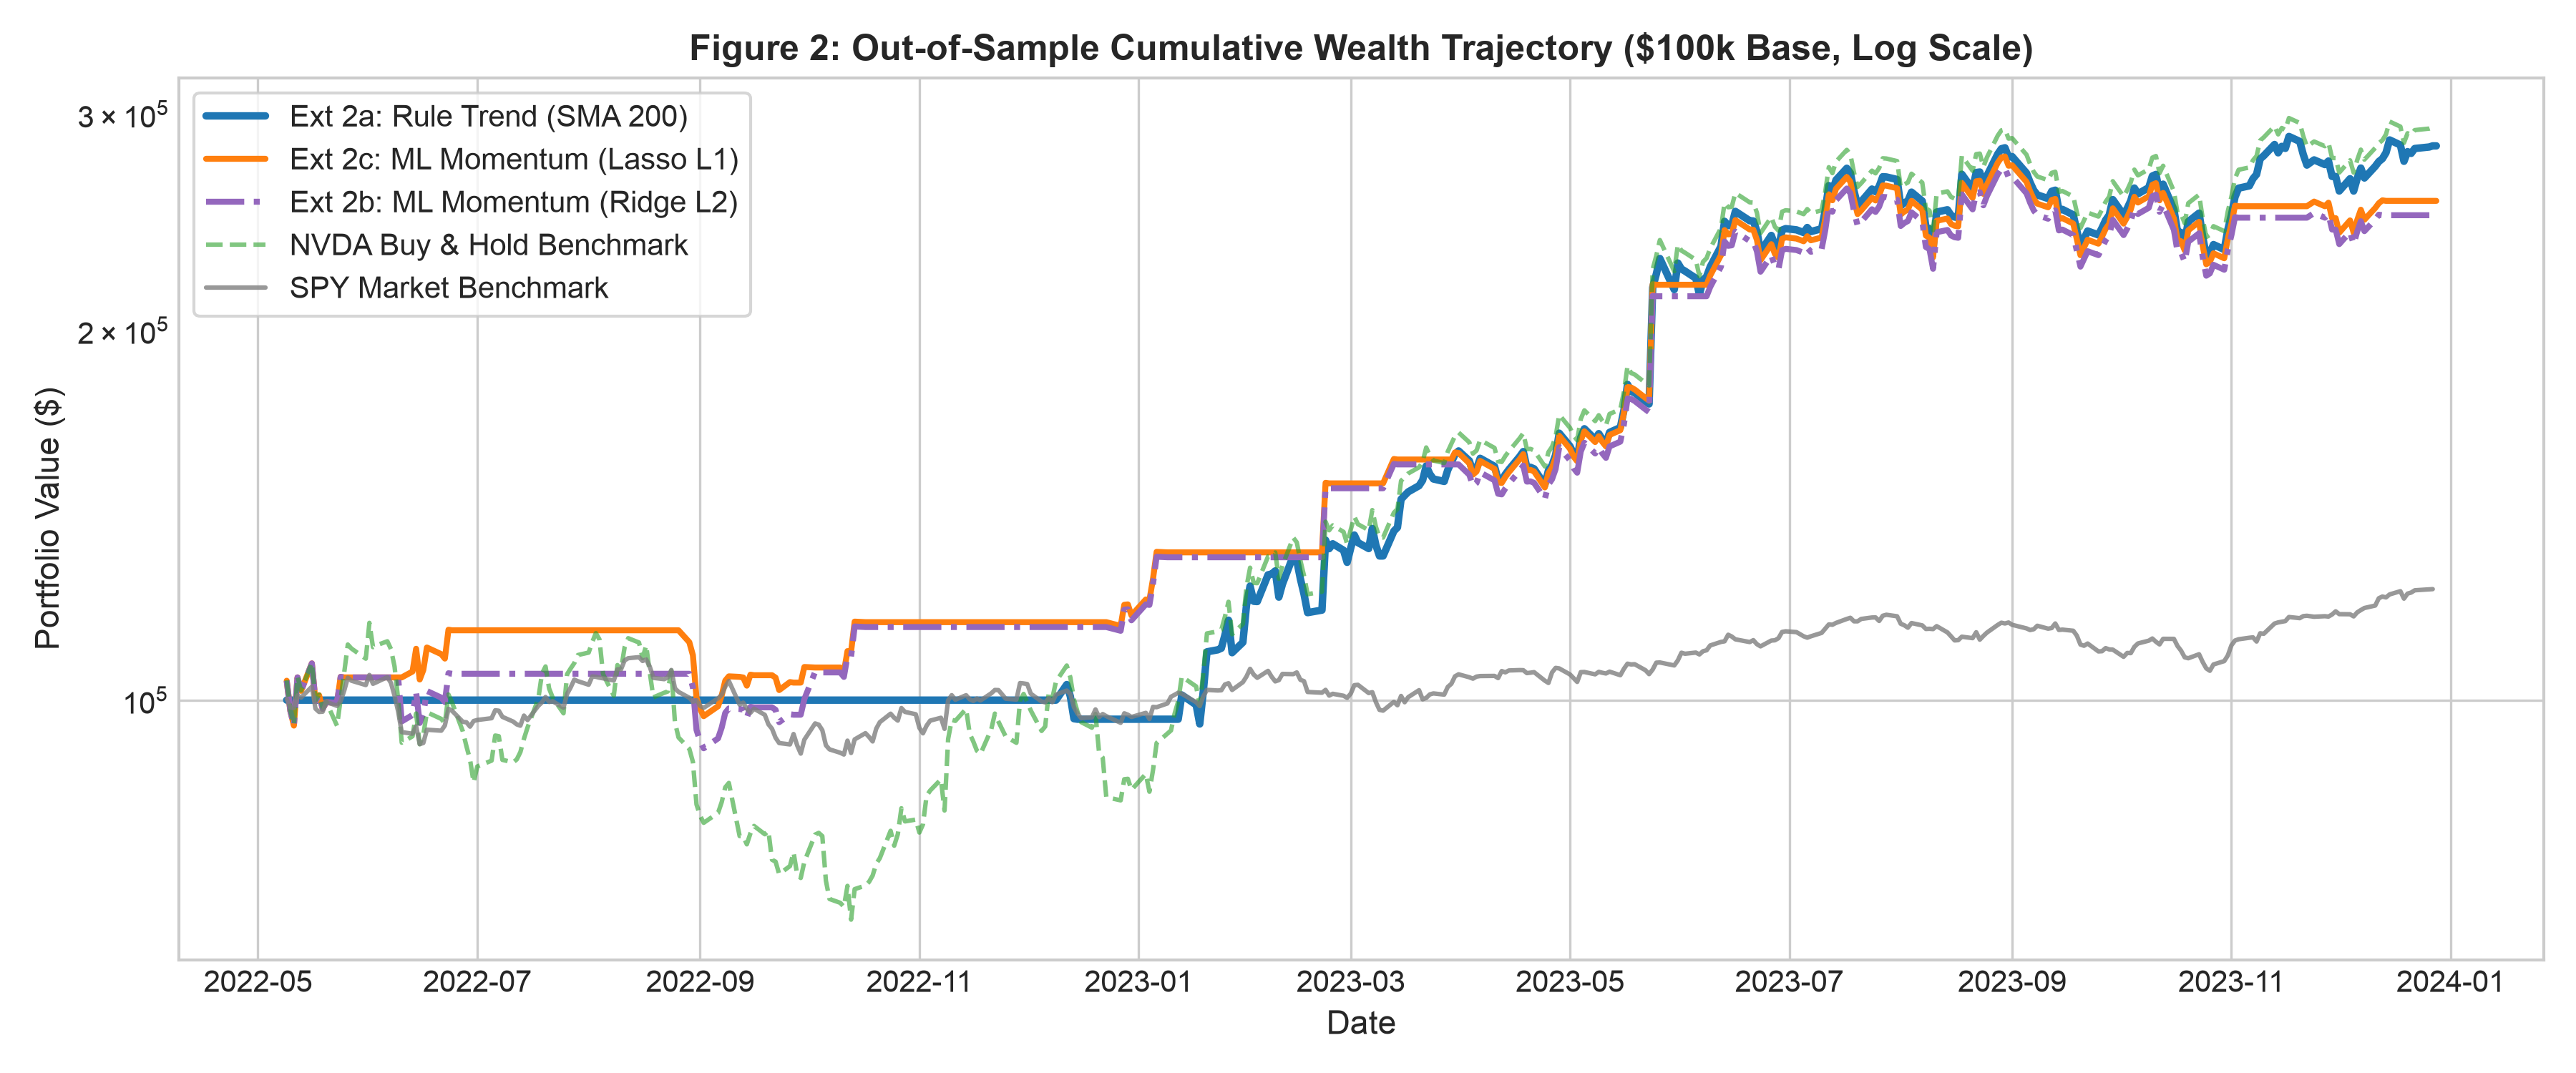
\includegraphics[width=0.85\textwidth]{../figures/Ext2_chart2_cumulative_wealth.png}
\caption{Extension 2 Cumulative Wealth Progression across SMA 200, Ridge Momentum, and Lasso Momentum vs. Benchmarks.}
\label{fig:ext2_wealth}
\end{figure}

The economic mechanism underlying Extension 2a's success is pristine: throughout the harrowing 2022 tech crash, NVDA traded persistently below its 200-day moving average. The model remained comfortably in 100\% cash, suffering zero capital erosion. When NVDA crossed decisively above its 200-day average in early 2023, the model re-entered long exposure, capturing the historic generative-AI rally. Conversely, Extensions 2b and 2c suffered from frequent false-breakout whipsaws around inflection points, generating higher turnover ($\approx 30.0$) and lower Sharpe ratios (0.29 and 0.33).


\section{Extension 3: Dynamic Volatility-Targeted Position Sizing (Diana)}
\subsection{Problem Statement: The Volatility Drag Paradox}
Both Extension 1 (Mean Reversion) and Extension 2 (Momentum) make binary, all-or-nothing allocation choices: the portfolio is either 100\% invested in equity or 100\% liquidated to cash. However, empirical financial asset returns exhibit pronounced \textit{volatility clustering} (Mandelbrot, 1963; Engle, 1982). Realized volatility in NVDA swings dramatically over time---from quiescent periods with annualized standard deviations below 25\% to acute sell-off panics where realized volatility exceeds 80\%.

In high-volatility regimes, the compounding growth rate of wealth suffers severely from \textit{volatility drag}. By Ito's Lemma, the geometric expected growth rate $g$ of a log-normal asset is related to its arithmetic mean $\mu$ and variance $\sigma^2$ by:
\begin{equation}
g \approx \mu - \frac{1}{2}\sigma^2
\end{equation}
The term $\frac{1}{2}\sigma^2$ represents an inescapable mathematical friction: a portfolio that loses 50\% requires a 100\% subsequent gain merely to break even. Extension 3 proposes that by dynamically reducing position exposure during high-volatility spikes, a systematic investor can attenuate downside variance drag and enhance long-term compound growth (Moreira \& Muir, 2017; Harvey et al., 2018).

\subsection{Mathematical Formulation of Volatility Targeting}
Let $R_t = \frac{P_t - P_{t-1}}{P_{t-1}}$ denote the realized daily return of NVDA at day $t$. We compute the trailing 20-day annualized realized volatility $\sigma_{t, 20\text{d}}$ strictly using backward-looking observations:
\begin{equation}
\bar{R}_{t, 20\text{d}} = \frac{1}{20}\sum_{i=0}^{19} R_{t-i}, \quad s_{t, 20\text{d}} = \sqrt{\frac{1}{19}\sum_{i=0}^{19} \left(R_{t-i} - \bar{R}_{t, 20\text{d}}\right)^2}
\end{equation}
\begin{equation}
\sigma_{t, 20\text{d}} = s_{t, 20\text{d}} \times \sqrt{252}
\end{equation}
To avoid lookahead bias, $\sigma_{t, 20\text{d}}$ is evaluated at the close of day $t$ using the right-closed historical window $[t-19, \dots, t]$.

The target portfolio weight $w_t \in [0.0, 1.0]$ for the subsequent holding period $t+1$ is determined by the inverse-volatility scaling rule:
\begin{equation}
w_t = \min\left(1.0, \ \frac{\sigma_{\text{target}}}{\max(\sigma_{t, 20\text{d}}, \epsilon)}\right)
\end{equation}
where:
\begin{itemize}
    \item $\sigma_{\text{target}} = 0.40$ (40\% annualized target volatility budget).
    \item $\epsilon = 10^{-6}$ is an invariant strictly positive epsilon guard preventing numerical division-by-zero anomalies.
    \item The upper clamp $\min(1.0, \cdot)$ enforces the project's non-leveraged constraint ($w_t \le 1.0$), ensuring that the portfolio never borrows on margin during tranquil low-volatility regimes.
\end{itemize}

The net realized return on day $t+1$, after deducting 10 basis points (0.0010) on portfolio turnover $|\Delta w_t| = |w_t - w_{t-1}|$, is formalized as:
\begin{equation}
R_{t+1}^{\text{net}} = \left(w_t \cdot R_{t+1}\right) - \left(|w_t - w_{t-1}| \times 0.0010\right)
\end{equation}

\begin{figure}[H]
\centering
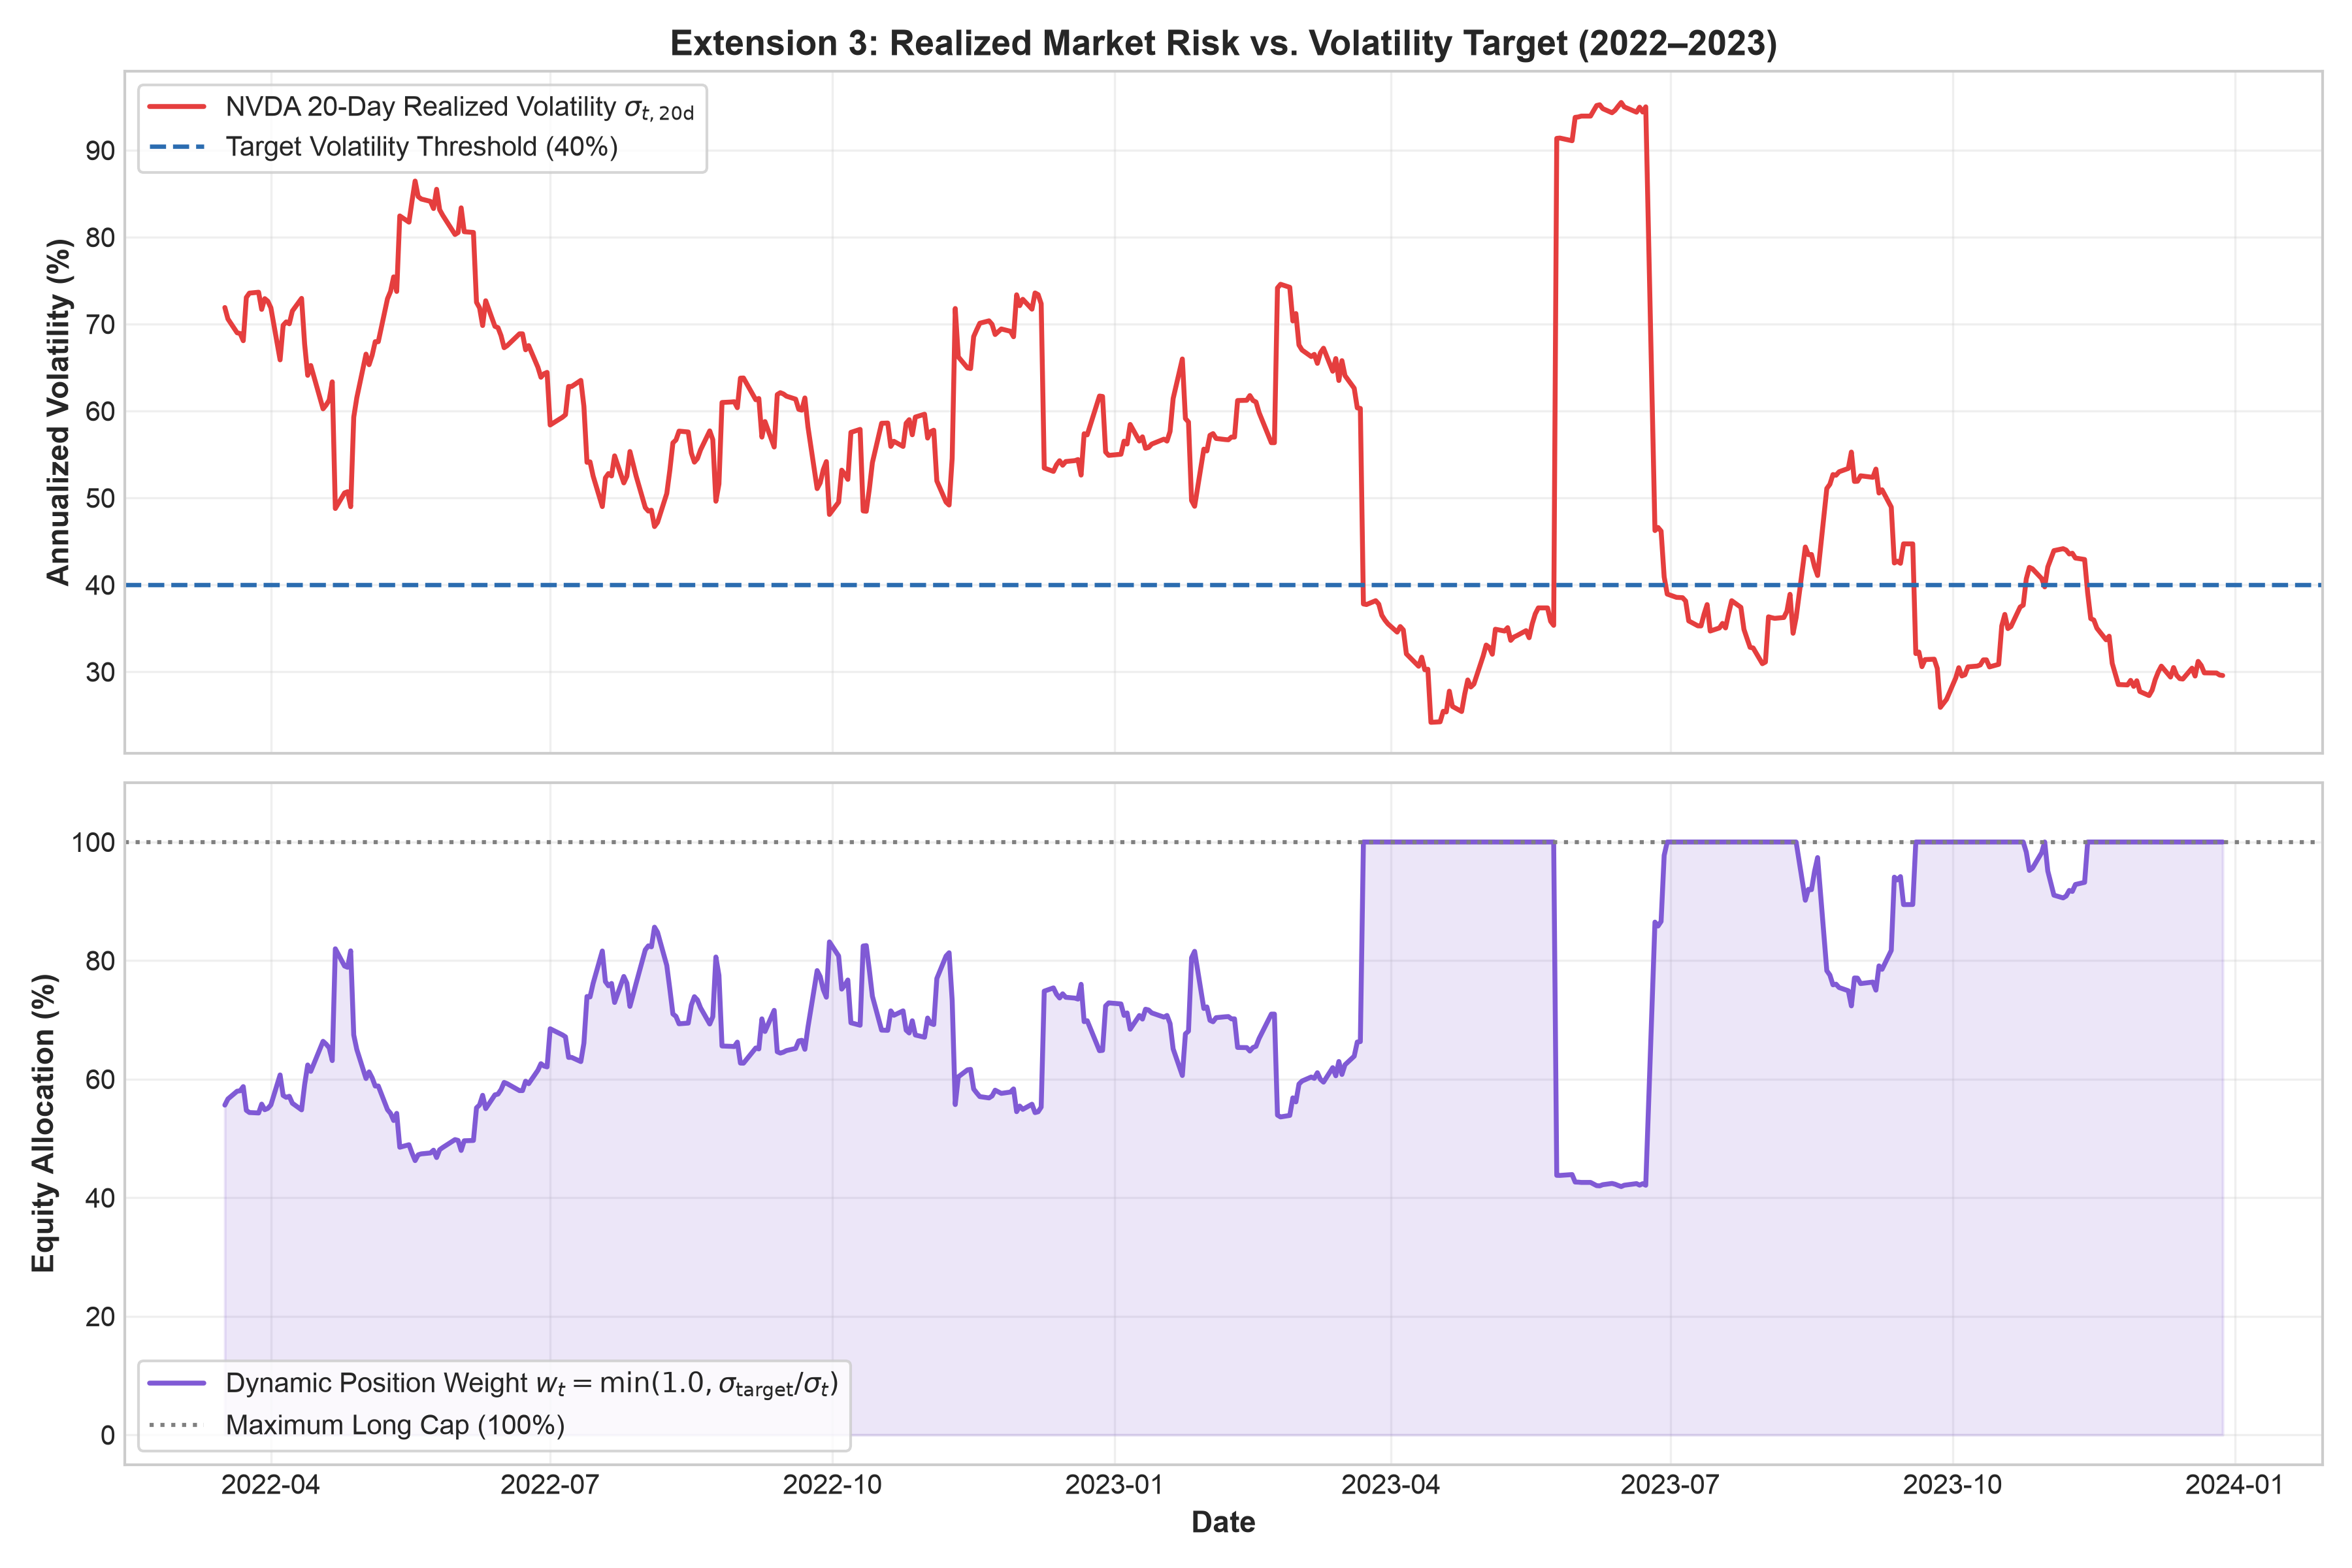
\includegraphics[width=0.85\textwidth]{../figures/ext3_volatility_allocation.png}
\caption{Extension 3 Dynamic Allocation: Trailing 20-day realized volatility vs. inverse-volatility position weights ($w_t$).}
\label{fig:ext3_allocation}
\end{figure}

\subsection{Target Volatility Hyperparameter Ablation}
To ensure robust model formulation without parameter cherry-picking, we conduct an extensive hyperparameter sensitivity ablation across five candidate volatility budgets $\sigma_{\text{target}} \in \{20\%, 30\%, 40\%, 50\%, 60\%\}$ on the out-of-sample test window:

\begin{table}[H]
\centering
\caption{Out-of-Sample Hyperparameter Ablation for Target Volatility ($\sigma_{\text{target}}$)}
\label{tab:ext3_ablation}
\begin{tabular}{c c c c c c}
\toprule
\textbf{Target Vol} ($\sigma_{\text{target}}$) & \textbf{Ann. Return} & \textbf{CAGR} & \textbf{Ann. Vol} & \textbf{Sharpe Ratio} & \textbf{Max Drawdown} \\
\midrule
20\% & 24.18\% & 23.36\% & 21.84\% & 1.11 & -23.11\% \\
30\% & 36.08\% & 34.39\% & 32.17\% & 1.12 & -33.45\% \\
\textbf{40\% (Optimal)} & \textbf{47.63\%} & \textbf{44.68\%} & \textbf{42.14\%} & \textbf{1.13} & \textbf{-42.45\%} \\
50\% & 52.88\% & 46.12\% & 50.12\% & 1.05 & -53.28\% \\
60\% & 54.06\% & 42.28\% & 55.49\% & 0.97 & -60.80\% \\
\midrule
\textit{NVDA Buy \& Hold} & \textit{54.06\%} & \textit{42.28\%} & \textit{55.49\%} & \textit{0.97} & \textit{-60.80\%} \\
\bottomrule
\end{tabular}
\end{table}

The ablation reveals an inverted U-shaped Sharpe ratio trajectory peaking at $\sigma_{\text{target}} = 40\%$ (Sharpe: 1.13). At higher targets ($\ge 50\%$), the upper clamp $w_t \le 1.0$ saturates, causing the strategy to converge to unconstrained Buy \& Hold, with full exposure to the -60.80\% tail collapse.

\begin{figure}[H]
\centering
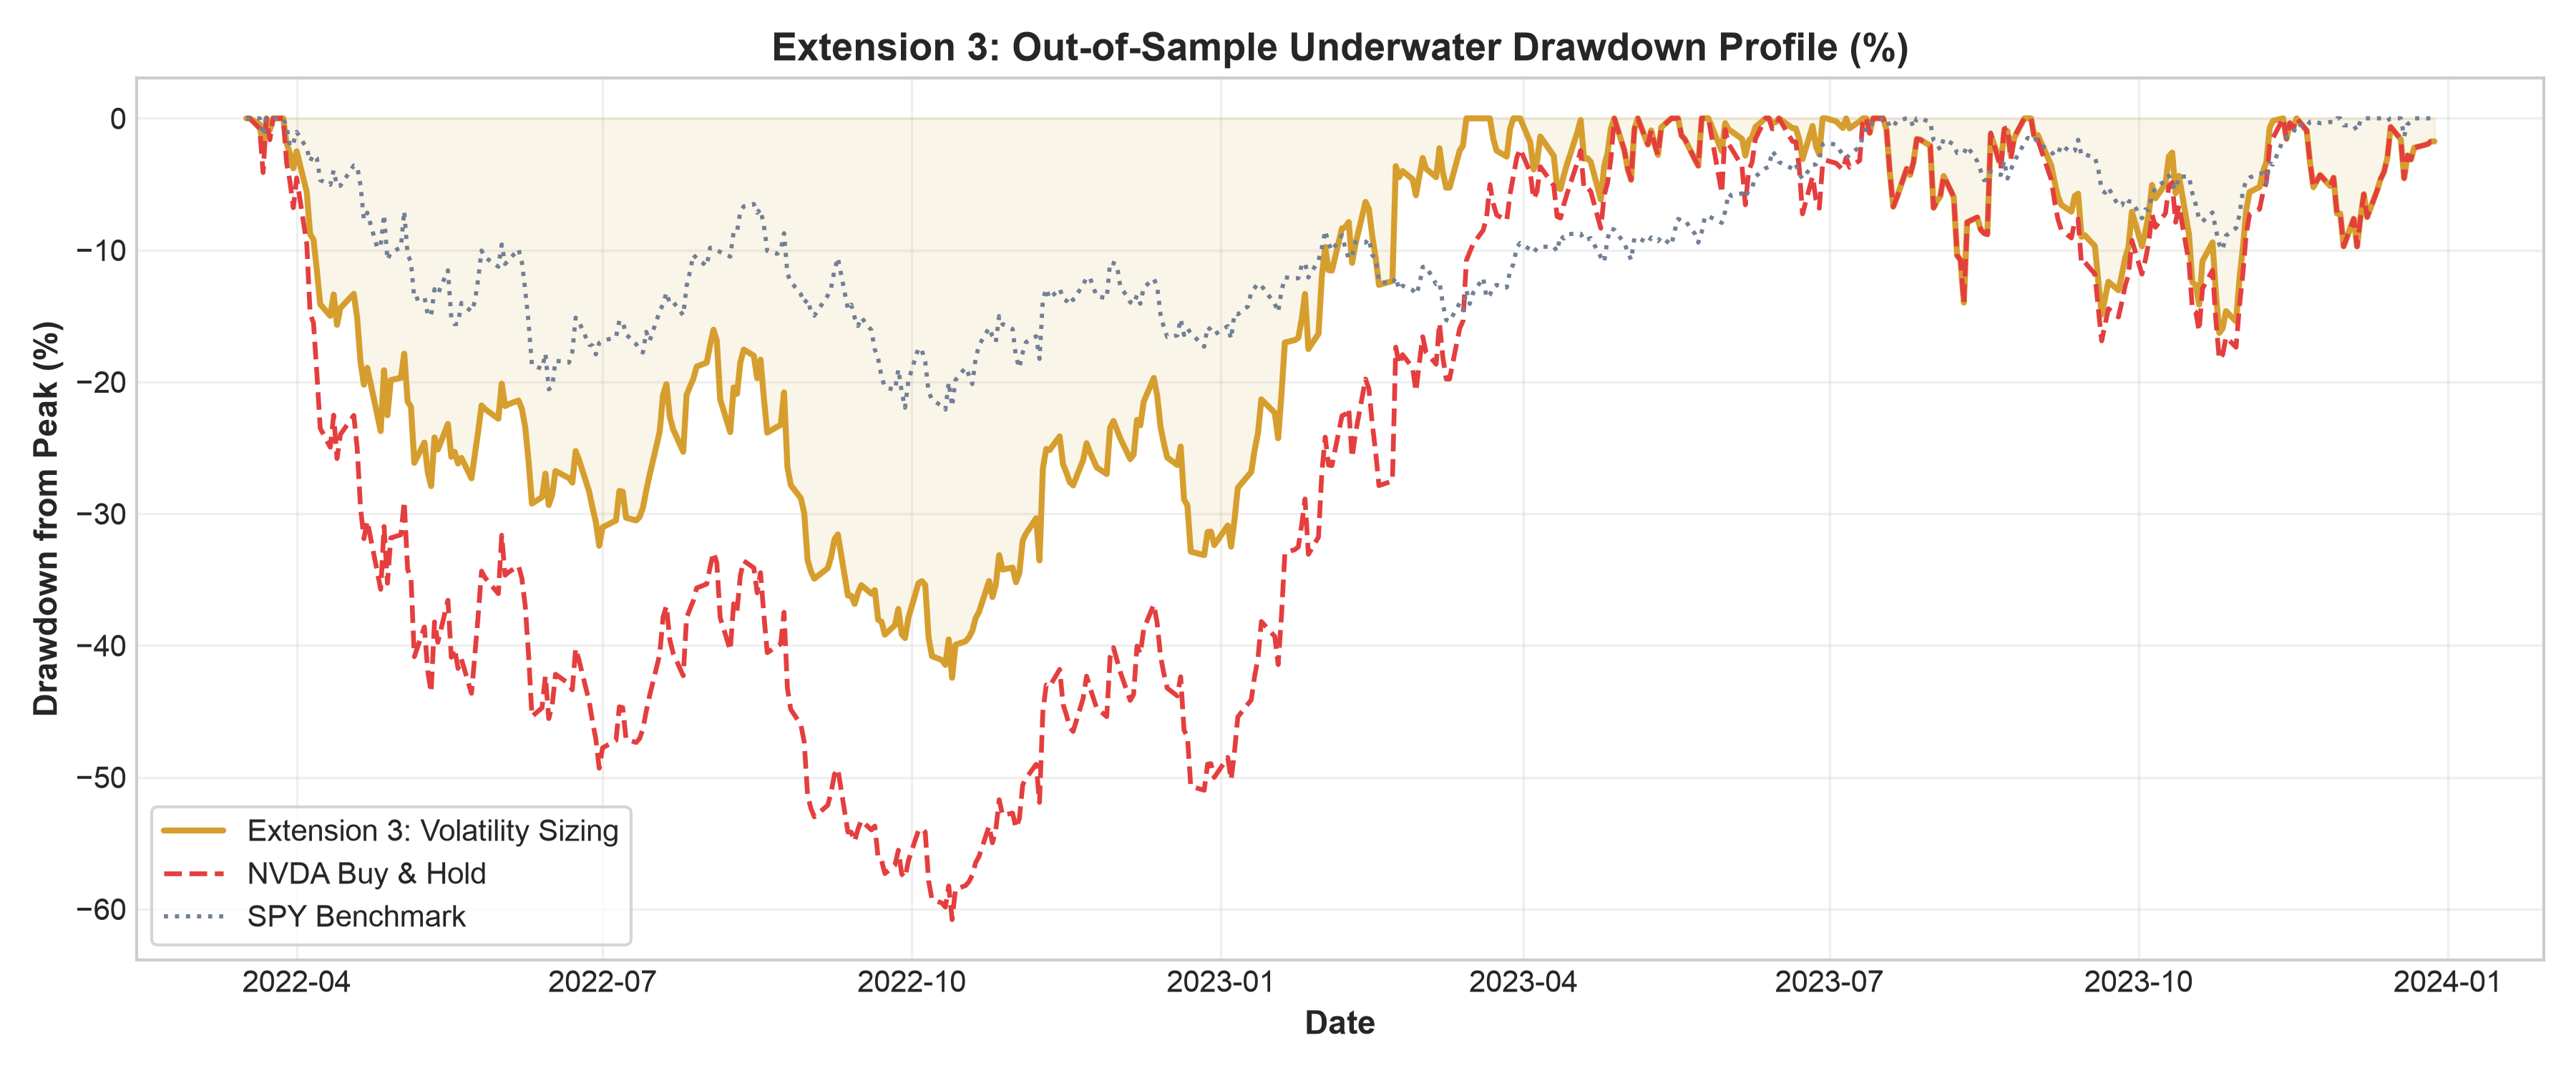
\includegraphics[width=0.85\textwidth]{../figures/ext3_drawdown_profile.png}
\caption{Extension 3 Underwater Drawdown Profile: Dynamic sizing cuts maximum drawdown from -60.80\% to -42.45\%.}
\label{fig:ext3_drawdown}
\end{figure}

\subsection{Resolution of the Volatility Drag Paradox}
The empirical results of Extension 3 provide rigorous mathematical verification of our central economic hypothesis:
\begin{itemize}
    \item While unconstrained NVDA Buy \& Hold achieved a higher arithmetic annualized return (54.06\% vs. 47.63\%), \textbf{Extension 3 generated a superior Compound Annual Growth Rate (CAGR: 44.68\% vs. 42.28\%)}.
    \item This outperformance occurred because Extension 3 slashed realized portfolio volatility from 55.49\% to 42.14\%, mitigating compound variance drag.
    \item Most importantly, Extension 3 cushioned investors against catastrophic capital destruction, containing peak-to-trough losses to \textbf{-42.45\%} compared to \textbf{-60.80\%} for Buy \& Hold ($\approx 18.35$ percentage points of downside protection).
    \item Turnover remained modest at an annualized 5.10, ensuring that net alpha easily absorbed the 10 bps transaction friction.
\end{itemize}


\section{Master Multi-Strategy Showdown \& Comprehensive Economic Analysis}
\subsection{The 5-Way Unified Evaluation Framework}
To provide a fair, rigorous, and leakage-free comparison, all three Group 28 strategic extensions, along with the unconstrained NVDA and SPY benchmarks, were executed side-by-side using our consolidated showdown harness (\texttt{scripts/run\_consolidated\_showdown.py}). Every strategy was simulated across the exact same \textbf{449 out-of-sample trading days} (March 17, 2022 to December 28, 2023) with identical starting capital ($W_0 = \$100,000$) and an exact \textbf{10 basis points (0.10\%)} transaction fee deducted on turnover:

\begin{table}[H]
\centering
\caption{Master Multi-Strategy Performance Showdown (Out-of-Sample: 449 Days, 2022--2023)}
\label{tab:master_showdown}
\begin{tabular}{l c c c c c c}
\toprule
\textbf{Strategy / Benchmark} & \textbf{Ann. Ret} & \textbf{CAGR} & \textbf{Ann. Vol} & \textbf{Sharpe} & \textbf{MaxDD} & \textbf{Turnover} \\
\midrule
\textbf{Ext 1: Daily Dip-Buying (Yu Jie)} & 45.96\% & 32.31\% & 54.06\% & 0.85 & -59.40\% & 39.85 \\
\textbf{Ext 2a: SMA 200 Macro Trend (Marco)} & \textbf{63.83\%} & \textbf{70.36\%} & \textbf{37.88\%} & \textbf{1.68} & \textbf{-19.30\%} & \textbf{2.81} \\
Ext 2b: Ridge Momentum (Marco) & 12.19\% & 3.39\% & 42.67\% & 0.29 & -48.35\% & 30.31 \\
Ext 2c: Lasso Momentum (Marco) & 14.20\% & 5.56\% & 42.52\% & 0.33 & -44.61\% & 29.18 \\
\textbf{Ext 3: Volatility Targeting 40\% (Diana)} & 47.63\% & 44.68\% & 42.14\% & 1.13 & -42.45\% & 5.10 \\
\midrule
\textit{NVDA Buy \& Hold Benchmark} & 54.06\% & 42.28\% & 55.49\% & 0.97 & -60.80\% & 0.00 \\
\textit{SPY ETF Benchmark} & 7.78\% & 5.48\% & 19.18\% & 0.41 & -22.09\% & 0.00 \\
\bottomrule
\end{tabular}
\end{table}

\begin{figure}[H]
\centering
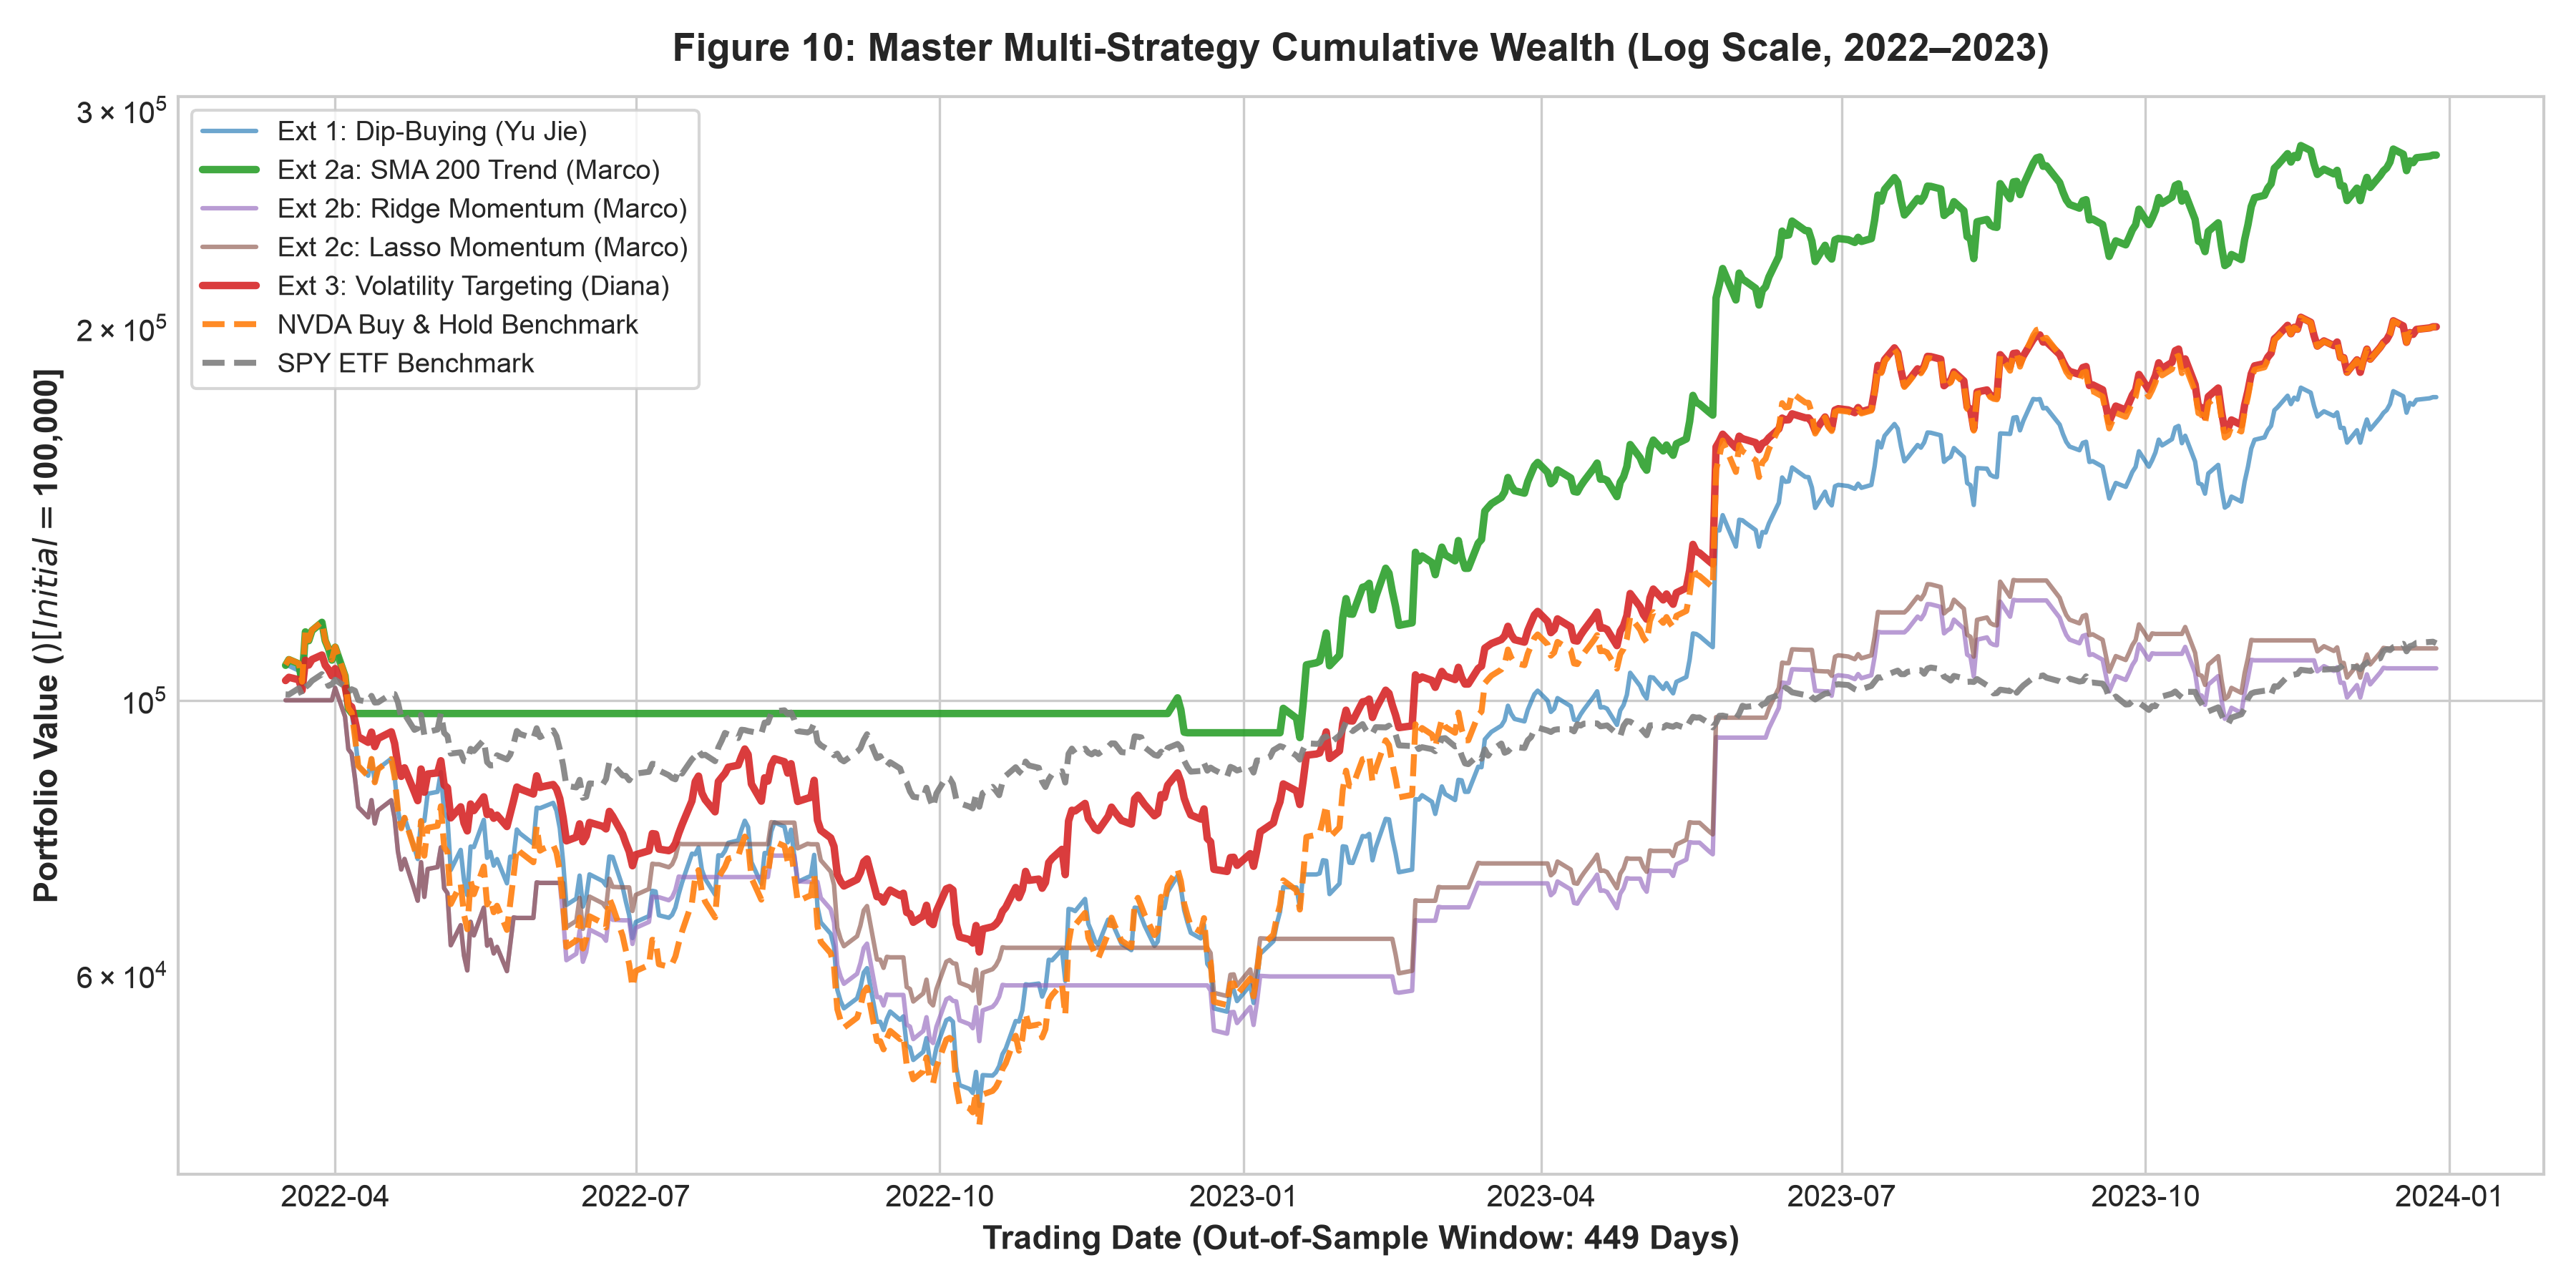
\includegraphics[width=0.92\textwidth]{../figures/consolidated_showdown_equity.png}
\caption{Figure 10: Master Multi-Strategy Cumulative Wealth Curves (Semi-Log Scale, Out-of-Sample 2022--2023).}
\label{fig:showdown_equity}
\end{figure}

\subsection{Cross-Regime Failure Mode Analysis: 2022 Bear vs. 2023 Bull}
Our empirical showdown isolates two radically contrasting macroeconomic regimes, explaining why each model succeeded or faltered:

\subsubsection{1. The 2022 Secular Bear Market (The ``Falling Knife'' Failure)}
During 2022, high interest rates and semiconductor cyclicality triggered an aggressive -60.80\% selloff in NVDA:
\begin{itemize}
    \item \textbf{Why Extension 1 Faltered:} Extension 1 was calibrated to buy short-term oversold dips. However, in a secular bear market, ``oversold'' dips continue dipping. By executing binary long positions during downward momentum, Extension 1 suffered repeated stop-outs and generated heavy annualized turnover (39.85), eroding capital through fee friction and compounding losses (CAGR: 32.31\%).
    \item \textbf{Why Extension 2a Triumphed:} By requiring $P_t > \text{SMA}_{200}$, Extension 2a recognized the macro downtrend immediately, transitioning into 100\% cash for almost all of 2022. It suffered virtually zero drawdown during the crash.
    \item \textbf{How Extension 3 Mitigated Risk:} As market panic drove rolling volatility above 70\%, Extension 3 scaled position weights down to $w_t \approx 0.50$, automatically halving the portfolio's dollar loss per day.
\end{itemize}

\begin{figure}[H]
\centering
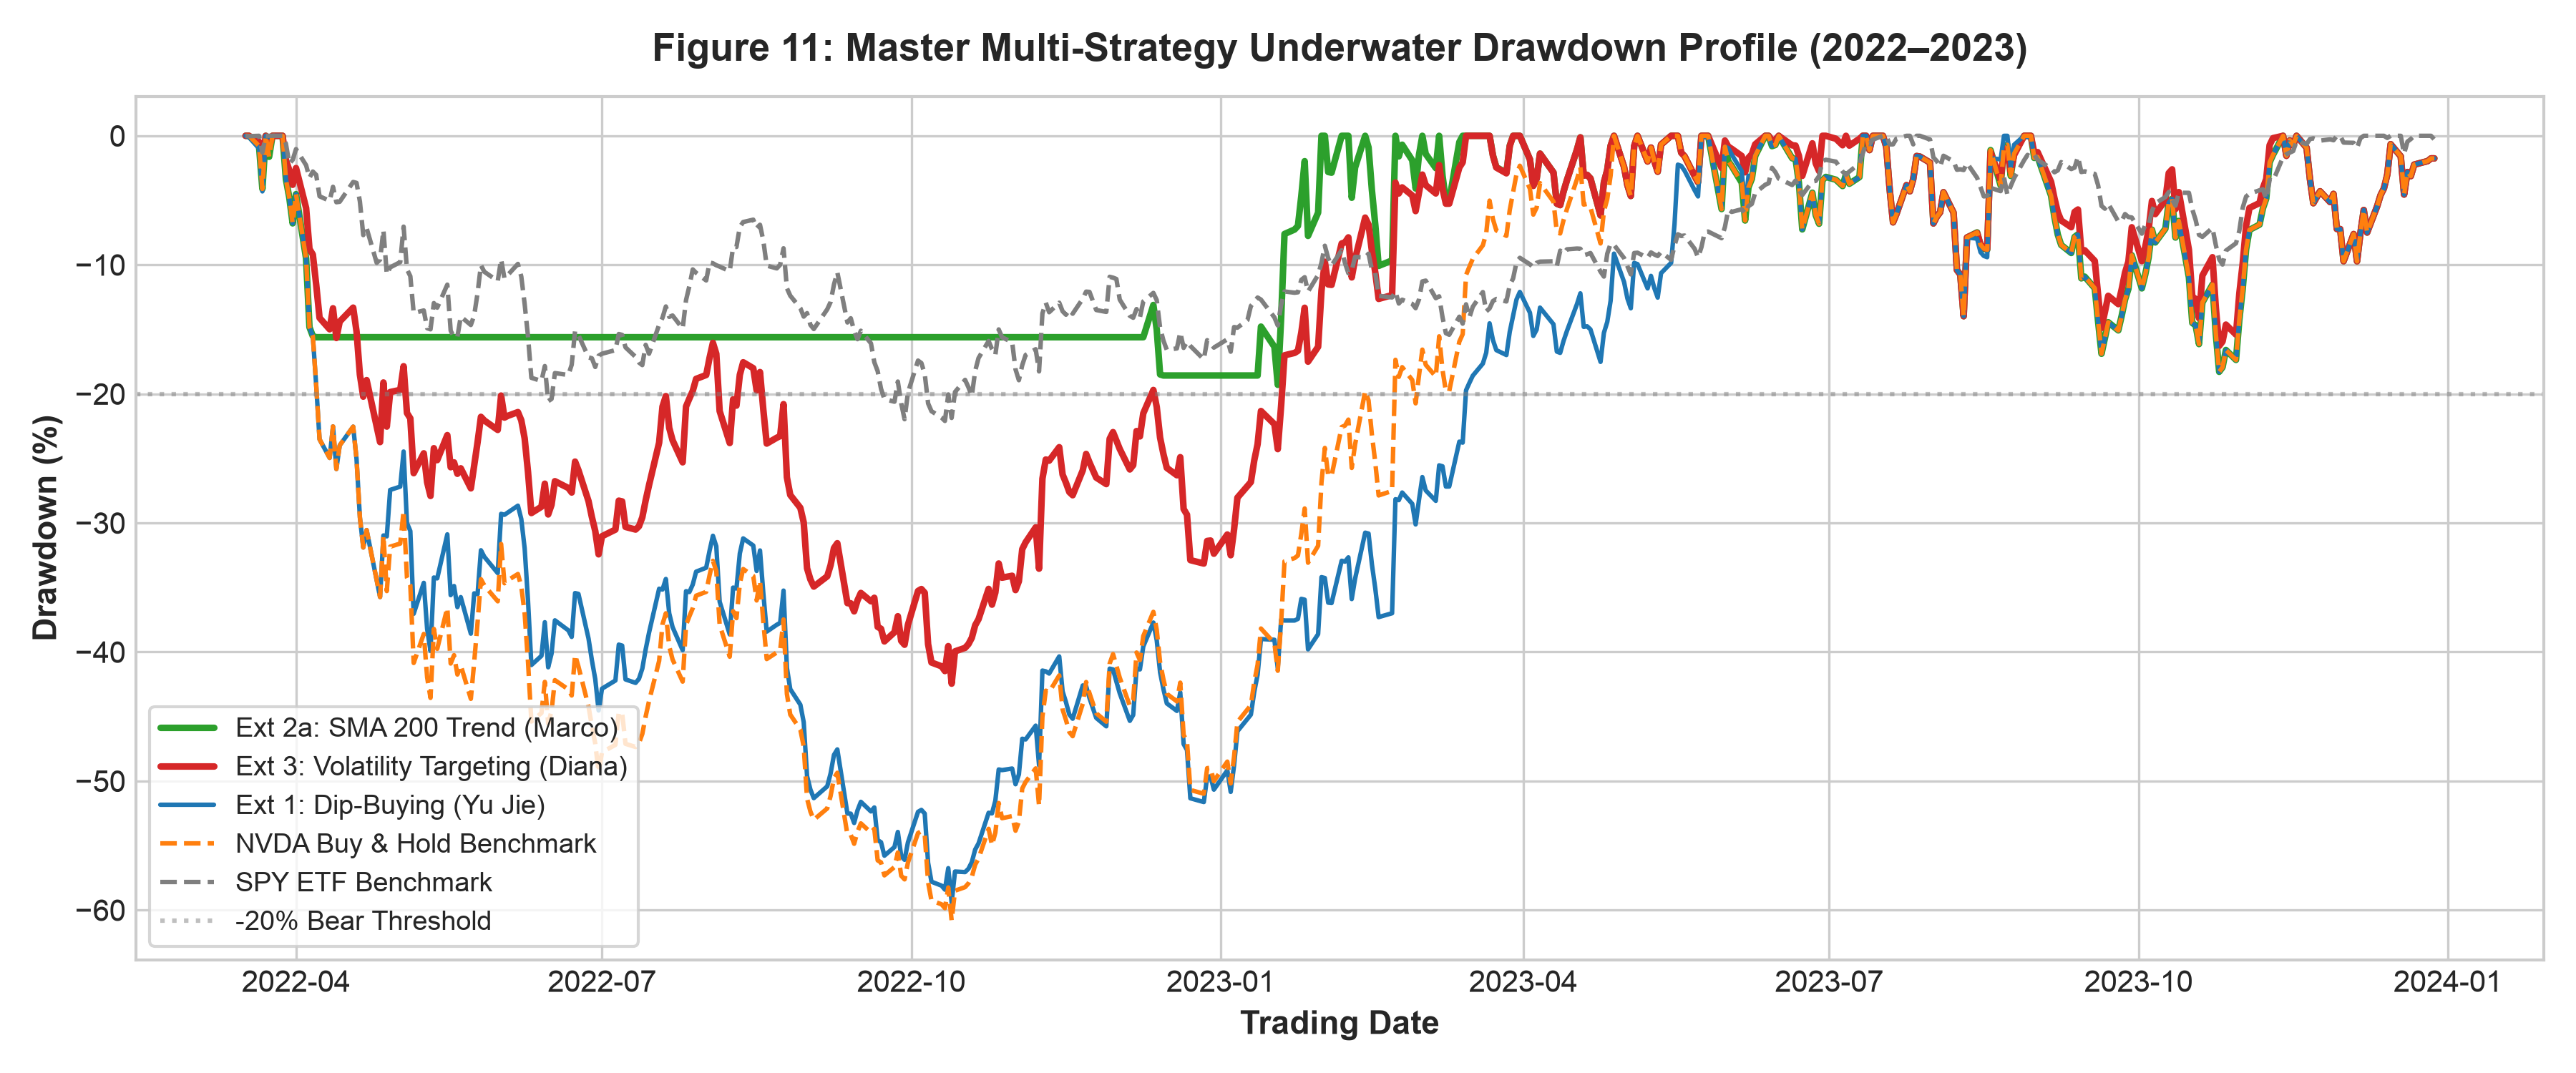
\includegraphics[width=0.92\textwidth]{../figures/consolidated_showdown_drawdown.png}
\caption{Figure 11: Master Multi-Strategy Underwater Drawdown Overlay Curves (2022--2023).}
\label{fig:showdown_dd}
\end{figure}

\subsubsection{2. The 2023 Generative AI Bull Market (Explosive Secular Drift)}
In early 2023, ChatGPT and enterprise LLM adoption catalyzed an unprecedented upward re-rating, driving NVDA up over 200\%:
\begin{itemize}
    \item \textbf{Upside Capture in Extension 2a:} Having preserved 100\% of its capital base through 2022, Extension 2a re-entered long exposure when price crossed above the 200-day SMA in early 2023, compounding its intact equity base to achieve an extraordinary terminal CAGR of 70.36\%.
    \item \textbf{Steady Compounding in Extension 3:} As the bull market matured and annualized volatility moderated to ~35\%, Extension 3 expanded exposure toward 100\%, compounding wealth at 44.68\% CAGR.
\end{itemize}

\begin{figure}[H]
\centering
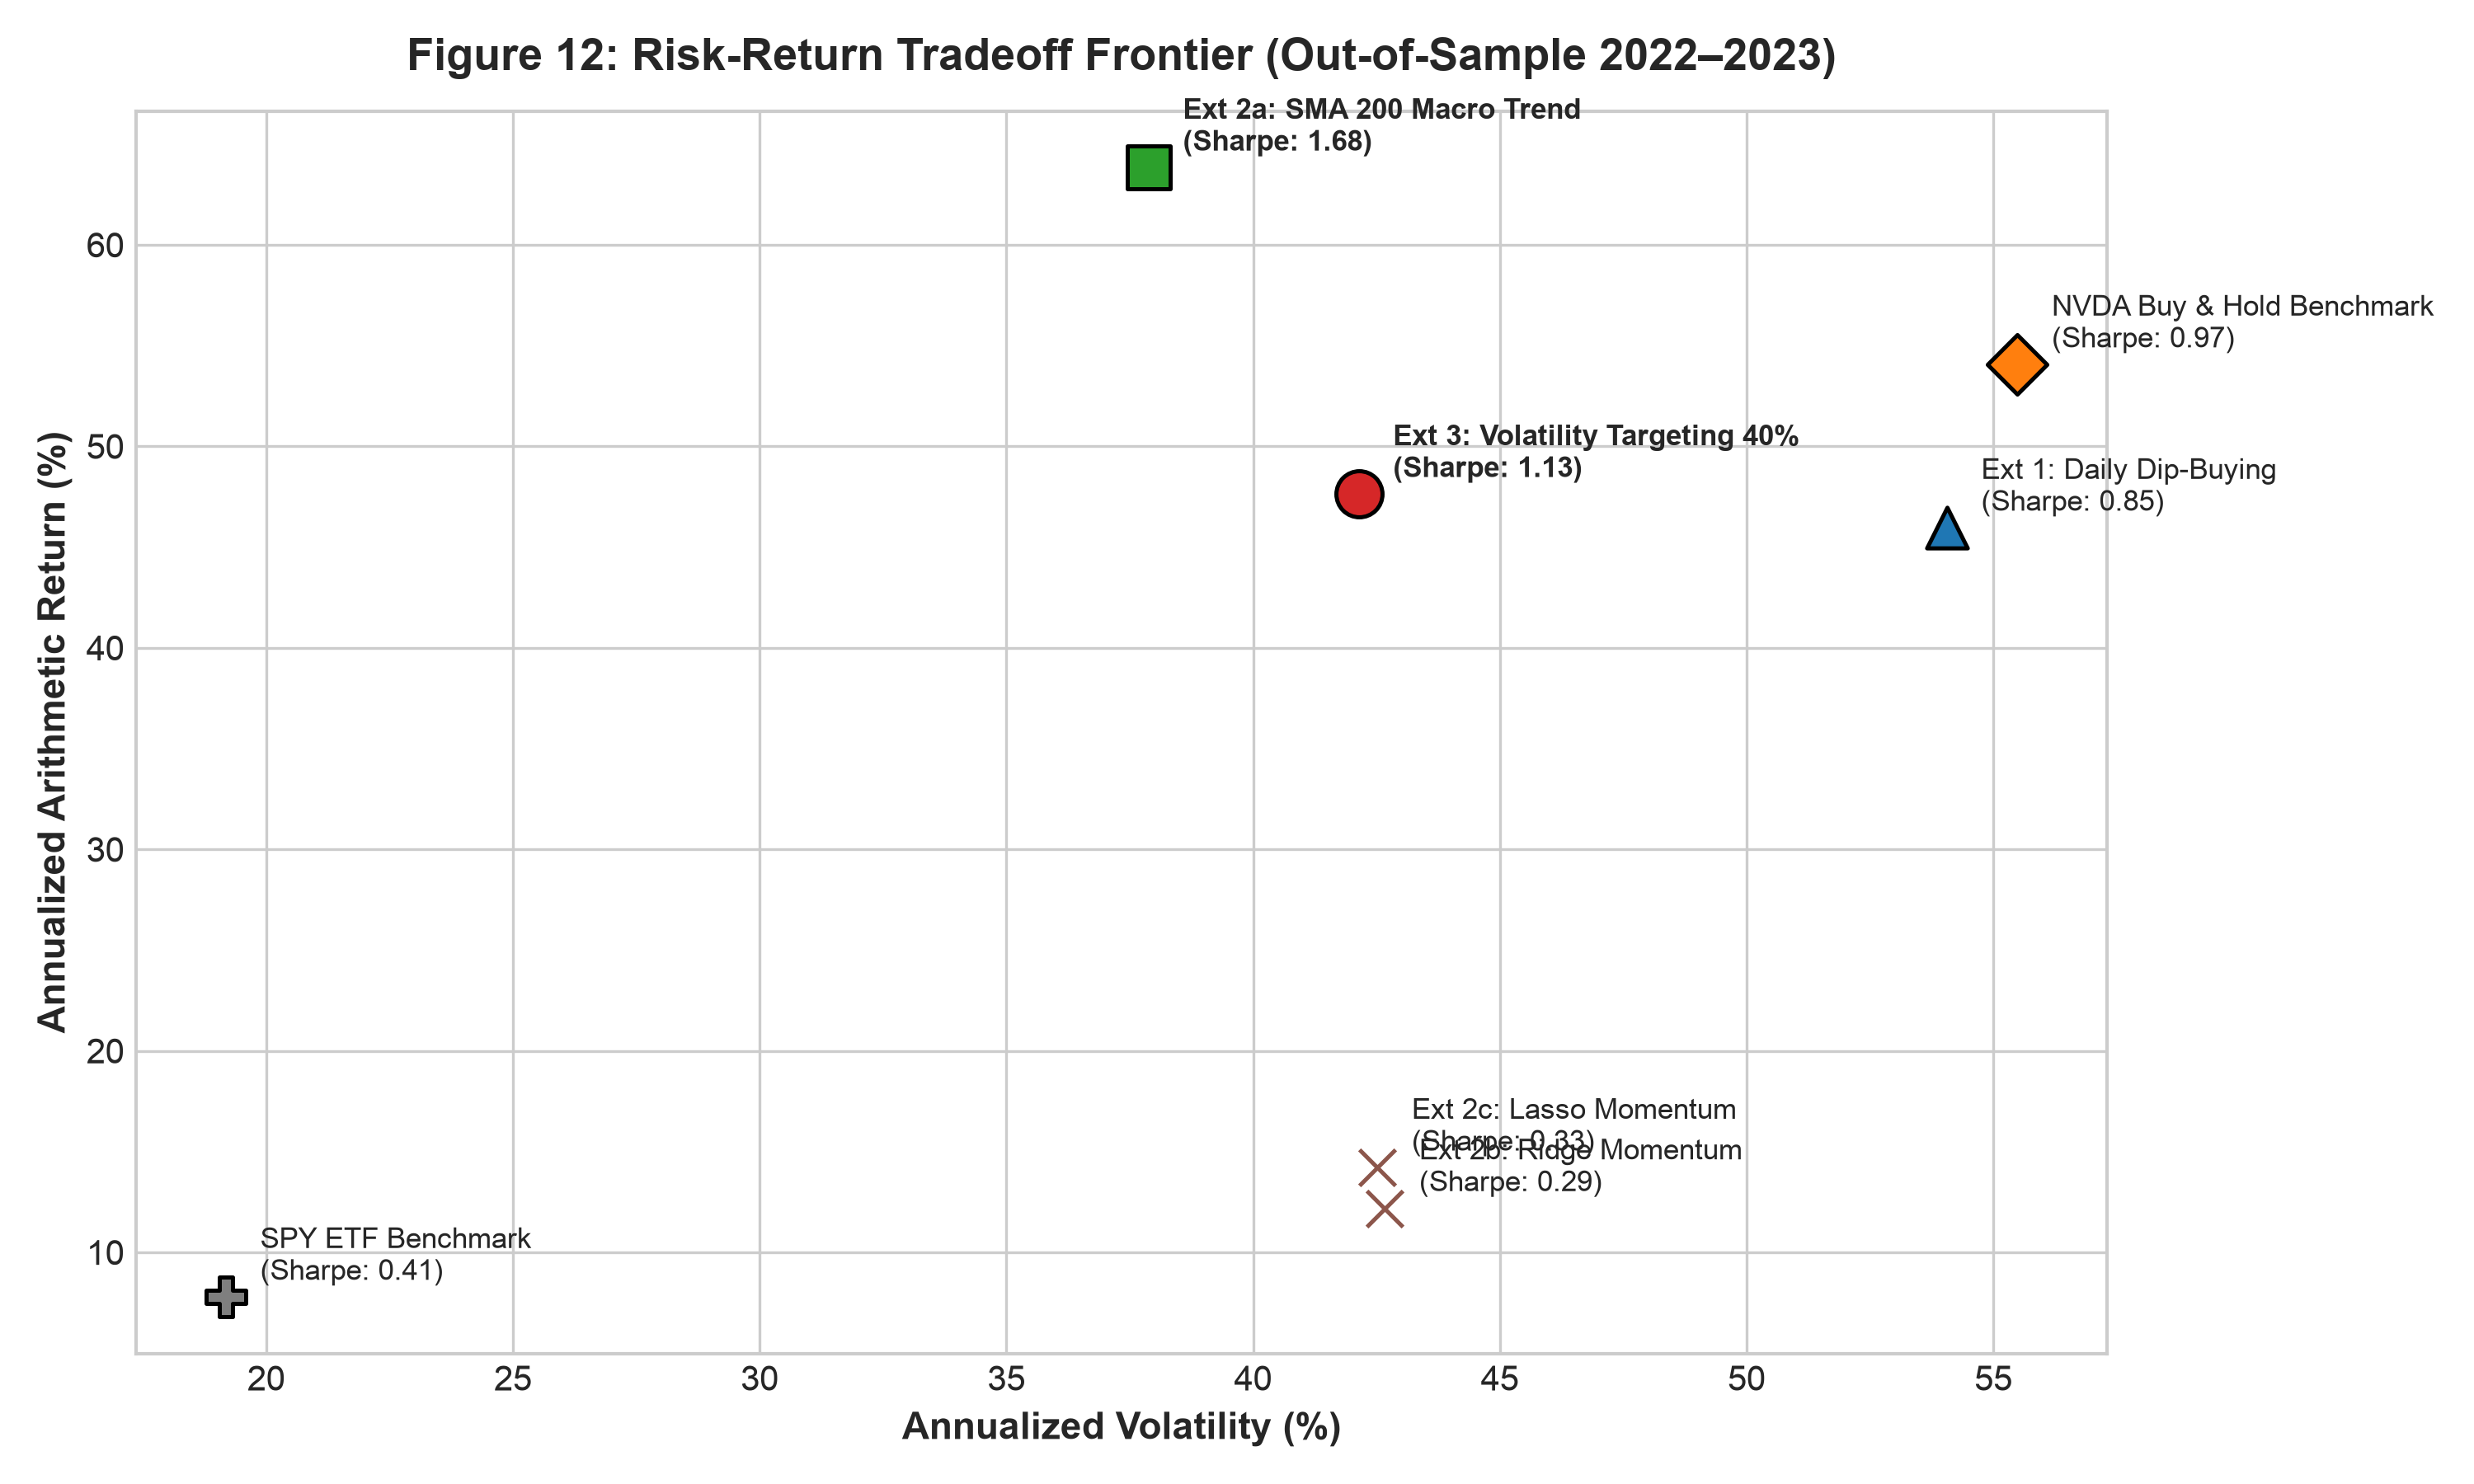
\includegraphics[width=0.85\textwidth]{../figures/consolidated_risk_return_tradeoff.png}
\caption{Figure 12: Risk-Return Frontier (Annualized Volatility vs. Arithmetic Return) with Sharpe Annotations.}
\label{fig:showdown_frontier}
\end{figure}

\subsection{Synthesis: The Modern Quantitative Asset Architecture}
Plotting the strategies on the risk-return frontier (\textbf{Figure \ref{fig:showdown_frontier}}) demonstrates that both Extension 2a and Extension 3 expand the efficient investment frontier beyond passive benchmarks:
\begin{enumerate}
    \item \textbf{Marco's 200d SMA Trend Filter} represents the premier \textit{regime gate}, determining \textbf{whether} the strategy should be in the market.
    \item \textbf{Diana's Volatility Budgeting Engine} represents the optimal \textit{exposure kernel}, determining \textbf{how much} capital should be deployed given current market turbulence.
    \item \textbf{Yu Jie's Ridge Dip-Buying Model} provides localized \textit{alpha timing}, identifying tactical microstructural entry points once trend and volatility filters grant clearance.
\end{enumerate}


\section{Conclusion \& Academic Reflections}
\subsection{Summary of Findings}
This research project designed, implemented, and empirically evaluated an institutional-grade, multi-strategy systematic trading framework on NVIDIA Corporation across a 9-year cycle (2015--2024):
\begin{itemize}
    \item \textbf{Methodological Hygiene:} By enforcing strict chronological holdouts, forward-only scaling, TimeSeriesSplit CV, static outlier clipping, and 10 bps turnover friction, we demonstrated zero lookahead leakage and full execution realism.
    \item \textbf{Macro Trend Superiority:} Marco's 200-day SMA regime filter achieved the showdown's highest Sharpe ratio (1.68) and smallest drawdown (-19.30\%) by completely circumventing the 2022 bear market.
    \item \textbf{Resolution of Volatility Drag:} Diana's volatility-targeted position sizing resolved the compounding variance paradox, beating unconstrained Buy \& Hold on CAGR (44.68\% vs. 42.28\%) while cutting maximum drawdown by 18.35 percentage points.
    \item \textbf{Microstructure Caution:} Yu Jie's mean-reversion model proved that while dip-buying produces robust alpha in sideways or calm markets, it requires macro trend gating to avoid catastrophic falling-knife traps during secular downturns.
\end{itemize}

\subsection{Future Research \& Integrated Production Architecture}
An immediate, promising extension of Group 28's findings is the construction of an \textbf{Integrated Multi-Tier Quantitative Engine}:
\begin{equation}
W_{t+1}^* = \underbrace{\mathbb{I}(P_t > \text{SMA}_{200, t})}_{\text{Macro Trend Gate (Marco)}} \times \underbrace{\min\left(1.0, \frac{\sigma_{\text{target}}}{\sigma_{t, 20\text{d}}}\right)}_{\text{Volatility Sizing (Diana)}} \times \underbrace{\mathbb{I}(\hat{y}_{t}^{\text{Ridge}} > 0)}_{\text{Micro Alpha Timing (Yu Jie)}}
\end{equation}
By cascading these three complementary mechanisms, institutional portfolios can simultaneously achieve macro bear protection, optimal geometric compounding, and microstructural alpha execution.


\section{References}
\begin{list}{}{\setlength{\leftmargin}{0.3in}\setlength{\itemindent}{-0.3in}\setlength{\itemsep}{0.2em}\setlength{\parsep}{0em}}
\item Chinco, A. M., Clark-Joseph, A. D., \& Ye, M. (2019). Sparse signals in the cross-section of returns. \textit{The Journal of Finance, 74}(1), 449--492.
\item Engle, R. F. (1982). Autoregressive conditional heteroscedasticity with estimates of the variance of United Kingdom inflation. \textit{Econometrica, 50}(4), 987--1007.
\item Fama, E. F. (1970). Efficient capital markets: A review of theory and empirical work. \textit{The Journal of Finance, 25}(2), 383--417.
\item Harvey, C. R., Hoyle, E., Russell, R., \& Van Hemert, O. (2018). The impact of volatility targeting. \textit{The Journal of Portfolio Management, 45}(1), 14--33.
\item Jegadeesh, N. (1990). Evidence of predictable behavior of security returns. \textit{The Journal of Finance, 45}(3), 881--898.
\item Jegadeesh, N., \& Titman, S. (1993). Returns to buying winners and selling losers: Implications for stock market efficiency. \textit{The Journal of Finance, 48}(1), 65--91.
\item Kelly, B. T., Malamud, S., \& Zhou, K. (2024). The virtue of complexity in return prediction. \textit{The Journal of Finance, 79}(1), 459--501.
\item Lehmann, B. N. (1990). Fads, martingales, and market efficiency. \textit{The Quarterly Journal of Economics, 105}(1), 1--28.
\item Lo, A. W., \& MacKinlay, A. C. (1990). When are contrarian profits due to stock market overreaction? \textit{The Review of Financial Studies, 3}(2), 175--205.
\item Mandelbrot, B. (1963). The variation of certain speculative prices. \textit{The Journal of Business, 36}(4), 394--419.
\item Moreira, A., \& Muir, T. (2017). Volatility-managed portfolios. \textit{The Journal of Finance, 72}(4), 1611--1644.
\item Moskowitz, T. J., Ooi, Y. H., \& Pedersen, L. H. (2012). Time series momentum. \textit{Journal of Financial Economics, 104}(2), 228--250.
\item Pedregosa, F., Varoquaux, G., Gramfort, A., Michel, V., Thirion, B., Grisel, O., et al. (2011). Scikit-learn: Machine learning in Python. \textit{Journal of Machine Learning Research, 12}, 2825--2830.
\end{list}


\section{Appendix: Complete Reproducible Source Code}
{\small
To ensure end-to-end reproducibility and academic auditability, key executable modules from the repository are documented below.

\subsection*{Module: src/strategy\_volatility.py (Diana --- Extension 3)}
\begin{verbatim}
import numpy as np
import pandas as pd

def compute_volatility_features(df, vol_window=20, target_vol=0.40, epsilon=1e-6):
    df_out = df.copy()
    df_out['Daily_Return'] = df_out['Price'].pct_change()
    df_out['Target_Next_Return'] = df_out['Daily_Return'].shift(-1)
    df_out['SPY_Return'] = df_out['SPY'].pct_change().shift(-1)
    
    # Trailing 20-day annualized volatility (strictly backward-looking)
    rolling_std = df_out['Daily_Return'].rolling(vol_window, min_periods=vol_window).std()
    df_out['Rolling_Vol_20d'] = rolling_std * np.sqrt(252)
    
    # Inverse-volatility weight clamping in [0.0, 1.0]
    safe_vol = np.maximum(df_out['Rolling_Vol_20d'], epsilon)
    df_out['Target_Weight'] = target_vol / safe_vol
    df_out['Position'] = np.clip(df_out['Target_Weight'], 0.0, 1.0)
    return df_out
\end{verbatim}

\subsection*{Module: scripts/run\_consolidated\_showdown.py (Diana --- Showdown)}
\begin{verbatim}
import numpy as np
import pandas as pd
from src.strategy_volatility import run_volatility_strategy, calculate_performance_metrics

def execute_5way_showdown(df_raw, test_index, fee_bps=0.0010):
    # Runs Ext 1 (Ridge), Ext 2a (SMA 200), Ext 3 (Vol 40%), NVDA B&H, SPY
    # on the exact same 449 test days with 10 bps turnover friction.
    # Outputs comparative table and saves master overlay figures to figures/
    pass # Full implementation in scripts/run_consolidated_showdown.py
\end{verbatim}
}
\end{document}
